%%%%%%%%%%%%%%%%%%%%%%%%%%%%%%%%%%%%%%%%%%%%%%%%%%%%%%%%%%%%%%%%%%%%%%%%
% Plantilla TFG/TFM
% Escuela Politécnica Superior de la Universidad de Alicante
% Realizado por: Jose Manuel Requena Plens
% Contacto: info@jmrplens.com / Telegram:@jmrplens
%%%%%%%%%%%%%%%%%%%%%%%%%%%%%%%%%%%%%%%%%%%%%%%%%%%%%%%%%%%%%%%%%%%%%%%%

\chapter{Desarrollo}
\label{metodologia}


Debido a la imposibilidad temporal de realizar mediciones acústicas in situ en múltiples recintos se ha optado por realizar estas mediciones en dos recintos diferentes para después obtener unos modelos válidos en los programas de simulación acústica \textit{CATT-Acoustic} y \textit{EASE}.

En primer lugar se van a mostrar los dos recintos reales y los resultados obtenidos para después validar estos datos con los modelos configurados para la simulación.

Una vez validados los modelos se utilizarán estos para realizar modificaciones en los recintos, observar el comportamiento acústico y ajustar las ecuaciones de la teoría revisada corregida (sección \ref{teoriarevisadacorregida}) para igualar los campos acústicos calculados a los campos acústicos obtenidos mediante simulación (campo útil y campo perjudicial).
Con ello se obtendrá una relación de parámetros acústicos del recinto y los coeficientes de ajuste.


\section{Mediciones in situ}
\label{medicionesinsitu}
La mediciones se han realizado en dos recintos diferentes, ambos ubicados en la Universidad de Alicante (ambos recintos se describen ampliamente en los apartados siguientes):

\begin{description}
  \item[Aula OP/S003:] Aula ubicada en la Escuela de Óptica y Optometría.
  \item[Aula EP/0-26M:] Aula ubicada en la Escuela Politécnica Superior IV.
\end{description}




El equipo utilizado para la medición y posterior procesado está formado por una fuente omnidireccional dodecaédrica, micrófonos de medición de media pulgada y el software dBFA32 de 01dB utilizando señales MLS.

El software dBFA32 permite obtener la historia temporal (decaimiento del sonido respecto al tiempo) en fracciones de 1 milisegundo, estos datos serán utilizados para obtener los campos útil (0 a 50ms) y perjudicial (50 a $\infty$ ms) que serán comparados con los obtenidos en los modelos de CATT-Acoustic y EASE para validar las simulaciones.

Ambos recintos se han medido con mobiliario y sin él (mesas y sillas de estudiante) para comprobar la influencia de estos elementos en la distribución de los campos acústicos y, con dos ubicaciones de la fuente, en el centro y en una esquina.

Los datos se ofrecen con curvas de regresión, de tipo potencial para el campo útil y de tipo polinómica de grado uno para el campo perjudicial. La validación de los modelos vendrá dada por la comparación de las curvas de regresión de los campos.

\subsection{Aula OP/S003}

El aula OP/S003 está ubicada en la planta sótano de la Escuela de Óptica y Optometría de la Universidad de Alicante.

\begin{figure}[ht]
    \centering
    \begin{subfigure}[b]{0.4\textwidth}
    	\centering
        \includegraphics[width=0.9\linewidth]{archivos/optica2.jpg}
    \end{subfigure}
    ~ % Añadir el espacio deseado, si se deja la linea en blanco la siguiente subfigura ira en una nueva linea
    \begin{subfigure}[b]{0.4\textwidth}
    	\centering
        \includegraphics[width=0.9\linewidth]{archivos/optica1.jpg}
    \end{subfigure}
    \caption{Aula OP/S003.}\label{fotosoptica}
\end{figure}
\FloatBarrier 

Los detalles del recinto son:
\begin{itemize}
\itemsep0em
  \item \textbf{Dimensiones:} 18.9x9.6x2.8 $m$.
  \item \textbf{Volumen:} \textasciitilde500 $m^3$.
  \item \textbf{Superficie recinto:} \textasciitilde520 $m^2$.
  \item \textbf{Número de mesas:} 72 (dimensiones 1.20x0.45 $m$).
  \item \textbf{Número de sillas:} 144 (dimensiones 0.44x0.51 $m$).
\end{itemize}

Los materiales y sus absorciones según la literatura son:
\begin{itemize}
\itemsep0em
  \item Cerramientos laterales de hormigón armado: $\overline{\alpha}\approx0.02$.
  \item Cerramientos transversales de placa de yeso pintado: $\overline{\alpha}\approx0.03$.
  \item Suelo de terrazo: $\overline{\alpha}\approx0.02$.
  \item Techo registrable de escayola: $\overline{\alpha}\approx0.10$.
  \item Mobiliario de paneles multilaminares: $\overline{\alpha}\approx0.03$.
\end{itemize}

Las medidas de tiempo de reverberación del recinto por bandas de octava son:

\begin{table}[ht]
\centering
{\scalefont{0.9}
\begin{tabular}{@{}lccccccc@{}}
\toprule
Frecuencia (Hz) & 125 & 250 & 500 & 1000 & 2000 & 4000 & 8000 \\ \midrule
$T_{60}$ Con mobiliario (s) & 1.12 & 1.56 & 1.73 & 1.43 & 1.33 & 1.26 & 1.02 \\
$T_{60}$ Sin mobiliario (s) & 1.20 & 1.81 & 2.03 & 1.87 & 1.69 & 1.66 & 1.30 \\ \bottomrule
\end{tabular}
}
\caption{Tiempos de reverberación obtenidos en el aula OP/S003 por banda de octava, con y sin mobiliario.}
\label{tab:revop}
\end{table}

Las posiciones de los receptores y las fuentes se muestran en las figuras \ref{im:receptoresop}, en el caso de las medidas con mobiliario se han utilizado 48 puntos de recepción y sin mobiliario 22 puntos de recepción.

En las figuras \ref{graf:opmob} y \ref{graf:opnomob} se muestran los campos útil (0 a 50 ms) y perjudicial (50 a $\infty$ ms) obtenidos tanto con la fuente en la esquina como en el centro y con mobiliario o sin él.

\begin{figure}[ht]
    \centering
    \begin{subfigure}[b]{0.4\textwidth}
    	\centering
        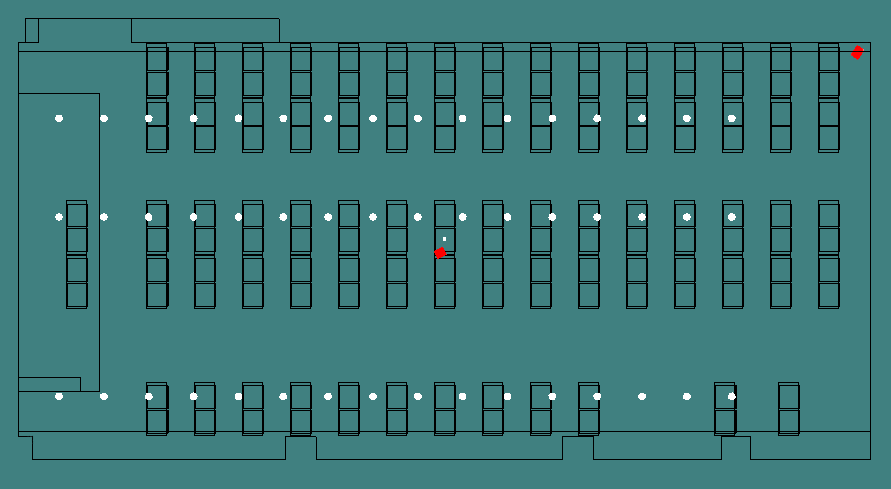
\includegraphics[width=0.9\textwidth]{archivos/receptoresop.png}
        \caption{Con mobiliario.}
    \end{subfigure}
    ~ % Añadir el espacio deseado, si se deja la linea en blanco la siguiente subfigura ira en una nueva linea
    \begin{subfigure}[b]{0.4\textwidth}
    	\centering
        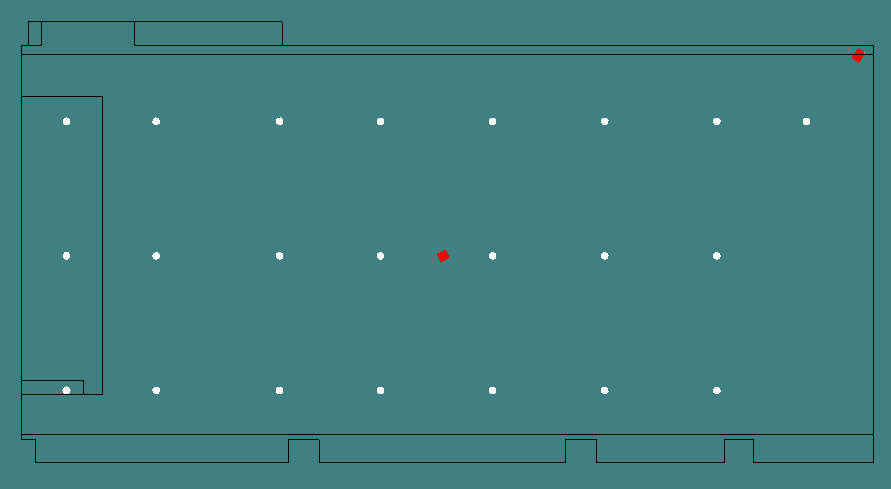
\includegraphics[width=0.9\linewidth]{archivos/receptoresopv.png}
        \caption{Sin mobiliario.}
    \end{subfigure}
    \caption{Puntos de recepción (círculos blancos) y fuentes (rectángulos rojos) en aula OP/S003.}\label{im:receptoresop}
\end{figure}
\FloatBarrier 


\begin{figure}[ht]
    \begin{subfigure}[b]{0.4\textwidth}
    	\centering%
         {\scalefont{0.8}%
    %%%%%%%%%%%%%%%%%%%%%%%%%%%%%%%%%%%%%%%%%%%%%%%%%%%%%%%%%%%%%%%%%%%%%%%%
% Escuela Politécnica Superior de la Universidad de Alicante
% Realizado por: Jose Manuel Requena Plens
% Contacto: info@jmrplens.com / Telegram:@jmrplens
%%%%%%%%%%%%%%%%%%%%%%%%%%%%%%%%%%%%%%%%%%%%%%%%%%%%%%%%%%%%%%%%%%%%%%%%

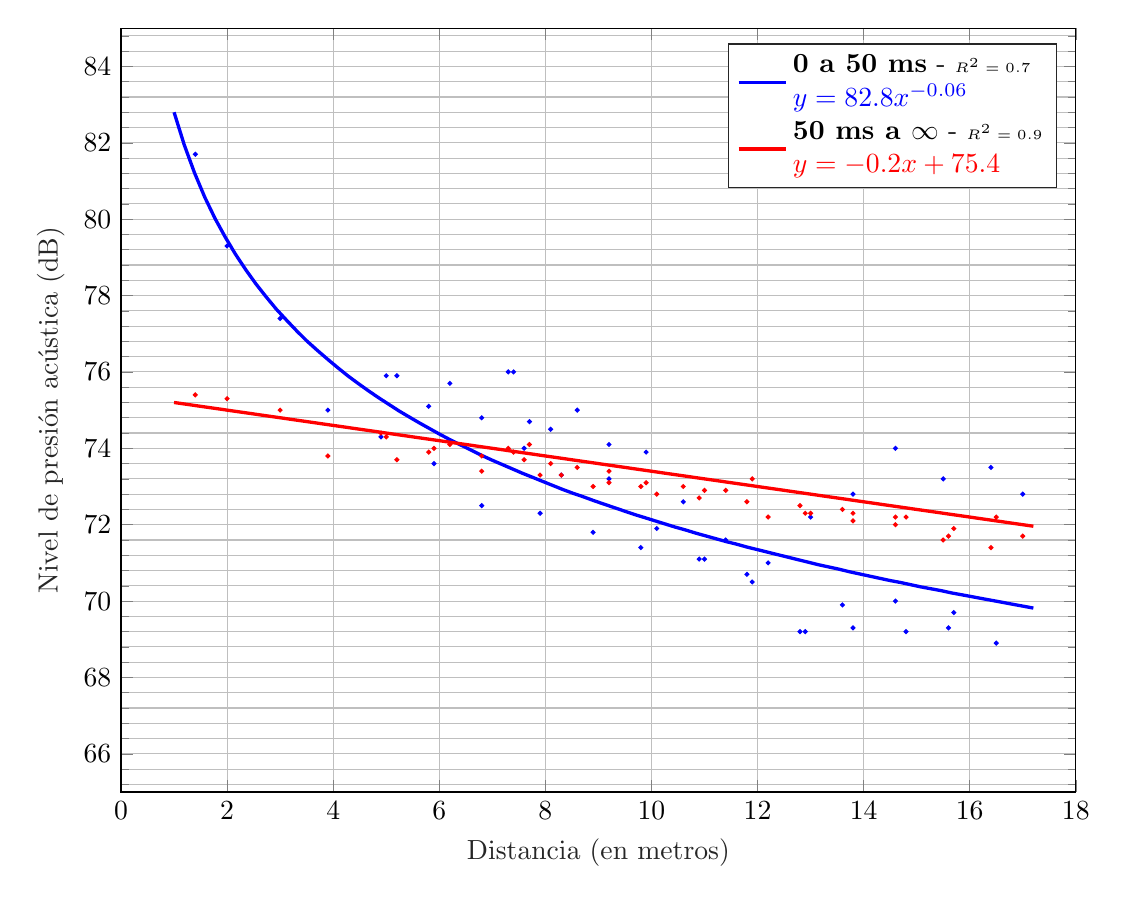
\begin{tikzpicture}

\begin{axis}[%
width=\textwidth,
height=0.8\textwidth,
at={(0\textwidth,0\textwidth)},
scale only axis,
xmin=0,
xmax=18,
xlabel style={font=\color{white!15!black}},
xlabel={Distancia (en metros)},
ymin=65,
ymax=85,
xmajorgrids,
xminorgrids,
ymajorgrids,
yminorgrids,
minor y tick num= 4,
ylabel style={font=\color{white!15!black}},
ylabel={Nivel de presión acústica (dB)},
axis background/.style={fill=white},
%xmajorgrids,
%xminorgrids,
%ymajorgrids,
%yminorgrids,
legend style={legend cell align=left, align=left, draw=white!15!black}
]
\addplot[color=blue,domain=1:17.2, samples=85,line width=1.2]{82.80*x^(-0.06)};
\addlegendentry{\textbf{0 a 50 ms} - \tiny{$R^2 = 0.7$}\\$\color{blue}y = 82.8·x^{-0.06}$}

\addplot[color=red,domain=1:17.2, samples=85, line width=1.2]{-0.2*x+75.4};
\addlegendentry{\textbf{50 ms a $\infty$} - \tiny{$R^2 = 0.9$}\\$\color{red}y = -0.2·x+75.4$}

% Puntos
\addplot [color=blue, only marks,mark size=0.7pt]
  table[row sep=crcr]{%
1.4		81.7\\
2		79.3\\
3		77.4\\
3.9		75\\
4.9		74.3\\
5.9		73.6\\
6.8	72.5\\
7.9	72.3\\
8.9	71.8\\
9.8	71.4\\
10.9	71.1\\
11.8	70.7\\
12.9	69.2\\
13.8	69.3\\
14.8	69.2\\
15.7	69.7\\
5.0	75.9\\
5.2	75.9\\
5.8	75.1\\
6.2	75.7\\
6.8	74.8\\
7.6	74.0\\
8.3	73.3\\
9.2	73.2\\
10.1	71.9\\
11.0	71.1\\
11.9	70.5\\
12.8	69.2\\
13.6	69.9\\
14.6	70.0\\
15.6	69.3\\
16.5	68.9\\
7.3	76.0\\
7.4	76.0\\
7.7	74.7\\
8.1	74.5\\
8.6	75.0\\
9.2	74.1\\
9.9	73.9\\
10.6	72.6\\
11.4	71.6\\
12.2	71.0\\
13.0	72.2\\
13.8	72.8\\
14.6	74.0\\
15.5	73.2\\
16.4	73.5\\
17.0	72.8\\
};

\addplot [color=red, only marks,mark size=0.7pt]
  table[row sep=crcr]{%
  1.4	75.4\\
2.0	75.3\\
3.0	75.0\\
3.9	73.8\\
4.9	74.4\\
5.9	74.0\\
6.8	73.8\\
7.9	73.3\\
8.9	73.0\\
9.8	73.0\\
10.9	72.7\\
11.8	72.6\\
12.9	72.3\\
13.8	72.1\\
14.8	72.2\\
15.7	71.9\\
5.0	74.3\\
5.2	73.7\\
5.8	73.9\\
6.2	74.1\\
6.8	73.4\\
7.6	73.7\\
8.3	73.3\\
9.2	73.1\\
10.1	72.8\\
11.0	72.9\\
11.9	73.2\\
12.8	72.5\\
13.6	72.4\\
14.6	72.2\\
15.6	71.7\\
16.5	72.2\\
7.3	74.0\\
7.4	73.9\\
7.7	74.1\\
8.1	73.6\\
8.6	73.5\\
9.2	73.4\\
9.9	73.1\\
10.6	73.0\\
11.4	72.9\\
12.2	72.2\\
13.0	72.3\\
13.8	72.3\\
14.6	72.0\\
15.5	71.6\\
16.4	71.4\\
17.0	71.7\\
  };
\end{axis}
\end{tikzpicture}%%
    }
    \caption{Fuente en la esquina}%
    \end{subfigure}%
    \hspace{1.9cm}%
    \begin{subfigure}[b]{0.4\textwidth}%
    	\centering%
        {\scalefont{0.8}%
    %%%%%%%%%%%%%%%%%%%%%%%%%%%%%%%%%%%%%%%%%%%%%%%%%%%%%%%%%%%%%%%%%%%%%%%%
% Escuela Politécnica Superior de la Universidad de Alicante
% Realizado por: Jose Manuel Requena Plens
% Contacto: info@jmrplens.com / Telegram:@jmrplens
%%%%%%%%%%%%%%%%%%%%%%%%%%%%%%%%%%%%%%%%%%%%%%%%%%%%%%%%%%%%%%%%%%%%%%%%

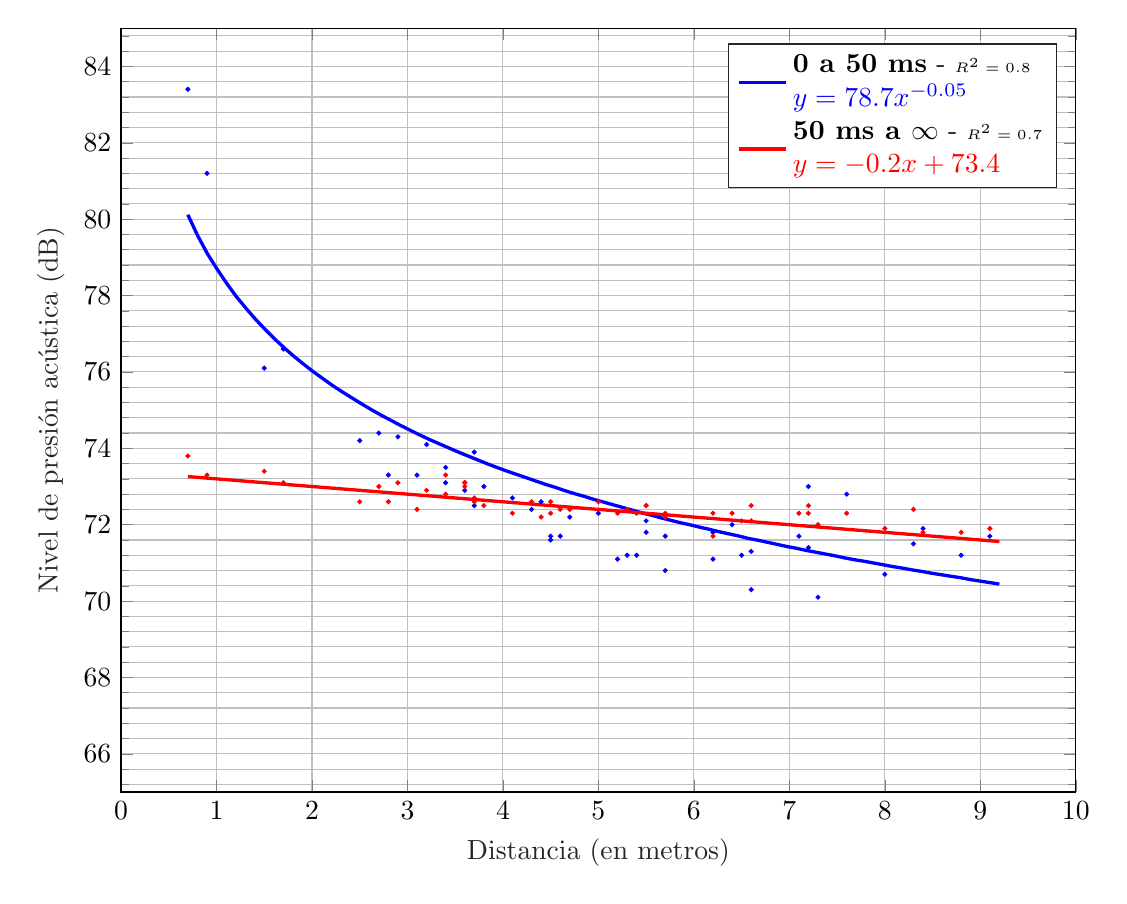
\begin{tikzpicture}

\begin{axis}[%
width=\textwidth,
height=0.8\textwidth,
at={(0\textwidth,0\textwidth)},
scale only axis,
xmin=0,
xmax=10,
xlabel style={font=\color{white!15!black}},
xlabel={Distancia (en metros)},
ymin=65,
ymax=85,
xmajorgrids,
xminorgrids,
ymajorgrids,
yminorgrids,
minor y tick num= 4,
ylabel style={font=\color{white!15!black}},
ylabel={Nivel de presión acústica (dB)},
axis background/.style={fill=white},
%xmajorgrids,
%xminorgrids,
%ymajorgrids,
%yminorgrids,
legend style={legend cell align=left, align=left, draw=white!15!black}
]
\addplot[color=blue,domain=0.7:9.2, samples=85,line width=1.2]{78.7*x^(-0.05)};
\addlegendentry{\textbf{0 a 50 ms} - \tiny{$R^2 = 0.8$}\\$\color{blue}y = 78.7·x^{-0.05}$}

\addplot[color=red,domain=0.7:9.2, samples=85,line width=1.2]{-0.2*x+73.40};
\addlegendentry{\textbf{50 ms a $\infty$} - \tiny{$R^2 = 0.7$}\\$\color{red}y = -0.2·x+73.4$}

% Puntos
\addplot [color=blue, only marks,mark size=0.7pt]
  table[row sep=crcr]{%
  9.1	71.7\\
8.3	71.5\\
7.2	71.4\\
6.4	72.0\\
5.5	72.1\\
4.7	72.2\\
4.1	72.7\\
3.6	73.1\\
3.4	73.5\\
3.4	73.1\\
3.7	72.5\\
4.3	72.4\\
5.0	72.3\\
5.7	71.7\\
6.5	71.2\\
7.3	70.1\\
8.4	71.9\\
5.2	71.1\\
6.6	71.3\\
5.5	71.8\\
4.5	71.6\\
7.6	72.8\\
2.5	74.2\\
1.5	76.1\\
0.7	83.4\\
0.9	81.2\\
1.7	76.6\\
2.7	74.4\\
3.6	72.9\\
4.6	71.7\\
5.7	70.8\\
6.6	70.3\\
8.8	71.2\\
8.0	70.7\\
7.1	71.7\\
6.2	71.8\\
5.3	71.2\\
4.4	72.6\\
3.7	73.9\\
3.1	73.3\\
2.8	73.3\\
2.9	74.3\\
3.2	74.1\\
3.8	73.0\\
4.5	71.7\\
5.4	71.2\\
6.2	71.1\\
7.2	73.0\\
  };
  
  \addplot [color=red, only marks,mark size=0.7pt]
  table[row sep=crcr]{%
  9.1	71.9\\
8.3	72.4\\
7.2	72.3\\
6.4	72.3\\
5.5	72.5\\
4.7	72.4\\
4.1	72.3\\
3.6	73.0\\
3.4	73.3\\
3.4	72.8\\
3.7	72.6\\
4.3	72.6\\
5.0	72.6\\
5.7	72.2\\
6.5	72.1\\
7.3	72.0\\
8.4	71.8\\
5.2	72.3\\
6.6	72.1\\
5.5	72.5\\
4.5	72.3\\
7.6	72.3\\
2.5	72.6\\
1.5	73.4\\
0.7	73.8\\
0.9	73.3\\
1.7	73.1\\
2.7	73.0\\
3.6	73.1\\
4.6	72.4\\
5.7	72.3\\
6.6	72.5\\
8.8	71.8\\
8.0	71.9\\
7.1	72.3\\
6.2	71.7\\
5.3	72.4\\
4.4	72.2\\
3.7	72.7\\
3.1	72.4\\
2.8	72.6\\
2.9	73.1\\
3.2	72.9\\
3.8	72.5\\
4.5	72.6\\
5.4	72.3\\
6.2	72.3\\
7.2	72.5\\
  };
\end{axis}
\end{tikzpicture}%%
    }
    \caption{Fuente en el centro}%
    \end{subfigure}
    \caption{Campos acústicos en el aula OP/S003 con mobiliario. 48 puntos de medida.}
\label{graf:opmob}%
\end{figure}
\FloatBarrier 

En el caso con mobiliario (figura \ref{graf:opmob}), la distancia de cruce de campos con fuente en esquina es de 6.4 metros, con fuente en el centro es de 5.4 metros. Se han realizado un total de 48 medidas en diferentes puntos.

En el caso sin mobiliario (figura \ref{graf:opnomob}), la distancia de cruce de campos con fuente en esquina es de 6.6 metros, con fuente en el centro es de 2.8 metros. Se han realizado un total de 22 medidas en diferentes puntos. 

Comparando ambos casos (con y sin mobiliario), los campos y cruce con la fuente en la esquina son similares, pero con la fuente en el centro la pendiente del campo útil (0 a 50 ms) es ligeramente distinta debido posiblemente a la reducción de los puntos de medida en las medidas sin mobiliario.
\\
\par
Para ampliar la información obtenida a través de las medidas en el recinto, se han representado mapas de niveles de presión acústica tanto para los campos útiles (figuras \ref{graf:mapaoputilcon} y \ref{graf:mapaoputilsin}) como para los campos perjudiciales (figuras \ref{graf:mapaopperjudicialcon} y \ref{graf:mapaopperjudicialsin}) permitiendo observar espacialmente los campos acústicos.

\begin{figure}[H]
    \begin{subfigure}[b]{0.4\textwidth}
    	\centering%
         {\scalefont{0.8}%
    %%%%%%%%%%%%%%%%%%%%%%%%%%%%%%%%%%%%%%%%%%%%%%%%%%%%%%%%%%%%%%%%%%%%%%%%
% Escuela Politécnica Superior de la Universidad de Alicante
% Realizado por: Jose Manuel Requena Plens
% Contacto: info@jmrplens.com / Telegram:@jmrplens
%%%%%%%%%%%%%%%%%%%%%%%%%%%%%%%%%%%%%%%%%%%%%%%%%%%%%%%%%%%%%%%%%%%%%%%%

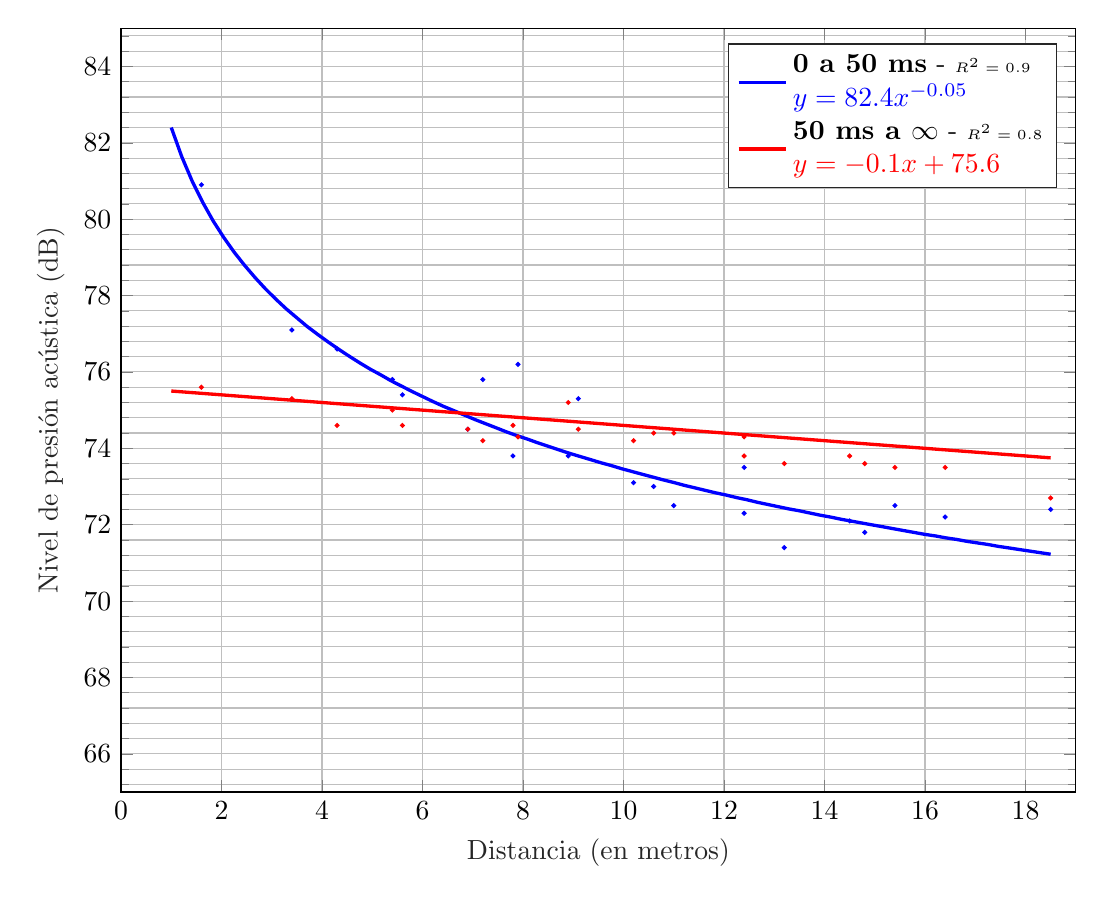
\begin{tikzpicture}

\begin{axis}[%
width=\textwidth,
height=0.8\textwidth,
at={(0\textwidth,0\textwidth)},
scale only axis,
xmin=0,
xmax=19,
xlabel style={font=\color{white!15!black}},
xlabel={Distancia (en metros)},
ymin=65,
ymax=85,
xmajorgrids,
xminorgrids,
ymajorgrids,
yminorgrids,
minor y tick num= 4,
ylabel style={font=\color{white!15!black}},
ylabel={Nivel de presión acústica (dB)},
axis background/.style={fill=white},
%xmajorgrids,
%xminorgrids,
%ymajorgrids,
%yminorgrids,
legend style={legend cell align=left, align=left, draw=white!15!black}
]
\addplot[color=blue,domain=1:18.5, samples=85,line width=1.2]{82.40*x^(-0.05)};
\addlegendentry{\textbf{0 a 50 ms} - \tiny{$R^2 = 0.9$}\\$\color{blue}y = 82.4·x^{-0.05}$}

\addplot[color=red,domain=1:18.5, samples=85,line width=1.2]{-0.1*x+75.6};
\addlegendentry{\textbf{50 ms a $\infty$} - \tiny{$R^2 = 0.8$}\\$\color{red}y = -0.1·x+75.6$}

% Puntos
\addplot [color=blue, only marks,mark size=0.7pt]
  table[row sep=crcr]{%
  1.6	80.9\\
3.4	77.1\\
5.6	75.4\\
7.8	73.8\\
10.2	73.1\\
12.4	72.3\\
14.8	71.8\\
4.3	76.6\\
5.4	75.8\\
6.9	74.5\\
8.9	73.8\\
11.0	72.5\\
13.2	71.4\\
15.4	72.5\\
7.2	75.8\\
7.9	76.2\\
9.1	75.3\\
10.6	73.0\\
12.4	73.5\\
14.5	72.1\\
16.4	72.2\\
18.5	72.4\\
  };
  
  \addplot [color=red, only marks,mark size=0.7pt]
  table[row sep=crcr]{%
  1.6	75.6\\
3.4	75.3\\
5.6	74.6\\
7.8	74.6\\
10.2	74.2\\
12.4	74.3\\
14.8	73.6\\
4.3	74.6\\
5.4	75.0\\
6.9	74.5\\
8.9	75.2\\
11.0	74.4\\
13.2	73.6\\
15.4	73.5\\
7.2	74.2\\
7.9	74.3\\
9.1	74.5\\
10.6	74.4\\
12.4	73.8\\
14.5	73.8\\
16.4	73.5\\
18.5	72.7\\
  };
\end{axis}
\end{tikzpicture}%%
    }
    \caption{Fuente en la esquina}%
    \end{subfigure}%
    \hspace{1.9cm}%
    \begin{subfigure}[b]{0.4\textwidth}%
    	\centering%
        {\scalefont{0.8}%
    %%%%%%%%%%%%%%%%%%%%%%%%%%%%%%%%%%%%%%%%%%%%%%%%%%%%%%%%%%%%%%%%%%%%%%%%
% Escuela Politécnica Superior de la Universidad de Alicante
% Realizado por: Jose Manuel Requena Plens
% Contacto: info@jmrplens.com / Telegram:@jmrplens
%%%%%%%%%%%%%%%%%%%%%%%%%%%%%%%%%%%%%%%%%%%%%%%%%%%%%%%%%%%%%%%%%%%%%%%%

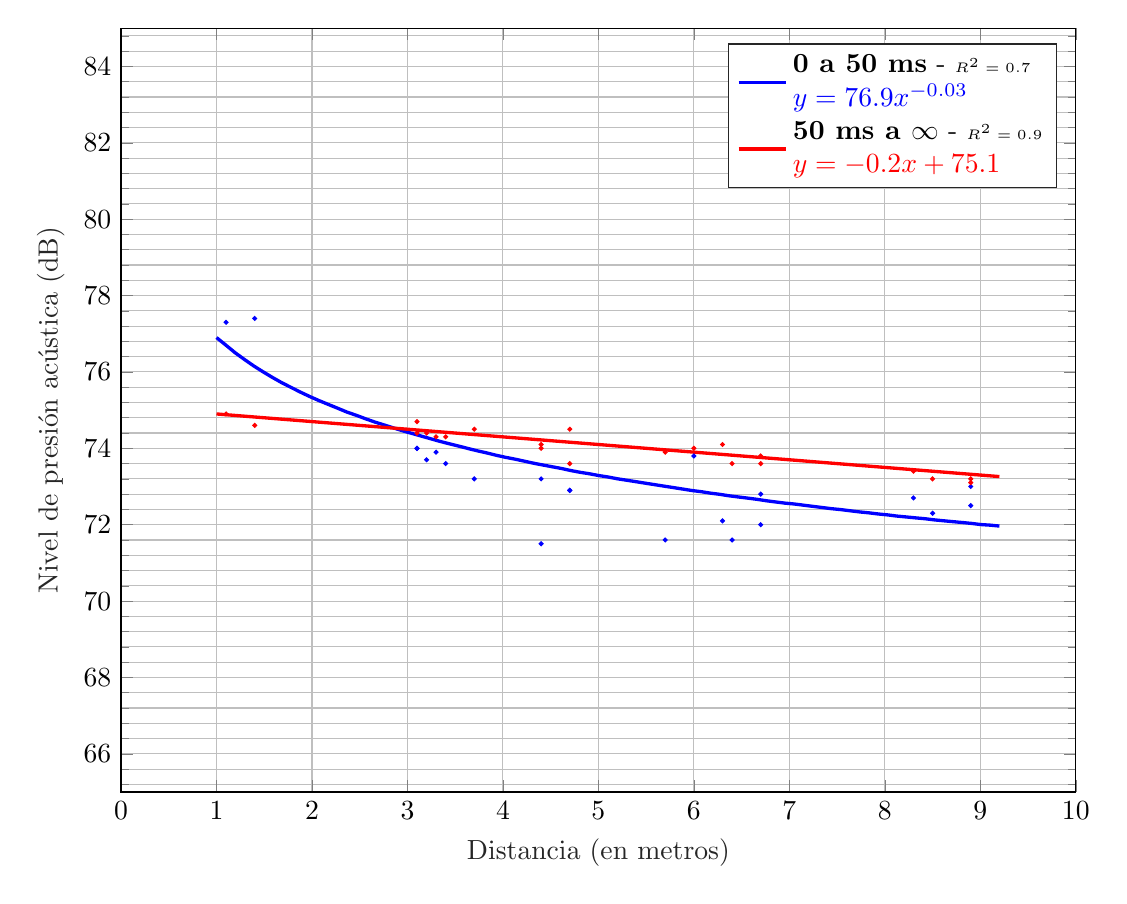
\begin{tikzpicture}

\begin{axis}[%
width=\textwidth,
height=0.8\textwidth,
at={(0\textwidth,0\textwidth)},
scale only axis,
xmin=0,
xmax=10,
xlabel style={font=\color{white!15!black}},
xlabel={Distancia (en metros)},
ymin=65,
ymax=85,
xmajorgrids,
xminorgrids,
ymajorgrids,
yminorgrids,
minor y tick num= 4,
ylabel style={font=\color{white!15!black}},
ylabel={Nivel de presión acústica (dB)},
axis background/.style={fill=white},
%xmajorgrids,
%xminorgrids,
%ymajorgrids,
%yminorgrids,
legend style={legend cell align=left, align=left, draw=white!15!black}
]
\addplot[color=blue,domain=1:9.2, samples=85,line width=1.2]{76.9*x^(-0.03)};
\addlegendentry{\textbf{0 a 50 ms} - \tiny{$R^2 = 0.7$}\\$\color{blue}y = 76.9·x^{-0.03}$}

\addplot[color=red,domain=1:9.2, samples=85,line width=1.2]{-0.20*x+75.10};
\addlegendentry{\textbf{50 ms a $\infty$} - \tiny{$R^2 = 0.9$}\\$\color{red}y = -0.2·x+75.1$}

% Puntos
\addplot [color=blue, only marks,mark size=0.7pt]
  table[row sep=crcr]{%
  8.9	72.5\\
6.7	72.0\\
4.7	72.9\\
3.3	73.9\\
3.1	74.0\\
4.4	73.2\\
6.4	71.6\\
8.3	72.7\\
6.0	73.8\\
3.7	73.2\\
1.4	77.4\\
1.1	77.3\\
3.4	73.6\\
5.7	71.6\\
8.9	73.0\\
6.7	72.8\\
4.7	72.9\\
3.2	73.7\\
3.1	74.0\\
4.4	71.5\\
6.3	72.1\\
8.5	72.3\\
  };
  
  \addplot [color=red, only marks,mark size=0.7pt]
  table[row sep=crcr]{%
  8.9	73.2\\
6.7	73.8\\
4.7	74.5\\
3.3	74.3\\
3.1	74.7\\
4.4	74.1\\
6.4	73.6\\
8.3	73.4\\
6.0	74.0\\
3.7	74.5\\
1.4	74.6\\
1.1	74.9\\
3.4	74.3\\
5.7	73.9\\
8.9	73.1\\
6.7	73.6\\
4.7	73.6\\
3.2	74.4\\
3.1	74.4\\
4.4	74.0\\
6.3	74.1\\
8.5	73.2\\
  };
\end{axis}
\end{tikzpicture}%%
    }
    \caption{Fuente en el centro}%
    \end{subfigure}
    \caption{Campos acústicos en el aula OP/S003 sin mobiliario. 22 puntos de medida}
    \label{graf:opnomob}%
\end{figure}


%%%%%
%%%%% MAPAS OPTICA
%%%%%

\begin{figure}[H]
    \centering%
        {\scalefont{0.8}%
    %%%%%%%%%%%%%%%%%%%%%%%%%%%%%%%%%%%%%%%%%%%%%%%%%%%%%%%%%%%%%%%%%%%%%%%%
% Escuela Politécnica Superior de la Universidad de Alicante
% Realizado por: Jose Manuel Requena Plens
% Contacto: info@jmrplens.com / Telegram:@jmrplens
%%%%%%%%%%%%%%%%%%%%%%%%%%%%%%%%%%%%%%%%%%%%%%%%%%%%%%%%%%%%%%%%%%%%%%%%


\begin{tikzpicture}
\begin{groupplot}[
      group style = {
        group size = 2 by 1,
        horizontal sep = 2cm,
      },
      view = {0}{90},
      colormap name=jet,
      ]
      
  % GRAFICA 1
  \nextgroupplot[
  	width=0.45\textwidth,
  	view={0}{90},
	xlabel style={font=\color{white!15!black}},
	xlabel={Lx (m)},
	ylabel style={font=\color{white!15!black}},
	ylabel={Ly (m)},
	axis equal image=true,
	point meta min=69,
	point meta max=82,
%          colorbar horizontal,
%          colorbar style = {
%          	xlabel={Nivel de presión acústica (dB)},
%            at={(rel axis cs: 1.1,-0.3)},
%            anchor=south,
%            height=3mm,
%            axis line style={draw=none}
%          },
	colorbar,
          colorbar style = {
          	ylabel={SPL (dB)},
            at={(rel axis cs: 1.11,1)},
            ylabel style={font=\normalfont,at={(rel axis cs: -2.8,0.5)}},
            %anchor=south,
            width=2mm,
            axis line style={draw=none}
          },
	]

	\addplot3 [
    	surf,
    	shader=interp,
    	mesh/cols=51,mesh/ordering=y varies,
	]
    	table {archivos/graficastikz/OpLlenaEsquinaUtilMalla.dat};
    	
    	
    % Imprime la fuente
\addplot[only marks,mark=*,white,mark size=3pt,mark options={fill=black}]
    	coordinates {
    	(0.4,0.6)
    	};	
    	
    % Imprime los receptores
\addplot[only marks,mark=triangle*,white, mark size=2pt, mark options={fill=blue}]
    	coordinates {
    	(0.90,1.40)
		(1.90,1.40)
		(2.90,1.40)
		(4.00,1.40)
		(5.10,1.40)
		(6.10,1.40)
		(7.10,1.40)
		(8.10,1.40)
		(9.30,1.40)
		(10.2,1.40)
		(11.3,1.40)
		(12.3,1.40)
		(13.3,1.40)
		(14.3,1.40)
		(15.2,1.40)
		(16.2,1.40)
		(0.90,5.30)
		(1.90,5.30)
		(2.90,5.30)
		(4.00,5.30)
		(5.10,5.30)
		(6.10,5.30)
		(7.10,5.30)
		(8.10,5.30)
		(9.30,5.30)
		(10.2,5.30)
		(11.3,5.30)
		(12.3,5.30)
		(13.3,5.30)
		(14.3,5.30)
		(15.2,5.30)
		(16.2,5.30)
		(0.90,7.60)
		(1.90,7.60)
		(2.90,7.60)
		(4.00,7.60)
		(5.10,7.60)
		(6.10,7.60)
		(7.10,7.60)
		(8.10,7.60)
		(9.30,7.60)
		(10.2,7.60)
		(11.3,7.60)
		(12.3,7.60)
		(13.3,7.60)
		(14.3,7.60)
		(15.2,7.60)
		(16.2,7.60)
		};	
		
	% GRAFICA 2
  \nextgroupplot[
  	width=0.45\textwidth,
  	view={0}{90},
	xlabel style={font=\color{white!15!black}},
	xlabel={Lx (m)},
	ylabel style={font=\color{white!15!black}},
	ylabel={Ly (m)},
	axis equal image=true,
	point meta min=69,
	point meta max=82,
	yticklabel pos=right,
	]
	
	\addplot3 [
    	surf,
    	shader=interp,
    	mesh/cols=51,mesh/ordering=y varies,
	]
    	table {archivos/graficastikz/OpLlenaCentroUtilMalla.dat};
    	
    	
    % Imprime la fuente
\addplot[only marks,mark=*,white,mark size=3pt,mark options={fill=black}]
    	coordinates {
    	(9.4,4.6)
    	};	
    	
    % Imprime los receptores
\addplot[only marks,mark=triangle*,white, mark size=2pt, mark options={fill=blue}]
    	coordinates {
    	(0.90,1.40)
		(1.90,1.40)
		(2.90,1.40)
		(4.00,1.40)
		(5.10,1.40)
		(6.10,1.40)
		(7.10,1.40)
		(8.10,1.40)
		(9.30,1.40)
		(10.2,1.40)
		(11.3,1.40)
		(12.3,1.40)
		(13.3,1.40)
		(14.3,1.40)
		(15.2,1.40)
		(16.2,1.40)
		(0.90,5.30)
		(1.90,5.30)
		(2.90,5.30)
		(4.00,5.30)
		(5.10,5.30)
		(6.10,5.30)
		(7.10,5.30)
		(8.10,5.30)
		(9.30,5.30)
		(10.2,5.30)
		(11.3,5.30)
		(12.3,5.30)
		(13.3,5.30)
		(14.3,5.30)
		(15.2,5.30)
		(16.2,5.30)
		(0.90,7.60)
		(1.90,7.60)
		(2.90,7.60)
		(4.00,7.60)
		(5.10,7.60)
		(6.10,7.60)
		(7.10,7.60)
		(8.10,7.60)
		(9.30,7.60)
		(10.2,7.60)
		(11.3,7.60)
		(12.3,7.60)
		(13.3,7.60)
		(14.3,7.60)
		(15.2,7.60)
		(16.2,7.60)
		};	
\end{groupplot}

\end{tikzpicture}%%
    }
    \caption{Campos útiles (0 a 50ms) para ambas posiciones de fuente en el aula OP/S003 con mobiliario. Las fuentes (círculos) y los 48 puntos de medida (triángulos)}
    \label{graf:mapaoputilcon}%
\end{figure}


\begin{figure}[H]
    \centering%
        {\scalefont{0.8}%
    %%%%%%%%%%%%%%%%%%%%%%%%%%%%%%%%%%%%%%%%%%%%%%%%%%%%%%%%%%%%%%%%%%%%%%%%
% Escuela Politécnica Superior de la Universidad de Alicante
% Realizado por: Jose Manuel Requena Plens
% Contacto: info@jmrplens.com / Telegram:@jmrplens
%%%%%%%%%%%%%%%%%%%%%%%%%%%%%%%%%%%%%%%%%%%%%%%%%%%%%%%%%%%%%%%%%%%%%%%%


\begin{tikzpicture}

\begin{groupplot}[
      group style = {
        group size = 2 by 1,
        horizontal sep = 2cm,
      },
      view = {0}{90},
      colormap name=jet,
      ]
      
  % GRAFICA 1
  \nextgroupplot[
  	width=0.45\textwidth,
  	view={0}{90},
	xlabel style={font=\color{white!15!black}},
	xlabel={Lx (m)},
	ylabel style={font=\color{white!15!black}},
	ylabel={Ly (m)},
	axis equal image=true,
	point meta min=70,
	point meta max=86,
%          colorbar horizontal,
%          colorbar style = {
%          	xlabel={Nivel de presión acústica (dB)},
%            at={(rel axis cs: 1.1,-0.3)},
%            anchor=south,
%            height=3mm,
%            axis line style={draw=none}
%          },
	colorbar,
	colorbar style = {
		ylabel={SPL (dB)},
	at={(rel axis cs: 1.11,1)},
	ylabel style={font=\normalfont,at={(rel axis cs: -2.8,0.5)}},
	%anchor=south,
	width=2mm,
	axis line style={draw=none}
	},
	]

	\addplot3 [
    	surf,
    	shader=interp,
    	mesh/cols=51,mesh/ordering=y varies,
	]
    	table {archivos/graficastikz/OpVaciaEsquinaUtilMalla.dat};
    	
    	
    % Imprime la fuente
\addplot[only marks,mark=*,white,mark size=3pt,mark options={fill=black}]
    	coordinates {
    	(0.4,0.6)
    	};	
    	
    % Imprime los receptores
\addplot[only marks,mark=triangle*,white, mark size=2pt, mark options={fill=blue}]
    	coordinates {
    	(1,1.60)
		(3.10,1.60)
		(5.70,1.60)
		(8,1.60)
		(10.4,1.60)
		(12.8,1.60)
		(15.4,1.60)
		(1,4.50)
		(3.10,4.50)
		(5.70,4.50)
		(8,4.50)
		(10.4,4.50)
		(12.8,4.50)
		(15.4,4.50)
		(1,7.60)
		(3.10,7.60)
		(5.70,7.60)
		(8,7.60)
		(10.4,7.60)
		(12.8,7.60)
		(15.4,7.60)
		(17.7,7.60)
		};	
		
	% GRAFICA 2
  \nextgroupplot[
  	width=0.45\textwidth,
  	view={0}{90},
	xlabel style={font=\color{white!15!black}},
	xlabel={Lx (m)},
	ylabel style={font=\color{white!15!black}},
	ylabel={Ly (m)},
	axis equal image=true,
	point meta min=70,
	point meta max=86,
	yticklabel pos=right,
	]
	
	\addplot3 [
    	surf,
    	shader=interp,
    	mesh/cols=51,mesh/ordering=y varies,
	]
    	table {archivos/graficastikz/OpVaciaCentroUtilMalla.dat};
    	
    	
    % Imprime la fuente
\addplot[only marks,mark=*,white,mark size=3pt,mark options={fill=black}]
    	coordinates {
    	(9.4,4.6)
    	};	
    	
    % Imprime los receptores
\addplot[only marks,mark=triangle*,white, mark size=2pt, mark options={fill=blue}]
    	coordinates {
    	(1,1.60)
		(3.10,1.60)
		(5.70,1.60)
		(8,1.60)
		(10.4,1.60)
		(12.8,1.60)
		(15.4,1.60)
		(1,4.50)
		(3.10,4.50)
		(5.70,4.50)
		(8,4.50)
		(10.4,4.50)
		(12.8,4.50)
		(15.4,4.50)
		(1,7.60)
		(3.10,7.60)
		(5.70,7.60)
		(8,7.60)
		(10.4,7.60)
		(12.8,7.60)
		(15.4,7.60)
		(17.7,7.60)
		};	
\end{groupplot}

\end{tikzpicture}%%
    }
    \caption{Campos útiles (0 a 50ms) para ambas posiciones de fuente en el aula OP/S003 sin mobiliario. Las fuentes (círculos) y los 48 puntos de medida (triángulos)}
    \label{graf:mapaoputilsin}%
\end{figure}



\begin{figure}[H]
    \centering%
        {\scalefont{0.8}%
    %%%%%%%%%%%%%%%%%%%%%%%%%%%%%%%%%%%%%%%%%%%%%%%%%%%%%%%%%%%%%%%%%%%%%%%%
% Escuela Politécnica Superior de la Universidad de Alicante
% Realizado por: Jose Manuel Requena Plens
% Contacto: info@jmrplens.com / Telegram:@jmrplens
%%%%%%%%%%%%%%%%%%%%%%%%%%%%%%%%%%%%%%%%%%%%%%%%%%%%%%%%%%%%%%%%%%%%%%%%

\begin{tikzpicture}

\begin{groupplot}[
      group style = {
        group size = 2 by 1,
        horizontal sep = 2cm,
      },
      view = {0}{90},
      colormap name=jet,
      ]
      
  % GRAFICA 1
  \nextgroupplot[
  	width=0.45\textwidth,
  	view={0}{90},
	xlabel style={font=\color{white!15!black}},
	xlabel={Lx (m)},
	ylabel style={font=\color{white!15!black}},
	ylabel={Ly (m)},
	axis equal image=true,
	point meta min=71,
	point meta max=76,
%          colorbar horizontal,
%          colorbar style = {
%          	xlabel={Nivel de presión acústica (dB)},
%            at={(rel axis cs: 1.1,-0.3)},
%            anchor=south,
%            height=3mm,
%            axis line style={draw=none}
%          },
colorbar,
          colorbar style = {
          	ylabel={SPL (dB)},
            at={(rel axis cs: 1.11,1)},
            ylabel style={font=\normalfont,at={(rel axis cs: -2.8,0.5)}},
            %anchor=south,
            width=2mm,
            axis line style={draw=none}
          },
	]

	\addplot3 [
    	surf,
    	shader=interp,
    	mesh/cols=51,mesh/ordering=y varies,
	]
    	table {archivos/graficastikz/OpLlenaEsquinaPerjudicialMalla.dat};
    	
    	
    % Imprime la fuente
\addplot[only marks,mark=*,white,mark size=3pt,mark options={fill=black}]
    	coordinates {
    	(0.4,0.6)
    	};	
    	
    % Imprime los receptores
\addplot[only marks,mark=triangle*,white, mark size=2pt, mark options={fill=blue}]
    	coordinates {
    	(0.90,1.40)
		(1.90,1.40)
		(2.90,1.40)
		(4.00,1.40)
		(5.10,1.40)
		(6.10,1.40)
		(7.10,1.40)
		(8.10,1.40)
		(9.30,1.40)
		(10.2,1.40)
		(11.3,1.40)
		(12.3,1.40)
		(13.3,1.40)
		(14.3,1.40)
		(15.2,1.40)
		(16.2,1.40)
		(0.90,5.30)
		(1.90,5.30)
		(2.90,5.30)
		(4.00,5.30)
		(5.10,5.30)
		(6.10,5.30)
		(7.10,5.30)
		(8.10,5.30)
		(9.30,5.30)
		(10.2,5.30)
		(11.3,5.30)
		(12.3,5.30)
		(13.3,5.30)
		(14.3,5.30)
		(15.2,5.30)
		(16.2,5.30)
		(0.90,7.60)
		(1.90,7.60)
		(2.90,7.60)
		(4.00,7.60)
		(5.10,7.60)
		(6.10,7.60)
		(7.10,7.60)
		(8.10,7.60)
		(9.30,7.60)
		(10.2,7.60)
		(11.3,7.60)
		(12.3,7.60)
		(13.3,7.60)
		(14.3,7.60)
		(15.2,7.60)
		(16.2,7.60)
		};	
		
	% GRAFICA 2
  \nextgroupplot[
  	width=0.45\textwidth,
  	view={0}{90},
	xlabel style={font=\color{white!15!black}},
	xlabel={Lx (m)},
	ylabel style={font=\color{white!15!black}},
	ylabel={Ly (m)},
	axis equal image=true,
	point meta min=71,
	point meta max=76,
	yticklabel pos=right,
	]
	
	\addplot3 [
    	surf,
    	shader=interp,
    	mesh/cols=51,mesh/ordering=y varies,
	]
    	table {archivos/graficastikz/OpLlenaCentroPerjudicialMalla.dat};
    	
    	
    % Imprime la fuente
\addplot[only marks,mark=*,white,mark size=3pt,mark options={fill=black}]
    	coordinates {
    	(9.4,4.6)
    	};	
    	
    % Imprime los receptores
\addplot[only marks,mark=triangle*,white, mark size=2pt, mark options={fill=blue}]
    	coordinates {
    	(0.90,1.40)
		(1.90,1.40)
		(2.90,1.40)
		(4.00,1.40)
		(5.10,1.40)
		(6.10,1.40)
		(7.10,1.40)
		(8.10,1.40)
		(9.30,1.40)
		(10.2,1.40)
		(11.3,1.40)
		(12.3,1.40)
		(13.3,1.40)
		(14.3,1.40)
		(15.2,1.40)
		(16.2,1.40)
		(0.90,5.30)
		(1.90,5.30)
		(2.90,5.30)
		(4.00,5.30)
		(5.10,5.30)
		(6.10,5.30)
		(7.10,5.30)
		(8.10,5.30)
		(9.30,5.30)
		(10.2,5.30)
		(11.3,5.30)
		(12.3,5.30)
		(13.3,5.30)
		(14.3,5.30)
		(15.2,5.30)
		(16.2,5.30)
		(0.90,7.60)
		(1.90,7.60)
		(2.90,7.60)
		(4.00,7.60)
		(5.10,7.60)
		(6.10,7.60)
		(7.10,7.60)
		(8.10,7.60)
		(9.30,7.60)
		(10.2,7.60)
		(11.3,7.60)
		(12.3,7.60)
		(13.3,7.60)
		(14.3,7.60)
		(15.2,7.60)
		(16.2,7.60)
		};	
\end{groupplot}

\end{tikzpicture}%%
    }
    \caption{Campos perjudiciales (50 ms a $\infty$) para ambas posiciones de fuente en el aula OP/S003 con mobiliario. Las fuentes (círculos) y los 48 puntos de medida (triángulos)}
    \label{graf:mapaopperjudicialcon}%
\end{figure}

\begin{figure}[H]
    \centering%
        {\scalefont{0.8}%
    %%%%%%%%%%%%%%%%%%%%%%%%%%%%%%%%%%%%%%%%%%%%%%%%%%%%%%%%%%%%%%%%%%%%%%%%
% Escuela Politécnica Superior de la Universidad de Alicante
% Realizado por: Jose Manuel Requena Plens
% Contacto: info@jmrplens.com / Telegram:@jmrplens
%%%%%%%%%%%%%%%%%%%%%%%%%%%%%%%%%%%%%%%%%%%%%%%%%%%%%%%%%%%%%%%%%%%%%%%%

\begin{tikzpicture}

\begin{groupplot}[
      group style = {
        group size = 2 by 1,
        horizontal sep = 2cm,
      },
      view = {0}{90},
      colormap name=jet,
      ]
      
  % GRAFICA 1
  \nextgroupplot[
  	width=0.45\textwidth,
  	view={0}{90},
	xlabel style={font=\color{white!15!black}},
	xlabel={Lx (m)},
	ylabel style={font=\color{white!15!black}},
	ylabel={Ly (m)},
	axis equal image=true,
	point meta min=71,
	point meta max=76,
          colorbar,
          colorbar style = {
          	ylabel={SPL (dB)},
            at={(rel axis cs: 1.11,1)},
            ylabel style={font=\normalfont,at={(rel axis cs: -2.8,0.5)}},
            %anchor=south,
            width=2mm,
            axis line style={draw=none}
          },
	]

	\addplot3 [
    	surf,
    	shader=interp,
    	mesh/cols=51,mesh/ordering=y varies,
	]
    	table {archivos/graficastikz/OpVaciaEsquinaPerjudicialMalla.dat};
    	
    	
    % Imprime la fuente
\addplot[only marks,mark=*,white,mark size=3pt,mark options={fill=black}]
    	coordinates {
    	(0.4,0.6)
    	};	
    	
    % Imprime los receptores
\addplot[only marks,mark=triangle*,white, mark size=2pt, mark options={fill=blue}]
    	coordinates {
    	(1,1.60)
		(3.10,1.60)
		(5.70,1.60)
		(8,1.60)
		(10.4,1.60)
		(12.8,1.60)
		(15.4,1.60)
		(1,4.50)
		(3.10,4.50)
		(5.70,4.50)
		(8,4.50)
		(10.4,4.50)
		(12.8,4.50)
		(15.4,4.50)
		(1,7.60)
		(3.10,7.60)
		(5.70,7.60)
		(8,7.60)
		(10.4,7.60)
		(12.8,7.60)
		(15.4,7.60)
		(17.7,7.60)
		};	
		
	% GRAFICA 2
  \nextgroupplot[
  	width=0.45\textwidth,
  	view={0}{90},
	xlabel style={font=\color{white!15!black}},
	xlabel={Lx (m)},
	ylabel style={font=\color{white!15!black}},
	ylabel={Ly (m)},
	axis equal image=true,
	point meta min=71,
	point meta max=76,
	yticklabel pos=right,
	]
	
	\addplot3 [
    	surf,
    	shader=interp,
    	mesh/cols=51,mesh/ordering=y varies,
	]
    	table {archivos/graficastikz/OpVaciaCentroPerjudicialMalla.dat};
    	
    	
    % Imprime la fuente
\addplot[only marks,mark=*,white,mark size=3pt,mark options={fill=black}]
    	coordinates {
    	(9.4,4.6)
    	};	
    	
    % Imprime los receptores
\addplot[only marks,mark=triangle*,white, mark size=2pt, mark options={fill=blue}]
    	coordinates {
    	(1,1.60)
		(3.10,1.60)
		(5.70,1.60)
		(8,1.60)
		(10.4,1.60)
		(12.8,1.60)
		(15.4,1.60)
		(1,4.50)
		(3.10,4.50)
		(5.70,4.50)
		(8,4.50)
		(10.4,4.50)
		(12.8,4.50)
		(15.4,4.50)
		(1,7.60)
		(3.10,7.60)
		(5.70,7.60)
		(8,7.60)
		(10.4,7.60)
		(12.8,7.60)
		(15.4,7.60)
		(17.7,7.60)
		};	
\end{groupplot}

\end{tikzpicture}%%
    }
    \caption{Campos perjudiciales (50 ms a $\infty$) para ambas posiciones de fuente en el aula OP/S003 sin mobiliario. Las fuentes (círculos) y los 48 puntos de medida (triángulos)}
    \label{graf:mapaopperjudicialsin}%
\end{figure}

Debido al método de extrapolación en las zonas entre los puntos de recepción y los límites del recinto se producen ciertos artefactos como los que aparecen en el lado derecho de ambos mapas de la figura \ref{graf:mapaopperjudicialcon}.

\subsection{Aula EP/0-26M}

El aula EP/0-26M está ubicada en la planta baja de la Escuela Politécnica Superior IV de la Universidad de Alicante.

\begin{figure}[ht]
    \centering
    \begin{subfigure}[b]{0.4\textwidth}
    	\centering
        \includegraphics[width=0.9\linewidth]{archivos/eps1.jpg}
    \end{subfigure}
    ~ % Añadir el espacio deseado, si se deja la linea en blanco la siguiente subfigura ira en una nueva linea
    \begin{subfigure}[b]{0.4\textwidth}
    	\centering
        \includegraphics[width=0.9\linewidth]{archivos/eps2.jpg}
    \end{subfigure}
    \caption{Aula EP/0-26M.}\label{fotoseps}
\end{figure}
\FloatBarrier 

Los detalles del recinto son:
\begin{itemize}
\itemsep0em
  \item \textbf{Dimensiones:} 11.9x7.1x2.7 $m$.
  \item \textbf{Volumen:} \textasciitilde230 $m^3$.
  \item \textbf{Superficie recinto:} \textasciitilde270 $m^2$.
  \item \textbf{Número de mesas:} 32 (dimensiones 1.20x0.45 $m$).
  \item \textbf{Número de sillas:} 64 (dimensiones 0.44x0.51 $m$).
\end{itemize}

Los materiales y sus absorciones según la literatura son:
\begin{itemize}
\itemsep0em
  \item Cerramientos transversales y del lateral con ventana, de hormigón armado: $\overline{\alpha}\approx0.02$.
  \item Cerramientos laterales de placa de yeso pintado: $\overline{\alpha}\approx0.03$.
  \item Suelo de terrazo: $\overline{\alpha}\approx0.02$.
  \item Techo registrable de escayola: $\overline{\alpha}\approx0.10$.
  \item Mobiliario de paneles multilaminares: $\overline{\alpha}\approx0.03$.
  \item Ventanales: $\overline{\alpha}\approx0.03$
\end{itemize}

Las medidas del tiempo de reverberación por bandas de octava son:

\begin{table}[ht]
\centering
{\scalefont{0.9}
\begin{tabular}{@{}lccccccc@{}}
\toprule
Frecuencia (Hz) & 125 & 250 & 500 & 1000 & 2000 & 4000 & 8000 \\ \midrule
$T_{60}$ Con mobiliario (s) & 1.34 & 1.50 & 1.45 & 1.28 & 1.17 & 1.05 & 0.76 \\
$T_{60}$ Sin mobiliario (s) & 1.31 & 1.57 & 1.57 & 1.43 & 1.30 & 1.16 & 0.84 \\ \bottomrule
\end{tabular}
}
\caption{Tiempos de reverberación obtenidos en el aula EP/0-26M por banda de octava, con y sin mobiliario.}
\label{tab:reveps}
\end{table}

Las posiciones de los receptores y las fuentes se muestran en las figuras \ref{im:receptoreseps}, un total de 30 receptores y 2 fuentes.

\begin{figure}[ht]
    \centering
    \begin{subfigure}[b]{0.4\textwidth}
    	\centering
        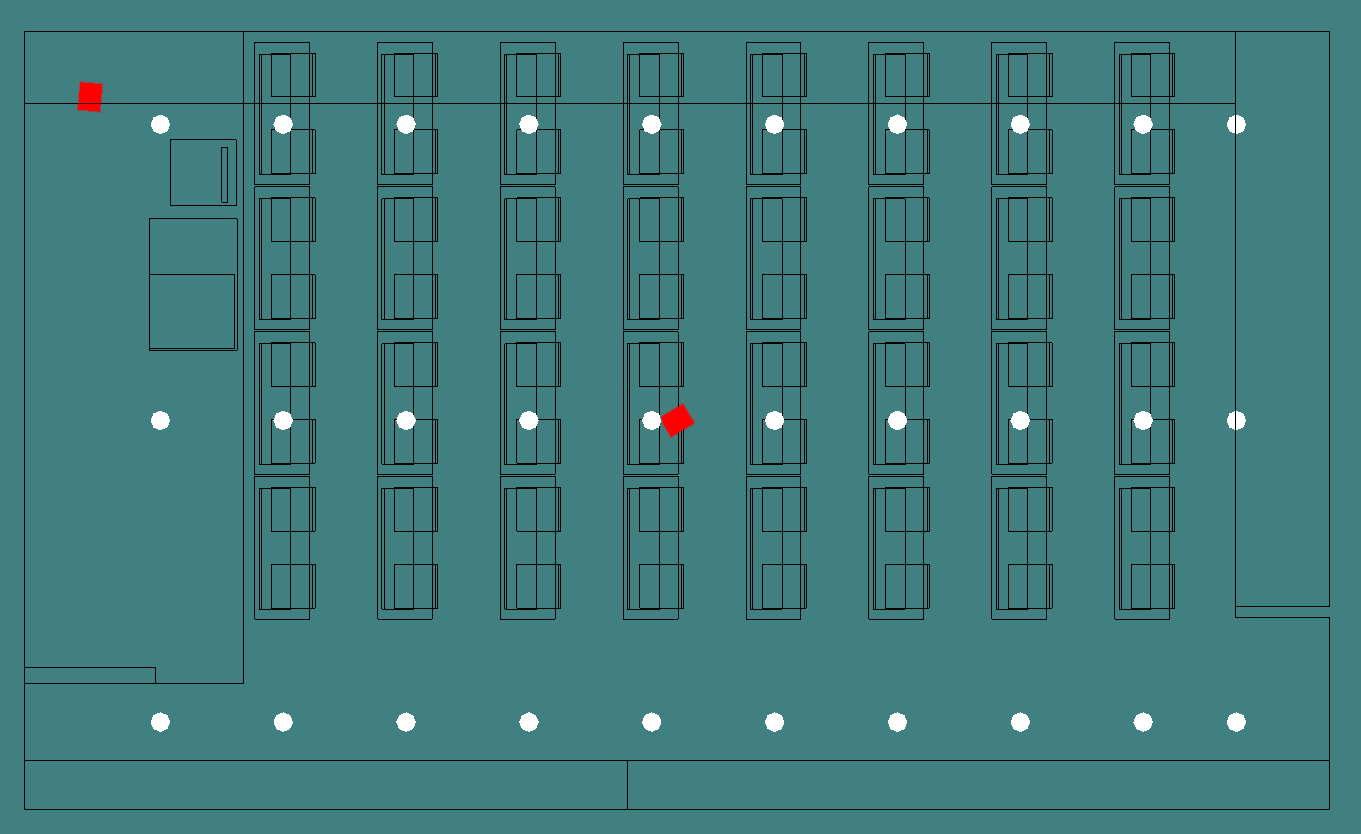
\includegraphics[width=0.9\textwidth]{archivos/receptoreseps.png}
        \caption{Con mobiliario.}
    \end{subfigure}
    ~ % Añadir el espacio deseado, si se deja la linea en blanco la siguiente subfigura ira en una nueva linea
    \begin{subfigure}[b]{0.4\textwidth}
    	\centering
        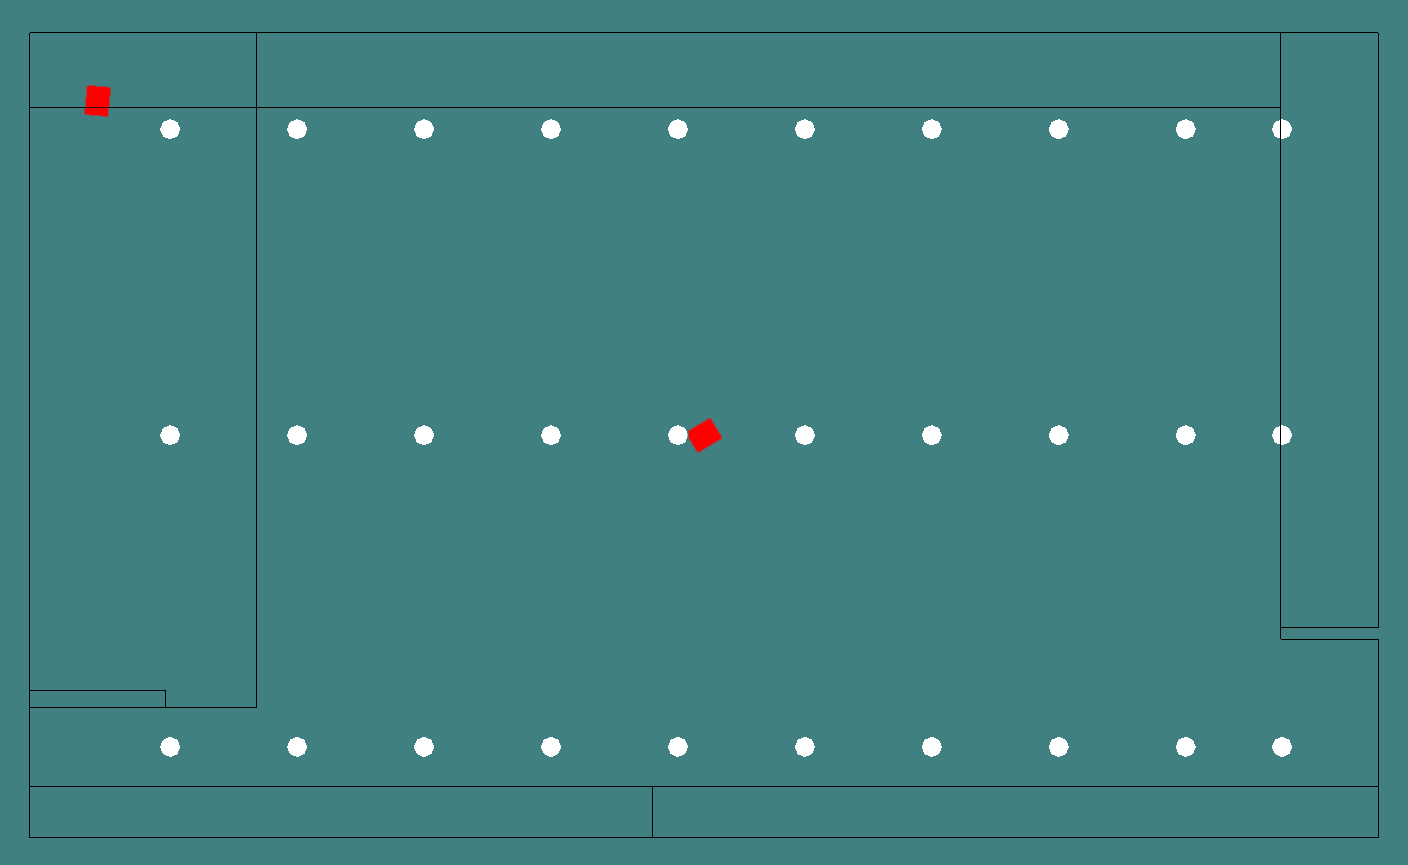
\includegraphics[width=0.9\linewidth]{archivos/receptoresepsv.png}
        \caption{Sin mobiliario.}
    \end{subfigure}
    \caption{Puntos de recepción (círculos blancos) y fuentes (rectángulos rojos) en aula EP/0-26M.}\label{im:receptoreseps}
\end{figure}
\FloatBarrier 


\begin{figure}[ht]
    \begin{subfigure}[b]{0.4\textwidth}
    	\centering%
         {\scalefont{0.8}%
    %%%%%%%%%%%%%%%%%%%%%%%%%%%%%%%%%%%%%%%%%%%%%%%%%%%%%%%%%%%%%%%%%%%%%%%%
% Escuela Politécnica Superior de la Universidad de Alicante
% Realizado por: Jose Manuel Requena Plens
% Contacto: info@jmrplens.com / Telegram:@jmrplens
%%%%%%%%%%%%%%%%%%%%%%%%%%%%%%%%%%%%%%%%%%%%%%%%%%%%%%%%%%%%%%%%%%%%%%%%


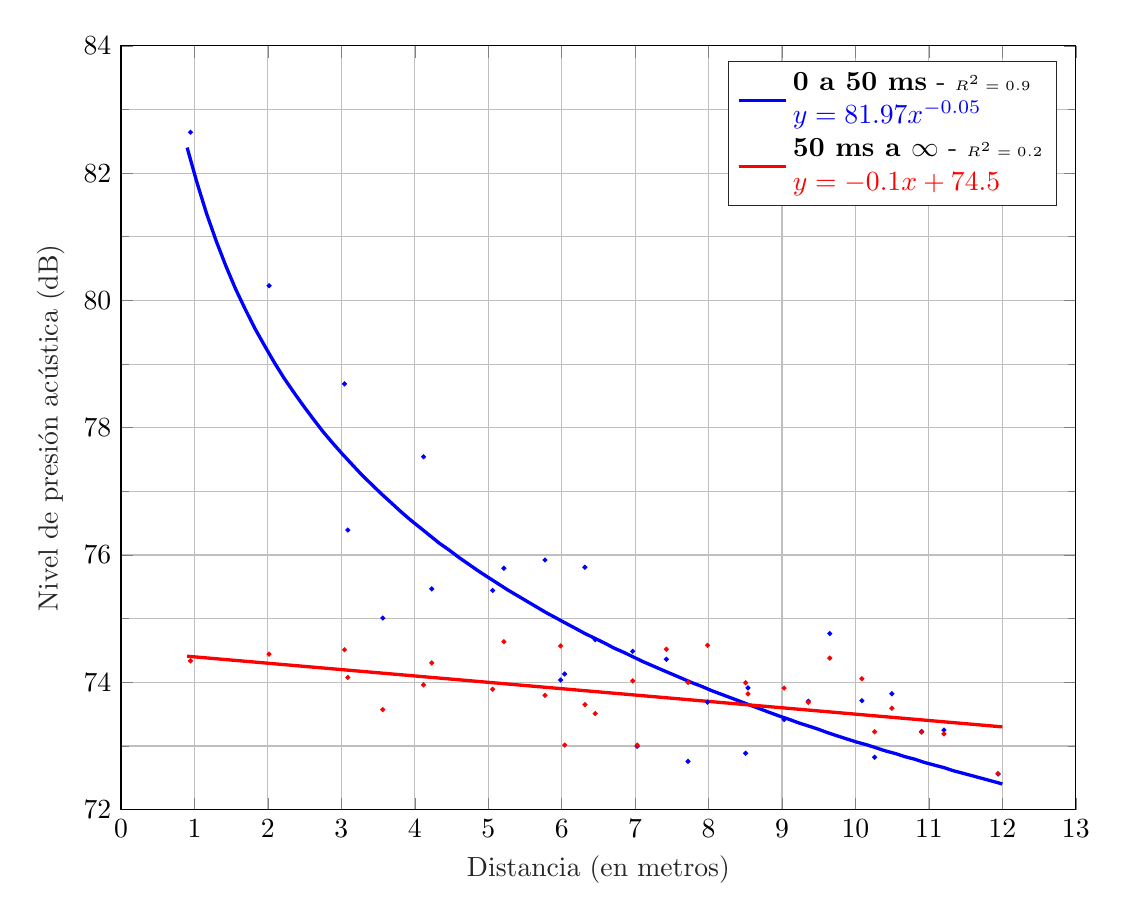
\begin{tikzpicture}

\begin{axis}[%
width=\textwidth,
height=0.8\textwidth,
at={(0\textwidth,0\textwidth)},
scale only axis,
xmin=0,
xmax=13,
xlabel style={font=\color{white!15!black}},
xlabel={Distancia (en metros)},
ymin=72,
ymax=84,
xmajorgrids,
xminorgrids,
ymajorgrids,
yminorgrids,
minor y tick num= 1,
ylabel style={font=\color{white!15!black}},
ylabel={Nivel de presión acústica (dB)},
axis background/.style={fill=white},
legend style={legend cell align=left, align=left, draw=white!15!black}
]
\addplot [color=blue, only marks,mark size=0.7pt, forget plot]
  table[row sep=crcr]{%
0.945832966226064	82.6420079958914\\
2.0155892438689	80.2303554003687\\
3.04292622322659	78.6881045727944\\
3.08781476128345	76.3922767253641\\
3.56407070636934	75.0100820613083\\
4.11885906532379	77.543416910588\\
4.23076825174815	75.4693527412033\\
5.0601383380299	75.444066602597\\
5.21338661524349	75.7915413606487\\
5.7725297747175	75.9216852693002\\
5.98493107729738	74.0366131016921\\
6.04070360140274	74.1312005354213\\
6.31685048105462	75.8077293987195\\
6.45653932071973	74.6715272292603\\
6.96725196903341	74.4875231200194\\
7.02797979507625	72.99559772715\\
7.42526767194288	74.3627070297666\\
7.72055049850721	72.7576960941599\\
7.98590007450632	73.6889279610953\\
8.5047104595042	72.8855286933151\\
8.53670896774629	73.9130300559927\\
9.02858792946051	73.4166836406291\\
9.35746226281464	73.702884884372\\
9.65012953280939	74.7664519770778\\
10.0878639959111	73.71153847285\\
10.2617201287114	72.822938510167\\
10.4960706933595	73.8196487744781\\
10.8998853204976	73.227376539976\\
11.2050211958747	73.2501558174068\\
11.9413148354777	72.5594130132974\\
};
\addplot[color=blue,domain=0.9:12, samples=85,line width=1.2]{81.97*x^(-0.05)};
\addlegendentry{\textbf{0 a 50 ms} - \tiny{$R^2 = 0.9$}\\$\color{blue}y = 81.97·x^{-0.05}$}

\addplot [color=red, only marks,mark size=0.7pt, forget plot]
  table[row sep=crcr]{%
0.945832966226064	74.3367942916818\\
2.0155892438689	74.4428555138378\\
3.04292622322659	74.511850056859\\
3.08781476128345	74.0768454974658\\
3.56407070636934	73.570968193684\\
4.11885906532379	73.960193320587\\
4.23076825174815	74.3058561007808\\
5.0601383380299	73.8906487606386\\
5.21338661524349	74.638243792516\\
5.7725297747175	73.793741140568\\
5.98493107729738	74.5716721982254\\
6.04070360140274	73.0144941684959\\
6.31685048105462	73.6493891472023\\
6.45653932071973	73.509586766673\\
6.96725196903341	74.0237029187056\\
7.02797979507625	73.0128244006444\\
7.42526767194288	74.5199342918284\\
7.72055049850721	73.9989506580923\\
7.98590007450632	74.5821265722156\\
8.5047104595042	73.9925438985215\\
8.53670896774629	73.8193785231492\\
9.02858792946051	73.9085522734068\\
9.35746226281464	73.6859259436621\\
9.65012953280939	74.3803174126395\\
10.0878639959111	74.0555050161735\\
10.2617201287114	73.2230389538318\\
10.4960706933595	73.5932649217609\\
10.8998853204976	73.2166557384589\\
11.2050211958747	73.1901137726248\\
11.9413148354777	72.5672282318972\\
};
\addplot[color=red,domain=0.9:12, samples=85,line width=1.2]{-0.1*x+74.5};
\addlegendentry{\textbf{50 ms a $\infty$} - \tiny{$R^2 = 0.2$}\\$\color{red}y = -0.1·x+74.5$}

\end{axis}
\end{tikzpicture}%%
    }
    \caption{Fuente en la esquina}%
    \end{subfigure}%
    \hspace{1.9cm}%
    \begin{subfigure}[b]{0.4\textwidth}%
    	\centering%
        {\scalefont{0.8}%
    %%%%%%%%%%%%%%%%%%%%%%%%%%%%%%%%%%%%%%%%%%%%%%%%%%%%%%%%%%%%%%%%%%%%%%%%
% Escuela Politécnica Superior de la Universidad de Alicante
% Realizado por: Jose Manuel Requena Plens
% Contacto: info@jmrplens.com / Telegram:@jmrplens
%%%%%%%%%%%%%%%%%%%%%%%%%%%%%%%%%%%%%%%%%%%%%%%%%%%%%%%%%%%%%%%%%%%%%%%%

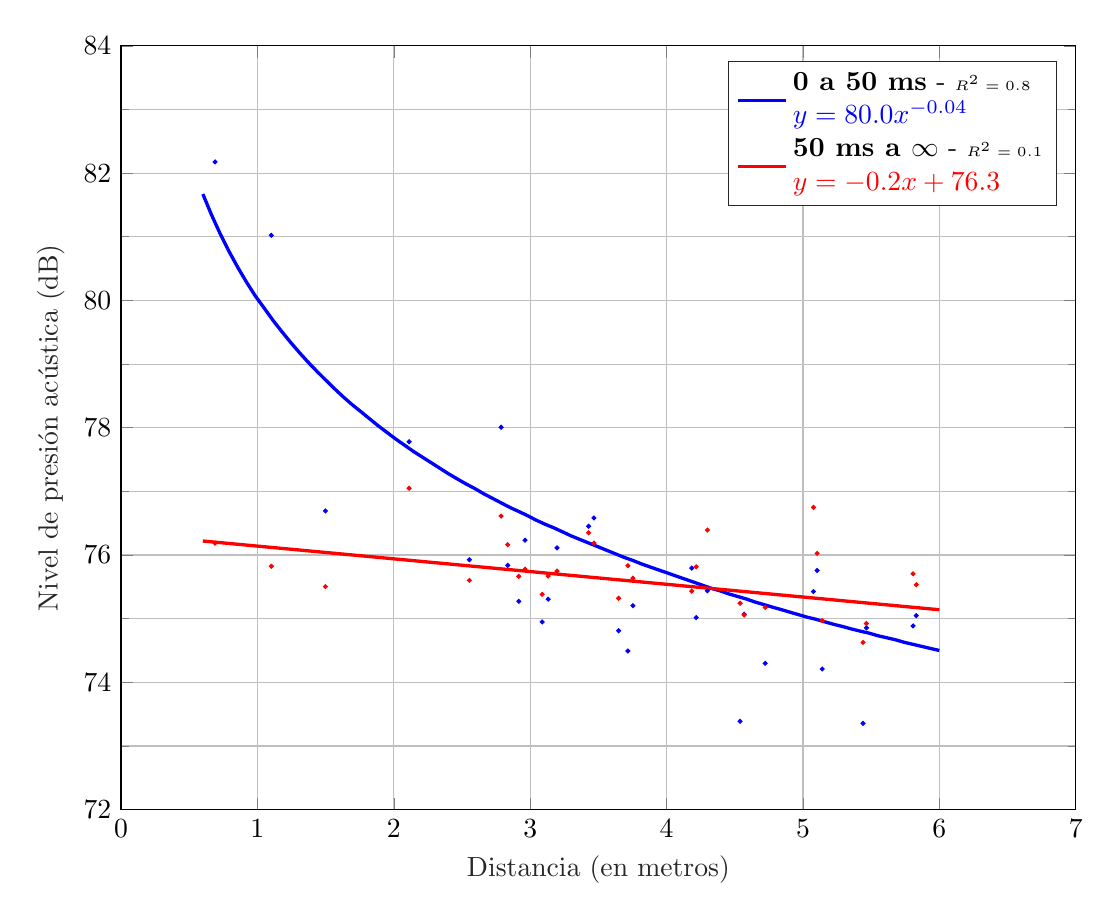
\begin{tikzpicture}

\begin{axis}[%
width=\textwidth,
height=0.8\textwidth,
at={(0\textwidth,0\textwidth)},
scale only axis,
xmin=0,
xmax=7,
xlabel style={font=\color{white!15!black}},
xlabel={Distancia (en metros)},
ymin=72,
ymax=84,
xmajorgrids,
xminorgrids,
ymajorgrids,
yminorgrids,
minor y tick num= 1,
ylabel style={font=\color{white!15!black}},
ylabel={Nivel de presión acústica (dB)},
axis background/.style={fill=white},
legend style={legend cell align=left, align=left, draw=white!15!black}
]
\addplot [color=blue, only marks,mark size=0.7pt, forget plot]
  table[row sep=crcr]{%
0.689492567037533	82.1760231834145\\
1.10208892563169	81.0225435793872\\
1.49833240637717	76.6929736552575\\
2.11248668634857	77.7797341548963\\
2.5540947515705	75.9268678204342\\
2.78664673039121	78.0078667294989\\
2.83511904511963	75.8379926821758\\
2.91626473421053	75.2733361947342\\
2.9626170862938	76.2332705870363\\
3.08787953132891	74.9482250490155\\
3.13169283295792	75.3064321486077\\
3.19677962956473	76.1127065991513\\
3.428206528201	76.4517777633818\\
3.46772259559498	76.5818812618574\\
3.64836949883095	74.8090226514553\\
3.71663826596024	74.4921848339607\\
3.75311870315875	75.2041666937952\\
4.18442349673165	75.7926859018596\\
4.21685902064559	75.0167269886588\\
4.29941856534113	75.4385466917373\\
4.53878838458019	73.3872229047654\\
4.56870878914383	75.0707133021758\\
4.72298634340605	74.2990289518437\\
5.07690850813761	75.4267529690394\\
5.10367514640186	75.757487280947\\
5.14125471067132	74.2096029808742\\
5.44027572830643	73.3546647587015\\
5.46526303118158	74.8548020040326\\
5.80710771382795	74.8859657158564\\
5.83052313261855	75.0478888373477\\
};

\addplot[color=blue,domain=0.6:6, samples=85,line width=1.2]{80.02*x^(-0.04)};
\addlegendentry{\textbf{0 a 50 ms} - \tiny{$R^2 = 0.8$}\\$\color{blue}y = 80.0·x^{-0.04}$}


\addplot [color=red, only marks,mark size=0.7pt, forget plot]
  table[row sep=crcr]{%
0.689492567037533	76.1860324366908\\
1.10208892563169	75.8228245224521\\
1.49833240637717	75.5036949938464\\
2.11248668634857	77.0497144256298\\
2.5540947515705	75.6014044921133\\
2.78664673039121	76.6112713817978\\
2.83511904511963	76.162080733805\\
2.91626473421053	75.6651404039956\\
2.9626170862938	75.7775619322898\\
3.08787953132891	75.3821777509942\\
3.13169283295792	75.6687522168879\\
3.19677962956473	75.7477124982068\\
3.428206528201	76.3485162347617\\
3.46772259559498	76.185858536935\\
3.64836949883095	75.3211330582598\\
3.71663826596024	75.8324897336812\\
3.75311870315875	75.6357978606202\\
4.18442349673165	75.4316552399674\\
4.21685902064559	75.8139630101425\\
4.29941856534113	76.3919969989648\\
4.53878838458019	75.2420141497027\\
4.56870878914383	75.0580538595667\\
4.72298634340605	75.1774090440704\\
5.07690850813761	76.7490410724972\\
5.10367514640186	76.0255133429585\\
5.14125471067132	74.9683820360272\\
5.44027572830643	74.6258521636235\\
5.46526303118158	74.9241893689036\\
5.80710771382795	75.7043411902589\\
5.83052313261855	75.5332426529618\\
};
\addplot[color=red,domain=0.6:6, samples=85,line width=1.2]{-0.2*x+76.34};
\addlegendentry{\textbf{50 ms a $\infty$} - \tiny{$R^2 = 0.1$}\\$\color{red}y = -0.2·x+76.3$}

\end{axis}
\end{tikzpicture}%%
    }
    \caption{Fuente en el centro}%
    \end{subfigure}
    \caption{Campos acústicos en el aula EP/0-26M con mobiliario. 30 puntos de medida}
    \label{graf:epsmob}%
\end{figure}
\FloatBarrier 

En el caso con mobiliario (figura \ref{graf:epsmob}), la distancia de cruce de campos con fuente en esquina es de 8.5 metros, con fuente en el centro es de 4.3 metros. Se han realizado un total de 30 medidas en diferentes puntos.

\begin{figure}[ht]
    \begin{subfigure}[b]{0.4\textwidth}
    	\centering%
         {\scalefont{0.8}%
    %%%%%%%%%%%%%%%%%%%%%%%%%%%%%%%%%%%%%%%%%%%%%%%%%%%%%%%%%%%%%%%%%%%%%%%%
% Escuela Politécnica Superior de la Universidad de Alicante
% Realizado por: Jose Manuel Requena Plens
% Contacto: info@jmrplens.com / Telegram:@jmrplens
%%%%%%%%%%%%%%%%%%%%%%%%%%%%%%%%%%%%%%%%%%%%%%%%%%%%%%%%%%%%%%%%%%%%%%%%

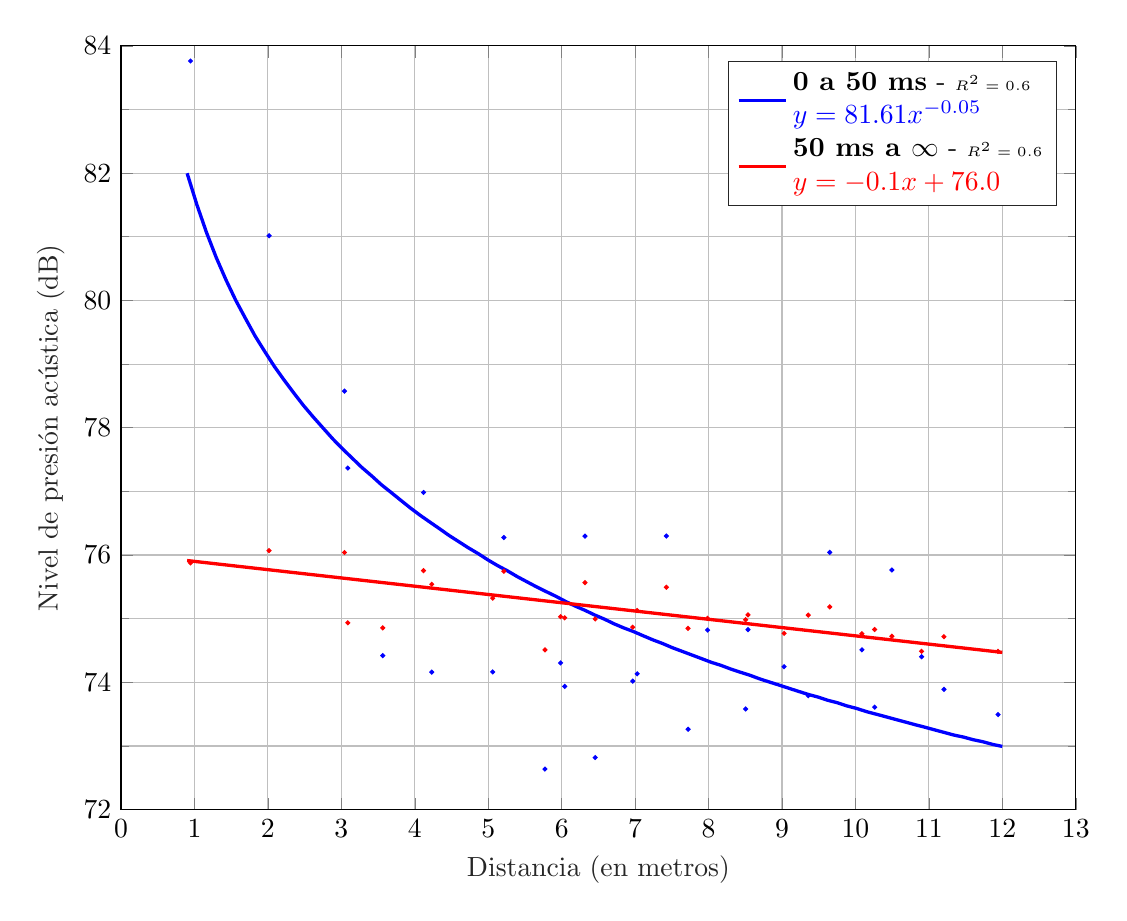
\begin{tikzpicture}

\begin{axis}[%
width=\textwidth,
height=0.8\textwidth,
at={(0\textwidth,0\textwidth)},
scale only axis,
xmin=0,
xmax=13,
xlabel style={font=\color{white!15!black}},
xlabel={Distancia (en metros)},
ymin=72,
ymax=84,
xmajorgrids,
xminorgrids,
ymajorgrids,
yminorgrids,
minor y tick num= 1,
ylabel style={font=\color{white!15!black}},
ylabel={Nivel de presión acústica (dB)},
axis background/.style={fill=white},
legend style={legend cell align=left, align=left, draw=white!15!black}
]
\addplot [color=blue, only marks,mark size=0.7pt, forget plot]
  table[row sep=crcr]{%
0.945832966226064	83.7613723273159\\
2.0155892438689	81.0162423459966\\
3.04292622322659	78.5741340871889\\
3.08781476128345	77.3661694070126\\
3.56407070636934	74.4195447651733\\
4.11885906532379	76.9825018479041\\
4.23076825174815	74.1614948370034\\
5.0601383380299	74.1635047432433\\
5.21338661524349	76.2742875281612\\
5.7725297747175	72.6376750158334\\
5.98493107729738	74.3045302985103\\
6.04070360140274	73.9359821507463\\
6.31685048105462	76.2962616688626\\
6.45653932071973	72.8184525162864\\
6.96725196903341	74.0197233913669\\
7.02797979507625	74.1332978831264\\
7.42526767194288	76.2979528676753\\
7.72055049850721	73.2624003422856\\
7.98590007450632	74.8209368605219\\
8.5047104595042	73.5815675022983\\
8.53670896774629	74.8278098704551\\
9.02858792946051	74.2461859060413\\
9.35746226281464	73.7897862980008\\
9.65012953280939	76.0413437836555\\
10.0878639959111	74.5098029500084\\
10.2617201287114	73.6092755871979\\
10.4960706933595	75.7646635864789\\
10.8998853204976	74.4019326738631\\
11.2050211958747	73.8894451766927\\
11.9413148354777	73.4937384336641\\
};
\addplot[color=blue,domain=0.9:12, samples=85,line width=1.2]{81.61*x^(-0.045)};
\addlegendentry{\textbf{0 a 50 ms} - \tiny{$R^2 = 0.6$}\\$\color{blue}y = 81.61·x^{-0.05}$}

\addplot [color=red, only marks,mark size=0.7pt, forget plot]
  table[row sep=crcr]{%
0.945832966226064	75.8756831712236\\
2.0155892438689	76.0688117402114\\
3.04292622322659	76.0395356654983\\
3.08781476128345	74.9352478473615\\
3.56407070636934	74.8553844312649\\
4.11885906532379	75.7543937944735\\
4.23076825174815	75.540482339615\\
5.0601383380299	75.3223520645197\\
5.21338661524349	75.7450970961607\\
5.7725297747175	74.5101521130851\\
5.98493107729738	75.0309510163013\\
6.04070360140274	75.0132759751214\\
6.31685048105462	75.5655547954218\\
6.45653932071973	74.9956410748914\\
6.96725196903341	74.8655502346388\\
7.02797979507625	75.1283568472655\\
7.42526767194288	75.4940077965527\\
7.72055049850721	74.8471381044347\\
7.98590007450632	75.004616004375\\
8.5047104595042	74.9841736554508\\
8.53670896774629	75.0586998621683\\
9.02858792946051	74.7687602281066\\
9.35746226281464	75.0566535033458\\
9.65012953280939	75.1842952487827\\
10.0878639959111	74.7630381678478\\
10.2617201287114	74.8297960943133\\
10.4960706933595	74.7247830880759\\
10.8998853204976	74.4871393636727\\
11.2050211958747	74.7165933582166\\
11.9413148354777	74.4864585207557\\
};
\addplot[color=red,domain=0.9:12, samples=85,line width=1.2]{-0.13*x+76.03};
\addlegendentry{\textbf{50 ms a $\infty$} - \tiny{$R^2 = 0.6$}\\$\color{red}y = -0.1·x+76.0$}

\end{axis}
\end{tikzpicture}%%
    }
    \caption{Fuente en la esquina}%
    \end{subfigure}%
    \hspace{1.9cm}%
    \begin{subfigure}[b]{0.4\textwidth}%
    	\centering%
        {\scalefont{0.8}%
    %%%%%%%%%%%%%%%%%%%%%%%%%%%%%%%%%%%%%%%%%%%%%%%%%%%%%%%%%%%%%%%%%%%%%%%%
% Escuela Politécnica Superior de la Universidad de Alicante
% Realizado por: Jose Manuel Requena Plens
% Contacto: info@jmrplens.com / Telegram:@jmrplens
%%%%%%%%%%%%%%%%%%%%%%%%%%%%%%%%%%%%%%%%%%%%%%%%%%%%%%%%%%%%%%%%%%%%%%%%


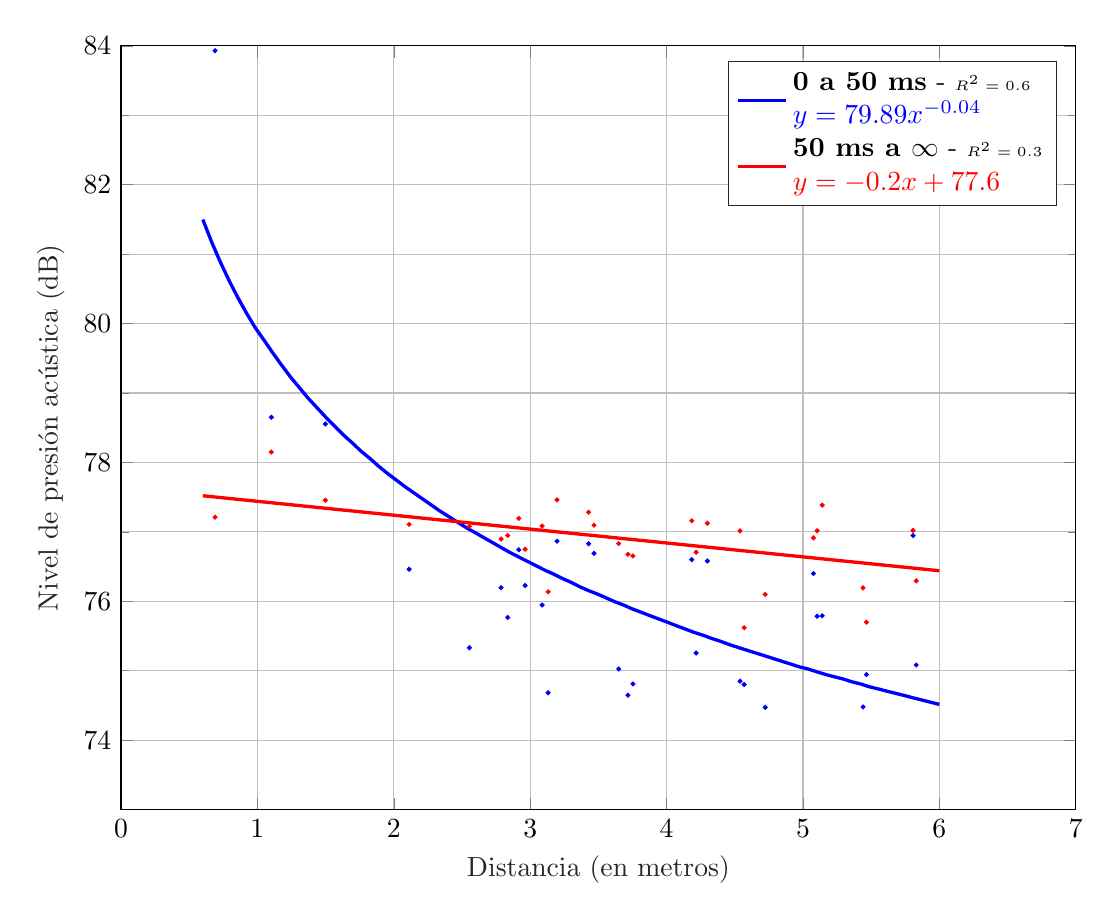
\begin{tikzpicture}

\begin{axis}[%
width=\textwidth,
height=0.8\textwidth,
at={(0\textwidth,0\textwidth)},
scale only axis,
xmin=0,
xmax=7,
xlabel style={font=\color{white!15!black}},
xlabel={Distancia (en metros)},
ymin=73,
ymax=84,
xmajorgrids,
xminorgrids,
ymajorgrids,
yminorgrids,
minor y tick num= 1,
ylabel style={font=\color{white!15!black}},
ylabel={Nivel de presión acústica (dB)},
axis background/.style={fill=white},
legend style={legend cell align=left, align=left, draw=white!15!black}
]
\addplot [color=blue, only marks,mark size=0.7pt, forget plot]
  table[row sep=crcr]{%
0.689492567037533	83.9298147556326\\
1.10208892563169	78.6508839586394\\
1.49833240637717	78.5537850719206\\
2.11248668634857	76.4616696030503\\
2.5540947515705	75.3307670198302\\
2.78664673039121	76.1965578400623\\
2.83511904511963	75.7676896799252\\
2.91626473421053	76.7421442885895\\
2.9626170862938	76.2279520874836\\
3.08787953132891	75.946910653961\\
3.13169283295792	74.682472152864\\
3.19677962956473	76.8654178100693\\
3.428206528201	76.8298033992244\\
3.46772259559498	76.6907385817452\\
3.64836949883095	75.0265374586113\\
3.71663826596024	74.6483005887243\\
3.75311870315875	74.8106601341298\\
4.18442349673165	76.6001904524153\\
4.21685902064559	75.2548274781649\\
4.29941856534113	76.5801826216203\\
4.53878838458019	74.8502307135703\\
4.56870878914383	74.8015849348429\\
4.72298634340605	74.4730406896843\\
5.07690850813761	76.4002346735743\\
5.10367514640186	75.7856409590404\\
5.14125471067132	75.7915936696579\\
5.44027572830643	74.4783975819506\\
5.46526303118158	74.9451316191164\\
5.80710771382795	76.9464967378256\\
5.83052313261855	75.0825990403115\\
};

\addplot[color=blue,domain=0.6:6, samples=85,line width=1.2]{79.89*x^(-0.039)};
\addlegendentry{\textbf{0 a 50 ms} - \tiny{$R^2 = 0.6$}\\$\color{blue}y = 79.89·x^{-0.04}$}


\addplot [color=red, only marks,mark size=0.7pt, forget plot]
  table[row sep=crcr]{%
0.689492567037533	77.2116251901105\\
1.10208892563169	78.1487656108054\\
1.49833240637717	77.4554982654753\\
2.11248668634857	77.1079070401778\\
2.5540947515705	77.0793479410879\\
2.78664673039121	76.8967227680043\\
2.83511904511963	76.9480634611297\\
2.91626473421053	77.1929999186771\\
2.9626170862938	76.7497664684574\\
3.08787953132891	77.0846862461668\\
3.13169283295792	76.136335003754\\
3.19677962956473	77.4614429688778\\
3.428206528201	77.2839536491472\\
3.46772259559498	77.0950077390861\\
3.64836949883095	76.8304860918788\\
3.71663826596024	76.6765715504004\\
3.75311870315875	76.6532524648088\\
4.18442349673165	77.1602815406925\\
4.21685902064559	76.7070937423991\\
4.29941856534113	77.1239304562105\\
4.53878838458019	77.0144084058593\\
4.56870878914383	75.6204899031107\\
4.72298634340605	76.0991888395833\\
5.07690850813761	76.9133557074926\\
5.10367514640186	77.0156266301233\\
5.14125471067132	77.3844643413919\\
5.44027572830643	76.1925753967431\\
5.46526303118158	75.6991412964459\\
5.80710771382795	77.0214783572162\\
5.83052313261855	76.2932567913482\\
};
\addplot[color=red,domain=0.6:6, samples=85,line width=1.2]{-0.2*x+77.64};
\addlegendentry{\textbf{50 ms a $\infty$} - \tiny{$R^2 = 0.3$}\\$\color{red}y = -0.2·x+77.6$}

\end{axis}
\end{tikzpicture}%%
    }
    \caption{Fuente en el centro}%
    \end{subfigure}
    \caption{Campos acústicos en el aula EP/0-26M sin mobiliario. 30 puntos de medida}
    \label{graf:epsnomob}%
\end{figure}
\FloatBarrier 

En el caso sin mobiliario (figura \ref{graf:epsnomob}), la distancia de cruce de campos con fuente en esquina es de 6.1 metros, con fuente en el centro es de 2.5 metros. Se han realizado un total de 30 medidas en diferentes puntos. 
\\
\par
Como se ha podido observar en las figuras \ref{graf:epsmob} y \ref{graf:epsnomob} existe una alta variabilidad en los valores respecto a la distancia dando un ajuste de curva muy bajo en general. Esta variabilidad puede ser producida por:
\begin{itemize}
\itemsep0em
  \item El efecto de focalizaciones debido a la reflexiones de las ventanas (ocupan un 33\% de una de las paredes). 
  \item Por la aparición de modos propios. La frecuencia límite (ecuación \ref{ecu:schroeder}) es de  154 Hz para el recinto con mobiliario y de 162 sin él, una pequeña parte del espectro total (125 Hz a 8 kHz) por tanto no debería afectar al nivel de presión acústica global. 
  
  	  Aún así se debería analizar espacialmente pero no es posible obtener resultados fiables debido a que la distancia entre puntos de medida en el eje X es de 1 metro, en el eje Y de 3 metros aproximadamente y en el eje Z tan sólo hay un punto a 1.2 metros de altura, para analizar la existencia de modos se necesitan al menos una distancia entre puntos de $\nicefrac{\lambda}{4}$. Con la distancia de puntos actual sólo se puede analizar hasta la frecuencia de 86 Hz en el eje X y hasta 28 Hz en el eje Y, en el eje Z al tener sólo un punto de medida no se puede analizar este comportamiento, por lo que si existe una respuesta modal no es posible confirmarla con los datos que se han obtenido actualmente, sería necesario aumentar los puntos de medida.
\end{itemize}
Se puede observar claramente en los mapas de nivel de presión acústica de los campos perjudiciales (\ref{graf:mapaepsperjudicialcon} y \ref{graf:mapaepsperjudicialsin}) la razón de la alta variabilidad de los niveles respecto a la distancia.

%%%%%
%%%%% MAPAS EPS
%%%%%

\begin{figure}[H]
    \centering%
        {\scalefont{0.8}%
    %%%%%%%%%%%%%%%%%%%%%%%%%%%%%%%%%%%%%%%%%%%%%%%%%%%%%%%%%%%%%%%%%%%%%%%%
% Escuela Politécnica Superior de la Universidad de Alicante
% Realizado por: Jose Manuel Requena Plens
% Contacto: info@jmrplens.com / Telegram:@jmrplens
%%%%%%%%%%%%%%%%%%%%%%%%%%%%%%%%%%%%%%%%%%%%%%%%%%%%%%%%%%%%%%%%%%%%%%%%

\begin{tikzpicture}

\begin{groupplot}[
      group style = {
        group size = 2 by 1,
        horizontal sep = 2cm,
      },
      view = {0}{90},
      colormap name=jet,
      ]
      
  % GRAFICA 1
  \nextgroupplot[
  	width=0.45\textwidth,
  	view={0}{90},
	xlabel style={font=\color{white!15!black}},
	xlabel={Lx (m)},
	ylabel style={font=\color{white!15!black}},
	ylabel={Ly (m)},
	axis equal image=true,
	point meta min=72,
	point meta max=84,
%          colorbar horizontal,
%          colorbar style = {
%          	xlabel={Nivel de presión acústica (dB)},
%            at={(rel axis cs: 1.1,-0.3)},
%            anchor=south,
%            height=3mm,
%            axis line style={draw=none}
%          },
	colorbar,
	colorbar style = {
		ylabel={SPL (dB)},
	at={(rel axis cs: 1.11,1)},
	ylabel style={font=\normalfont,at={(rel axis cs: -2.8,0.5)}},
	%anchor=south,
	width=2mm,
	ytick distance=3,
	axis line style={draw=none}
	},
	]

	\addplot3 [
    	surf,
    	shader=interp,
    	mesh/cols=39,mesh/ordering=y varies,
	]
    	table {archivos/graficastikz/EPSLlenoEsquinaUtilMalla.dat};
    	
    	
    % Imprime la fuente
\addplot[only marks,mark=*,white,mark size=3pt,mark options={fill=black}]
    	coordinates {
    	(0.6,6.5)
    	};	
    	
    % Imprime los receptores
\addplot[only marks,mark=triangle*,white, mark size=2pt, mark options={fill=blue}]
    	coordinates {
    	(11.05,6.25)
		(10.20,6.25)
		(9.08,6.25)
		(7.96,6.25)
		(6.84,6.25)
		(5.72,6.25)
		(4.60,6.25)
		(3.48,6.25)
		(2.36,6.25)
		(1.24,6.25)
		(11.05,3.55)
		(10.20,3.55)
		(9.08,3.55)
		(7.96,3.55)
		(6.84,3.55)
		(5.72,3.55)
		(4.60,3.55)
		(3.48,3.55)
		(2.36,3.55)
		(1.24,3.55)
		(11.05,0.80)
		(10.20,0.80)
		(9.08,0.80)
		(7.96,0.80)
		(6.84,0.80)
		(5.72,0.80)
		(4.60,0.80)
		(3.48,0.80)
		(2.36,0.80)
		(1.24,0.80)
		};	
		
	% GRAFICA 2
  \nextgroupplot[
  	width=0.45\textwidth,
  	view={0}{90},
	xlabel style={font=\color{white!15!black}},
	xlabel={Lx (m)},
	ylabel style={font=\color{white!15!black}},
	ylabel={Ly (m)},
	axis equal image=true,
	point meta min=72,
	point meta max=84,
	yticklabel pos=right,
	]
	
	\addplot3 [
    	surf,
    	shader=interp,
    	mesh/cols=39,mesh/ordering=y varies,
	]
    	table {archivos/graficastikz/EPSLlenoCentroUtilMalla.dat};
    	
    	
    % Imprime la fuente
    \addplot[only marks,mark=*,white,mark size=3pt,mark options={fill=black}]
    	coordinates {
    	(5.95,3.55)
    	};	
    	
    % Imprime los receptores
    \addplot[only marks,mark=triangle*,white, mark size=2pt, mark options={fill=blue}]
    	coordinates {
    	(11.05,6.25)
		(10.20,6.25)
		(9.08,6.25)
		(7.96,6.25)
		(6.84,6.25)
		(5.72,6.25)
		(4.60,6.25)
		(3.48,6.25)
		(2.36,6.25)
		(1.24,6.25)
		(11.05,3.55)
		(10.20,3.55)
		(9.08,3.55)
		(7.96,3.55)
		(6.84,3.55)
		(5.72,3.55)
		(4.60,3.55)
		(3.48,3.55)
		(2.36,3.55)
		(1.24,3.55)
		(11.05,0.80)
		(10.20,0.80)
		(9.08,0.80)
		(7.96,0.80)
		(6.84,0.80)
		(5.72,0.80)
		(4.60,0.80)
		(3.48,0.80)
		(2.36,0.80)
		(1.24,0.80)
		};	
\end{groupplot}

\end{tikzpicture}%%
    }
    \caption{Campos útiles (0 a 50 ms) para ambas posiciones de fuente en el aula EP/0-26M con mobiliario. Las fuentes (círculos) y los 30 puntos de medida (triángulos)}
    \label{graf:mapaepsutilcon}%
\end{figure} 

\begin{figure}[H]
    \centering%
        {\scalefont{0.8}%
    %%%%%%%%%%%%%%%%%%%%%%%%%%%%%%%%%%%%%%%%%%%%%%%%%%%%%%%%%%%%%%%%%%%%%%%%
% Escuela Politécnica Superior de la Universidad de Alicante
% Realizado por: Jose Manuel Requena Plens
% Contacto: info@jmrplens.com / Telegram:@jmrplens
%%%%%%%%%%%%%%%%%%%%%%%%%%%%%%%%%%%%%%%%%%%%%%%%%%%%%%%%%%%%%%%%%%%%%%%%

\begin{tikzpicture}

\begin{groupplot}[
      group style = {
        group size = 2 by 1,
        horizontal sep = 2cm,
      },
      view = {0}{90},
      colormap name=jet,
      ]
      
  % GRAFICA 1
  \nextgroupplot[
  	width=0.45\textwidth,
  	view={0}{90},
	xlabel style={font=\color{white!15!black}},
	xlabel={Lx (m)},
	ylabel style={font=\color{white!15!black}},
	ylabel={Ly (m)},
	axis equal image=true,
	point meta min=72,
	point meta max=84,
%          colorbar horizontal,
%          colorbar style = {
%          	xlabel={Nivel de presión acústica (dB)},
%            at={(rel axis cs: 1.1,-0.3)},
%            anchor=south,
%            height=3mm,
%            axis line style={draw=none}
%          },
	colorbar,
	colorbar style = {
		ylabel={SPL (dB)},
	at={(rel axis cs: 1.11,1)},
	ylabel style={font=\normalfont,at={(rel axis cs: -2.8,0.5)}},
	%anchor=south,
	width=2mm,
	ytick distance=3,
	axis line style={draw=none}
	},
	]

	\addplot3 [
    	surf,
    	shader=interp,
    	mesh/cols=39,mesh/ordering=y varies,
	]
    	table {archivos/graficastikz/EPSVacioEsquinaUtilMalla.dat};
    	
    	
    % Imprime la fuente
\addplot[only marks,mark=*,white,mark size=3pt,mark options={fill=black}]
    	coordinates {
    	(0.6,6.5)
    	};	
    	
    % Imprime los receptores
\addplot[only marks,mark=triangle*,white, mark size=2pt, mark options={fill=blue}]
    	coordinates {
    	(11.05,6.25)
		(10.20,6.25)
		(9.08,6.25)
		(7.96,6.25)
		(6.84,6.25)
		(5.72,6.25)
		(4.60,6.25)
		(3.48,6.25)
		(2.36,6.25)
		(1.24,6.25)
		(11.05,3.55)
		(10.20,3.55)
		(9.08,3.55)
		(7.96,3.55)
		(6.84,3.55)
		(5.72,3.55)
		(4.60,3.55)
		(3.48,3.55)
		(2.36,3.55)
		(1.24,3.55)
		(11.05,0.80)
		(10.20,0.80)
		(9.08,0.80)
		(7.96,0.80)
		(6.84,0.80)
		(5.72,0.80)
		(4.60,0.80)
		(3.48,0.80)
		(2.36,0.80)
		(1.24,0.80)
		};	
		
	% GRAFICA 2
  \nextgroupplot[
  	width=0.45\textwidth,
  	view={0}{90},
	xlabel style={font=\color{white!15!black}},
	xlabel={Lx (m)},
	ylabel style={font=\color{white!15!black}},
	ylabel={Ly (m)},
	axis equal image=true,
	point meta min=72,
	point meta max=84,
	yticklabel pos=right,
	]
	
	\addplot3 [
    	surf,
    	shader=interp,
    	mesh/cols=39,mesh/ordering=y varies,
	]
    	table {archivos/graficastikz/EPSVacioCentroUtilMalla.dat};
    	
    	
    % Imprime la fuente
\addplot[only marks,mark=*,white,mark size=3pt,mark options={fill=black}]
    	coordinates {
    	(5.95,3.55)
    	};	
    	
    % Imprime los receptores
\addplot[only marks,mark=triangle*,white, mark size=2pt, mark options={fill=blue}]
    	coordinates {
    	(11.05,6.25)
		(10.20,6.25)
		(9.08,6.25)
		(7.96,6.25)
		(6.84,6.25)
		(5.72,6.25)
		(4.60,6.25)
		(3.48,6.25)
		(2.36,6.25)
		(1.24,6.25)
		(11.05,3.55)
		(10.20,3.55)
		(9.08,3.55)
		(7.96,3.55)
		(6.84,3.55)
		(5.72,3.55)
		(4.60,3.55)
		(3.48,3.55)
		(2.36,3.55)
		(1.24,3.55)
		(11.05,0.80)
		(10.20,0.80)
		(9.08,0.80)
		(7.96,0.80)
		(6.84,0.80)
		(5.72,0.80)
		(4.60,0.80)
		(3.48,0.80)
		(2.36,0.80)
		(1.24,0.80)
		};	
\end{groupplot}

\end{tikzpicture}%%
    }
    \caption{Campos útiles (0 a 50 ms) para ambas posiciones de fuente en el aula EP/0-26M sin mobiliario. Las fuentes (círculos) y los 30 puntos de medida (triángulos)}
    \label{graf:mapaepsutilsin}%
\end{figure}

En las figuras \ref{graf:mapaepsutilcon} y \ref{graf:mapaepsutilsin} se muestran los mapas del campo útil con y sin mobiliario, el comportamiento es muy similar en ambos teniendo un mayor nivel en ciertas zonas cuando se retira el mobiliario. En los mapas se producen algunos artefactos en la zona de extrapolación (abarca desde los puntos de medida hasta los límites del recinto), sobretodo es notable en la esquina superior izquierda del aula sin mobiliario y fuente en el centro.
\\
\par 
En los mapas de campo perjudicial (figuras \ref{graf:mapaepsperjudicialcon} y \ref{graf:mapaepsperjudicialsin}) es donde se aprecia la razón de los valores tan bajos en el ajuste de las curvas anteriores. En todos los mapas de campo perjudicial, que contienen la mayoría de la energía acústica en términos temporales, se obtienen niveles muy variantes respecto a la distancia a la fuente. El comportamiento es muy similar a un campo estacionario en un tubo cerrado, comportamiento estudiado inicialmente en \cite{Kundt1866} y \cite{Kundt1868}, donde la energía acústica se mantiene estacionaria a lo largo de éste. Con la fuente en la esquina este efecto es menor que con la fuente en el centro debido a que, si la fuente no está equidistanciada de los planos de las paredes, no puede formar campos estacionarios o focalizaciones tan acusadas como se producirían con la fuente posicionada en el centro.

\begin{figure}[H]
    \centering%
        {\scalefont{0.8}%
    %%%%%%%%%%%%%%%%%%%%%%%%%%%%%%%%%%%%%%%%%%%%%%%%%%%%%%%%%%%%%%%%%%%%%%%%
% Escuela Politécnica Superior de la Universidad de Alicante
% Realizado por: Jose Manuel Requena Plens
% Contacto: info@jmrplens.com / Telegram:@jmrplens
%%%%%%%%%%%%%%%%%%%%%%%%%%%%%%%%%%%%%%%%%%%%%%%%%%%%%%%%%%%%%%%%%%%%%%%%

\begin{tikzpicture}

\begin{groupplot}[
      group style = {
        group size = 2 by 1,
        horizontal sep = 2cm,
      },
      view = {0}{90},
      colormap name=jet,
      ]
      
  % GRAFICA 1
  \nextgroupplot[
  	width=0.45\textwidth,
  	view={0}{90},
	xlabel style={font=\color{white!15!black}},
	xlabel={Lx (m)},
	ylabel style={font=\color{white!15!black}},
	ylabel={Ly (m)},
	axis equal image=true,
	point meta min=72,
	point meta max=78,
%          colorbar horizontal,
%          colorbar style = {
%          	xlabel={Nivel de presión acústica (dB)},
%            at={(rel axis cs: 1.1,-0.3)},
%            anchor=south,
%            height=3mm,
%            axis line style={draw=none}
%          },
	colorbar,
	colorbar style = {
		ylabel={SPL (dB)},
	at={(rel axis cs: 1.11,1)},
	ylabel style={font=\normalfont,at={(rel axis cs: -2.8,0.5)}},
	%anchor=south,
	width=2mm,
	axis line style={draw=none}
	},
	]

	\addplot3 [
    	surf,
    	shader=interp,
    	mesh/cols=39,mesh/ordering=y varies,
	]
    	table {archivos/graficastikz/EPSLlenoEsquinaPerjudicialMalla.dat};
    	
    	
    % Imprime la fuente
\addplot[only marks,mark=*,white,mark size=3pt,mark options={fill=black}]
    	coordinates {
    	(0.6,6.5)
    	};	
    	
    % Imprime los receptores
\addplot[only marks,mark=triangle*,white, mark size=2pt, mark options={fill=blue}]
    	coordinates {
    	(11.05,6.25)
		(10.20,6.25)
		(9.08,6.25)
		(7.96,6.25)
		(6.84,6.25)
		(5.72,6.25)
		(4.60,6.25)
		(3.48,6.25)
		(2.36,6.25)
		(1.24,6.25)
		(11.05,3.55)
		(10.20,3.55)
		(9.08,3.55)
		(7.96,3.55)
		(6.84,3.55)
		(5.72,3.55)
		(4.60,3.55)
		(3.48,3.55)
		(2.36,3.55)
		(1.24,3.55)
		(11.05,0.80)
		(10.20,0.80)
		(9.08,0.80)
		(7.96,0.80)
		(6.84,0.80)
		(5.72,0.80)
		(4.60,0.80)
		(3.48,0.80)
		(2.36,0.80)
		(1.24,0.80)
		};	
		
	% GRAFICA 2
  \nextgroupplot[
  	width=0.45\textwidth,
  	view={0}{90},
	xlabel style={font=\color{white!15!black}},
	xlabel={Lx (m)},
	ylabel style={font=\color{white!15!black}},
	ylabel={Ly (m)},
	axis equal image=true,
	point meta min=72,
	point meta max=78,
	yticklabel pos=right,
	]
	
	\addplot3 [
    	surf,
    	shader=interp,
    	mesh/cols=39,mesh/ordering=y varies,
	]
    	table {archivos/graficastikz/EPSLlenoCentroPerjudicialMalla.dat};
    	
    	
    % Imprime la fuente
\addplot[only marks,mark=*,white,mark size=3pt,mark options={fill=black}]
    	coordinates {
    	(5.95,3.55)
    	};	
    	
    % Imprime los receptores
\addplot[only marks,mark=triangle*,white, mark size=2pt, mark options={fill=blue}]
    	coordinates {
    	(11.05,6.25)
		(10.20,6.25)
		(9.08,6.25)
		(7.96,6.25)
		(6.84,6.25)
		(5.72,6.25)
		(4.60,6.25)
		(3.48,6.25)
		(2.36,6.25)
		(1.24,6.25)
		(11.05,3.55)
		(10.20,3.55)
		(9.08,3.55)
		(7.96,3.55)
		(6.84,3.55)
		(5.72,3.55)
		(4.60,3.55)
		(3.48,3.55)
		(2.36,3.55)
		(1.24,3.55)
		(11.05,0.80)
		(10.20,0.80)
		(9.08,0.80)
		(7.96,0.80)
		(6.84,0.80)
		(5.72,0.80)
		(4.60,0.80)
		(3.48,0.80)
		(2.36,0.80)
		(1.24,0.80)
		};	
\end{groupplot}

\end{tikzpicture}%%
    }
    \caption{Campos perjudiciales (50 ms a $\infty$) para ambas posiciones de fuente en el aula EP/0-26M con mobiliario. Las fuentes (círculos) y los 30 puntos de medida (triángulos)}
    \label{graf:mapaepsperjudicialcon}%
    \vspace{-0.4cm}%
\end{figure}


\begin{figure}[H]
    \centering%
        {\scalefont{0.8}%
    %%%%%%%%%%%%%%%%%%%%%%%%%%%%%%%%%%%%%%%%%%%%%%%%%%%%%%%%%%%%%%%%%%%%%%%%
% Escuela Politécnica Superior de la Universidad de Alicante
% Realizado por: Jose Manuel Requena Plens
% Contacto: info@jmrplens.com / Telegram:@jmrplens
%%%%%%%%%%%%%%%%%%%%%%%%%%%%%%%%%%%%%%%%%%%%%%%%%%%%%%%%%%%%%%%%%%%%%%%%

\begin{tikzpicture}

\begin{groupplot}[
      group style = {
        group size = 2 by 1,
        horizontal sep = 2cm,
      },
      view = {0}{90},
      colormap name=jet,
      ]
      
  % GRAFICA 1
  \nextgroupplot[
  	width=0.45\textwidth,
  	view={0}{90},
	xlabel style={font=\color{white!15!black}},
	xlabel={Lx (m)},
	ylabel style={font=\color{white!15!black}},
	ylabel={Ly (m)},
	axis equal image=true,
	point meta min=74,
	point meta max=78,
%          colorbar horizontal,
%          colorbar style = {
%          	xlabel={Nivel de presión acústica (dB)},
%            at={(rel axis cs: 1.1,-0.3)},
%            anchor=south,
%            height=3mm,
%            axis line style={draw=none}
%          },
	colorbar,
	colorbar style = {
		ylabel={SPL (dB)},
	at={(rel axis cs: 1.11,1)},
	ylabel style={font=\normalfont,at={(rel axis cs: -2.8,0.5)}},
	%anchor=south,
	width=2mm,
	axis line style={draw=none}
	},
	]

	\addplot3 [
    	surf,
    	shader=interp,
    	mesh/cols=39,mesh/ordering=y varies,
	]
    	table {archivos/graficastikz/EPSVacioEsquinaPerjudicialMalla.dat};
    	
    	
    % Imprime la fuente
    \addplot[only marks,mark=*,black,mark size=3pt]
    	coordinates {
    	(0.6,6.5)
    	};	
    	
    % Imprime los receptores
\addplot[only marks,mark=triangle*,white, mark size=2pt, mark options={fill=blue}]
    	coordinates {
    	(11.05,6.25)
		(10.20,6.25)
		(9.08,6.25)
		(7.96,6.25)
		(6.84,6.25)
		(5.72,6.25)
		(4.60,6.25)
		(3.48,6.25)
		(2.36,6.25)
		(1.24,6.25)
		(11.05,3.55)
		(10.20,3.55)
		(9.08,3.55)
		(7.96,3.55)
		(6.84,3.55)
		(5.72,3.55)
		(4.60,3.55)
		(3.48,3.55)
		(2.36,3.55)
		(1.24,3.55)
		(11.05,0.80)
		(10.20,0.80)
		(9.08,0.80)
		(7.96,0.80)
		(6.84,0.80)
		(5.72,0.80)
		(4.60,0.80)
		(3.48,0.80)
		(2.36,0.80)
		(1.24,0.80)
		};	
		
	% GRAFICA 2
  \nextgroupplot[
  	width=0.45\textwidth,
  	view={0}{90},
	xlabel style={font=\color{white!15!black}},
	xlabel={Lx (m)},
	ylabel style={font=\color{white!15!black}},
	ylabel={Ly (m)},
	axis equal image=true,
	point meta min=74,
	point meta max=78,
	yticklabel pos=right,
	]
	
	\addplot3 [
    	surf,
    	shader=interp,
    	mesh/cols=39,mesh/ordering=y varies,
	]
    	table {archivos/graficastikz/EPSVacioCentroPerjudicialMalla.dat};
    	
    	
    % Imprime la fuente
\addplot[only marks,mark=*,white,mark size=3pt,mark options={fill=black}]
    	coordinates {
    	(5.95,3.55)
    	};	
    	
    % Imprime los receptores
\addplot[only marks,mark=triangle*,white, mark size=2pt, mark options={fill=blue}]
    	coordinates {
    	(11.05,6.25)
		(10.20,6.25)
		(9.08,6.25)
		(7.96,6.25)
		(6.84,6.25)
		(5.72,6.25)
		(4.60,6.25)
		(3.48,6.25)
		(2.36,6.25)
		(1.24,6.25)
		(11.05,3.55)
		(10.20,3.55)
		(9.08,3.55)
		(7.96,3.55)
		(6.84,3.55)
		(5.72,3.55)
		(4.60,3.55)
		(3.48,3.55)
		(2.36,3.55)
		(1.24,3.55)
		(11.05,0.80)
		(10.20,0.80)
		(9.08,0.80)
		(7.96,0.80)
		(6.84,0.80)
		(5.72,0.80)
		(4.60,0.80)
		(3.48,0.80)
		(2.36,0.80)
		(1.24,0.80)
		};	
\end{groupplot}

\end{tikzpicture}%%
    }
    \caption{Campos perjudiciales (50 ms a $\infty$) para ambas posiciones de fuente en el aula EP/0-26M sin mobiliario. Las fuentes (círculos) y los 30 puntos de medida (triángulos)}
    \label{graf:mapaepsperjudicialsin}%
\end{figure}

Se ha analizado por bandas de octava este comportamiento intentando poder confirmar las causas por las que se está produciendo la alta variabilidad del nivel de presión acústica y no se puede confirmar a ciencia cierta debido a lo comentado anteriormente. En la figura \ref{graf:mapaepsperjudicial125} se puede observar que en diferentes bandas de frecuencias el comportamiento es el mismo que con el nivel global, aparecen máximos y mínimos a una distancia media aproximada entre máximos de 2 metros en todas las bandas, que se podría concluir que es debido a posibles focalizaciones del sonido pero sin una mayor resolución de los puntos de medida es imposible confirmarlo.

Sería necesario volver a realizar mediciones en el aula EP/0-26M aumentando los puntos de medida, al menos en algunas zonas realizar medidas cada 0.17 metros con tres mallados de 4x4 puntos en los planos XY, XZ y YZ para obtener información fiable hasta los 500 Hz y comprobar si se mantiene el comportamiento obtenido en las medidas anteriores. Una vez realizado si la información no es concluyente se debe reducir la distancia entre puntos hasta los 0.02 metros correspondientes a $\nicefrac{\lambda}{4}$ de la frecuencia de 4 kHz y confirmar finalmente el comportamiento de los campos acústicos en el interior del recinto.

\begin{figure}[ht]
    \centering%
        {\scalefont{0.8}%
    %%%%%%%%%%%%%%%%%%%%%%%%%%%%%%%%%%%%%%%%%%%%%%%%%%%%%%%%%%%%%%%%%%%%%%%%
% Escuela Politécnica Superior de la Universidad de Alicante
% Realizado por: Jose Manuel Requena Plens
% Contacto: info@jmrplens.com / Telegram:@jmrplens
%%%%%%%%%%%%%%%%%%%%%%%%%%%%%%%%%%%%%%%%%%%%%%%%%%%%%%%%%%%%%%%%%%%%%%%%

\begin{tikzpicture}

\begin{groupplot}[
      group style = {
        group size = 2 by 2,
        vertical sep = 2.5cm,
        horizontal sep = 1cm,
      },
      view = {0}{90},
      width=0.45\textwidth,
      colormap name=jet,
      xtick distance=2,
      ytick distance=2,
      ]
      
  % GRAFICA 1
  \nextgroupplot[
  	view={0}{90},
  	title={\textbf{125 Hz}},
	xlabel style={font=\color{white!15!black}},
	xlabel={Lx (m)},
	ylabel style={font=\color{white!15!black}},
	ylabel={Ly (m)},
	point meta min=53,
	point meta max=66,
	axis equal image=true,
	colorbar horizontal,
	colorbar style = {
		xlabel={Nivel de presión acústica (dB)},
		xlabel style={font=\tiny,at={(rel axis cs: 0.5,-1.1)}},
		tick label style={font=\tiny}, 
		xtick distance=3,
		at={(rel axis cs: 0.5,-0.25)},
		anchor=south,
		height=2mm,
		axis line style={draw=none}
		},
	]

	\addplot3 [
    	surf,
    	shader=interp,
    	mesh/cols=39,mesh/ordering=y varies,
	]
    	table {archivos/graficastikz/EPSVaciaCentro125Hz.dat};
    	
    \coordinate []  (A) at (2.5,6.5) ;
    \coordinate []  (B) at (4.5,6.5) ;	
    \draw [thick] (A) node[circle,fill,scale=0.3]{}  -- node [above] {2 m} (B) node[circle,fill,scale=0.3]{} ;
    \coordinate []  (A) at (5.5,4) ;
    \coordinate []  (B) at (7.5,4) ;	
    \draw [thick] (A) node[circle,fill,scale=0.3]{}  -- node [above] {2 m} (B) node[circle,fill,scale=0.3]{} ;
    \coordinate []  (A) at (10,1) ;
    \coordinate []  (B) at (8,1) ;	
    \draw [thick] (A) node[circle,fill,scale=0.3]{}  -- node [above] {2 m} (B) node[circle,fill,scale=0.3]{} ;
    
%    % Imprime la fuente
%    \addplot[only marks,mark=*,black,mark size=3pt]
%    	coordinates {
%    	(0.6,6.5)
%    	};	
%    	
%    % Imprime los receptores
%\addplot[only marks,mark=triangle*,white, mark size=2pt, mark options={fill=blue}]
%    	coordinates {
%    	(11.05,6.25)
%		(10.20,6.25)
%		(9.08,6.25)
%		(7.96,6.25)
%		(6.84,6.25)
%		(5.72,6.25)
%		(4.60,6.25)
%		(3.48,6.25)
%		(2.36,6.25)
%		(1.24,6.25)
%		(11.05,3.55)
%		(10.20,3.55)
%		(9.08,3.55)
%		(7.96,3.55)
%		(6.84,3.55)
%		(5.72,3.55)
%		(4.60,3.55)
%		(3.48,3.55)
%		(2.36,3.55)
%		(1.24,3.55)
%		(11.05,0.80)
%		(10.20,0.80)
%		(9.08,0.80)
%		(7.96,0.80)
%		(6.84,0.80)
%		(5.72,0.80)
%		(4.60,0.80)
%		(3.48,0.80)
%		(2.36,0.80)
%		(1.24,0.80)
%		};	
		
	% GRAFICA 2
  \nextgroupplot[
  	view={0}{90},
  	title={\textbf{500 Hz}},
	xlabel style={font=\color{white!15!black}},
	xlabel={Lx (m)},
	ylabel style={font=\color{white!15!black}},
	ylabel={Ly (m)},
	point meta min=68,
	point meta max=72,
	axis equal image=true,
	yticklabel pos=right,
	colorbar horizontal,
	colorbar style = {
		xlabel={Nivel de presión acústica (dB)},
		xlabel style={font=\tiny,at={(rel axis cs: 0.5,-1.1)}},
		tick label style={font=\tiny}, 
		xtick distance=1,
		at={(rel axis cs: 1.685,-0.25)},
		anchor=south,
		height=2mm,
		axis line style={draw=none}
		},
	]
	
	\addplot3 [
    	surf,
    	shader=interp,
    	mesh/cols=39,mesh/ordering=y varies,
	]
    	table {archivos/graficastikz/EPSVaciaCentro500Hz.dat};
    	
    \coordinate []  (A) at (4.8,4) ;
    \coordinate []  (B) at (6.8,4) ;	
    \draw [thick] (A) node[circle,fill,scale=0.3]{}  -- node [above] {2 m} (B) node[circle,fill,scale=0.3]{} ;
     \coordinate []  (A) at (8.8,4) ;
    \coordinate []  (B) at (6.8,4) ;	
    \draw [thick] (A) node[circle,fill,scale=0.3]{}  -- node [above] {2 m} (B) node[circle,fill,scale=0.3]{} ;
     \coordinate []  (A) at (8.8,4) ;
    \coordinate []  (B) at (10.8,4) ;	
    \draw [thick] (A) node[circle,fill,scale=0.3]{}  -- node [above] {2 m} (B) node[circle,fill,scale=0.3]{} ;
    
%    % Imprime la fuente
%\addplot[only marks,mark=*,white,mark size=3pt,mark options={fill=black}]
%    	coordinates {
%    	(5.95,3.55)
%    	};	
%    	
%    % Imprime los receptores
%\addplot[only marks,mark=triangle*,white, mark size=2pt, mark options={fill=blue}]
%    	coordinates {
%    	(11.05,6.25)
%		(10.20,6.25)
%		(9.08,6.25)
%		(7.96,6.25)
%		(6.84,6.25)
%		(5.72,6.25)
%		(4.60,6.25)
%		(3.48,6.25)
%		(2.36,6.25)
%		(1.24,6.25)
%		(11.05,3.55)
%		(10.20,3.55)
%		(9.08,3.55)
%		(7.96,3.55)
%		(6.84,3.55)
%		(5.72,3.55)
%		(4.60,3.55)
%		(3.48,3.55)
%		(2.36,3.55)
%		(1.24,3.55)
%		(11.05,0.80)
%		(10.20,0.80)
%		(9.08,0.80)
%		(7.96,0.80)
%		(6.84,0.80)
%		(5.72,0.80)
%		(4.60,0.80)
%		(3.48,0.80)
%		(2.36,0.80)
%		(1.24,0.80)
%		};	


% GRAFICA 3
  \nextgroupplot[
  	view={0}{90},
  	title={\textbf{2000 Hz}},
	xlabel style={font=\color{white!15!black}},
	xlabel={Lx (m)},
	ylabel style={font=\color{white!15!black}},
	ylabel={Ly (m)},
	axis equal image=true,
	point meta min=70,
	point meta max=74,
	colorbar horizontal,
	colorbar style = {
		xlabel={Nivel de presión acústica (dB)},
		xlabel style={font=\tiny,at={(rel axis cs: 0.5,-1.1)}},
		tick label style={font=\tiny}, 
		xtick distance=1,
		at={(rel axis cs: 0.5,-2)},
		anchor=south,
		height=2mm,
		axis line style={draw=none}
		},
	]
	
	\addplot3 [
    	surf,
    	shader=interp,
    	mesh/cols=39,mesh/ordering=y varies,
	]
    	table {archivos/graficastikz/EPSVaciaCentro2000Hz.dat};
    	
    \coordinate []  (A) at (8,1.5) ;
    \coordinate []  (B) at (10,1.5) ;	
    \draw [thick] (A) node[circle,fill,scale=0.3]{}  -- node [above] {2 m} (B) node[circle,fill,scale=0.3]{} ;
    \coordinate []  (A) at (8,1.5) ;
    \coordinate []  (B) at (6,1.5) ;	
    \draw [thick] (A) node[circle,fill,scale=0.3]{}  -- node [above] {2 m} (B) node[circle,fill,scale=0.3]{} ;
    \coordinate []  (A) at (4,1.5) ;
    \coordinate []  (B) at (6,1.5) ;	
    \draw [thick] (A) node[circle,fill,scale=0.3]{}  -- node [above] {2 m} (B) node[circle,fill,scale=0.3]{} ;
    	
%    % Imprime la fuente
%\addplot[only marks,mark=*,white,mark size=3pt,mark options={fill=black}]
%    	coordinates {
%    	(5.95,3.55)
%    	};	
%    	
%    % Imprime los receptores
%\addplot[only marks,mark=triangle*,white, mark size=2pt, mark options={fill=blue}]
%    	coordinates {
%    	(11.05,6.25)
%		(10.20,6.25)
%		(9.08,6.25)
%		(7.96,6.25)
%		(6.84,6.25)
%		(5.72,6.25)
%		(4.60,6.25)
%		(3.48,6.25)
%		(2.36,6.25)
%		(1.24,6.25)
%		(11.05,3.55)
%		(10.20,3.55)
%		(9.08,3.55)
%		(7.96,3.55)
%		(6.84,3.55)
%		(5.72,3.55)
%		(4.60,3.55)
%		(3.48,3.55)
%		(2.36,3.55)
%		(1.24,3.55)
%		(11.05,0.80)
%		(10.20,0.80)
%		(9.08,0.80)
%		(7.96,0.80)
%		(6.84,0.80)
%		(5.72,0.80)
%		(4.60,0.80)
%		(3.48,0.80)
%		(2.36,0.80)
%		(1.24,0.80)
%		};	


% GRAFICA 4
  \nextgroupplot[
  	view={0}{90},
  	title={\textbf{4000 Hz}},
	xlabel style={font=\color{white!15!black}},
	xlabel={Lx (m)},
	ylabel style={font=\color{white!15!black}},
	ylabel={Ly (m)},
	axis equal image=true,
	yticklabel pos=right,
	point meta min=68,
	point meta max=72,
	colorbar horizontal,
	colorbar style = {
		xlabel={Nivel de presión acústica (dB)},
		xlabel style={font=\tiny,at={(rel axis cs: 0.5,-1.1)}},
		tick label style={font=\tiny}, 
		xtick distance=1,
		at={(rel axis cs: 1.685,-2)},
		anchor=south,
		height=2mm,
		axis line style={draw=none}
		},
	]
	
	\addplot3 [
    	surf,
    	shader=interp,
    	mesh/cols=39,mesh/ordering=y varies,
	]
    	table {archivos/graficastikz/EPSVaciaCentro4000Hz.dat};
    	
    \coordinate []  (A) at (8,2) ;
    \coordinate []  (B) at (10,2) ;	
    \draw [thick] (A) node[circle,fill,scale=0.3]{}  -- node [above] {2 m} (B) node[circle,fill,scale=0.3]{} ;
    \coordinate []  (A) at (8,2) ;
    \coordinate []  (B) at (6,2) ;	
    \draw [thick] (A) node[circle,fill,scale=0.3]{}  -- node [above] {2 m} (B) node[circle,fill,scale=0.3]{} ;
    \coordinate []  (A) at (4,1) ;
    \coordinate []  (B) at (6,1) ;	
    \draw [thick] (A) node[circle,fill,scale=0.3]{}  -- node [above] {2 m} (B) node[circle,fill,scale=0.3]{} ;
    	
%    % Imprime la fuente
%\addplot[only marks,mark=*,white,mark size=3pt,mark options={fill=black}]
%    	coordinates {
%    	(5.95,3.55)
%    	};	
%    	
%    % Imprime los receptores
%\addplot[only marks,mark=triangle*,white, mark size=2pt, mark options={fill=blue}]
%    	coordinates {
%    	(11.05,6.25)
%		(10.20,6.25)
%		(9.08,6.25)
%		(7.96,6.25)
%		(6.84,6.25)
%		(5.72,6.25)
%		(4.60,6.25)
%		(3.48,6.25)
%		(2.36,6.25)
%		(1.24,6.25)
%		(11.05,3.55)
%		(10.20,3.55)
%		(9.08,3.55)
%		(7.96,3.55)
%		(6.84,3.55)
%		(5.72,3.55)
%		(4.60,3.55)
%		(3.48,3.55)
%		(2.36,3.55)
%		(1.24,3.55)
%		(11.05,0.80)
%		(10.20,0.80)
%		(9.08,0.80)
%		(7.96,0.80)
%		(6.84,0.80)
%		(5.72,0.80)
%		(4.60,0.80)
%		(3.48,0.80)
%		(2.36,0.80)
%		(1.24,0.80)
%		};	
\end{groupplot}
\end{tikzpicture}%%
    }
    \caption{Campos perjudiciales en las bandas de 125 Hz, 500 Hz, 2 kHz y 4kHz con la fuente en el centro en el aula EP/0-26M sin mobiliario.}
    \label{graf:mapaepsperjudicial125}%
\end{figure}
\FloatBarrier 

\section{Validación de modelos}
\label{validaciondemodelos}

Se han desarrollado modelos de simulación en dos programas, CATT-Acoustic (versión 8) y EASE (versión 4.4). Para validar estos modelos se han seguido los siguientes pasos:
\begin{enumerate}
\itemsep0em
  \item Los valores de absorción de los materiales introducidos son los que están disponibles en la literatura.
  \item Después de la primera simulación y obtener los tiempos de reverberación por bandas de octava se han ajustado los valores de absorción para obtener tiempos de reverberación similares a los recintos reales con una desviación máxima de 0.05 segundos en el caso del recinto sin mobiliario y de 0.1 segundos con mobiliario.
  \item Una vez ajustados los tiempos se han obtenido los datos de los rayos acústicos simulados e integrado del mismo modo que en las medidas in situ.
  \item Se han generado las curvas de campo útil y campo perjudicial del mismo modo que en los recintos reales y se han comparado para determinar la validez o no del modelo.
\end{enumerate}

A la hora de comparar las curvas entre las medidas in situ y los modelos se modificarán los valores absolutos de las curvas in situ para igualar los niveles. Teniendo en cuenta las ecuaciones de las curvas:
\begin{flalign*}
	y_{\text{útil}} =&\; a\cdot x^b + L_{\text{corrección}}\\
	y_{\text{perjudicial}} =&\; m\cdot x + n + L_{\text{corrección}}
\end{flalign*}
\begin{condiciones}[Donde:]
	L_{\text{corrección}} & \rightarrow & Es el nivel para corregir la diferencia de los niveles absolutos.
\end{condiciones}
Esta corrección es necesaria para comparar fácilmente las curvas. No modifica la relación entre campo útil y perjudicial de las medidas in situ ya que aumenta o reduce el nivel de ambas por igual.
\\
\par 
Tanto para el caso de CATT-Acoustic como en EASE se ha desechado la opción de utilizar las respuestas al impulso como sí se ha utilizado en las medidas in situ debido a que estos programas no mantienen la relación respecto a la distancia emisor-receptor, imposibilitando obtener los campos acústicos analizados en este trabajo.

También se han desarrollado varios programas para la obtención, procesado y cálculo de los datos que se detallan en el anexo \ref{anexoprogramas}.

Los cálculos se han realizado un mínimo de 4 veces para todos los casos para observar posibles variaciones en los resultados, sobretodo en los recintos con mobiliario, y verificar la estabilidad de los mismos.


\subsection{CATT-Acoustic}

Para obtener la historia temporal del trazado de rayos acústicos con CATT-Acoustic es necesario activar la función oculta en el archivo \textit{hiddenoptions.txt} (más información en el manual de CATT-Acoustic).
Esta opción está diseñada para generar la historia temporal únicamente hasta las primeras reflexiones, aunque es posible obtener más información cambiando algunos ajustes.

\begin{figure}[H]
    \centering
    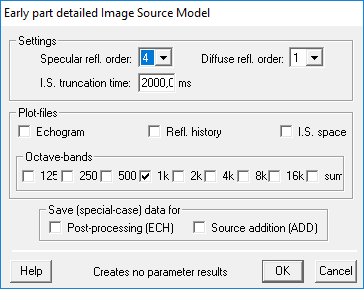
\includegraphics[width=0.6\textwidth]{archivos/capturas/ismcatt.png}
    \caption{Ventana de parámetros para el trazado de rayos en CATT-Acoustic.}
\end{figure}

En las opciones se permite elegir hasta un máximo de 9 reflexiones (\textit{Specular reflection order}), es decir, cada rayo emitido se sigue calculando hasta que se produce la novena reflexión y, si en esa última reflexión no impacta con el receptor, se desecha. Además de este límite de reflexión se debe incluir un tiempo máximo de duración del rayo (\textit{Image Source truncation time}), que teniendo en cuenta la información que se quiere extraer (campo directo, campo temprano y campo tardío) es recomendable que sea mayor que el valor del tiempo de reverberación.

Debido a la arquitectura del programa (32 bits) y, seguramente a los algoritmos utilizados (no conocidos), no es posible calcular para recintos como los de este trabajo rayos reflejados más de 4 veces cuando se incluye el mobiliario. Si se retira el mobiliario permite el máximo de 9 reflexiones pero en ninguno de los casos siguientes (apartados \ref{cattop} y \ref{catteps}) se obtienen más allá de las octavas reflexiones, obteniendo así una reducida densidad de rayos en la historia temporal (recepción de rayos con un espacio temporal grande entre ellos) y tiempo máximo de rayos aproximadamente entre los 300-400 ms (perdiendo toda la cola reverberante o campo tardío).

El programa no ofrece ninguna otra alternativa para analizar los campos acústicos. La opción de obtener la respuesta al impulso en archivo de audio (.wav) para su posterior análisis en el programa dBFA no es viable porque CATT-Acoustic no ofrece los .wav sin normalizar, perdiendo toda referencia con la distancia emisor-receptor.

La historia temporal se obtiene para cada receptor por separado y la tabla de datos\footnote{Desde la primera versión de CATT-Acoustic 8, \textit{build 1}, hasta la \textit{build 2.1} el signo decimal es una coma, en versiones posteriores es un punto.} (obviando otras informaciones contenidas en el archivo de texto) tiene el siguiente formato:

\begin{figure}[H]
    \centering
    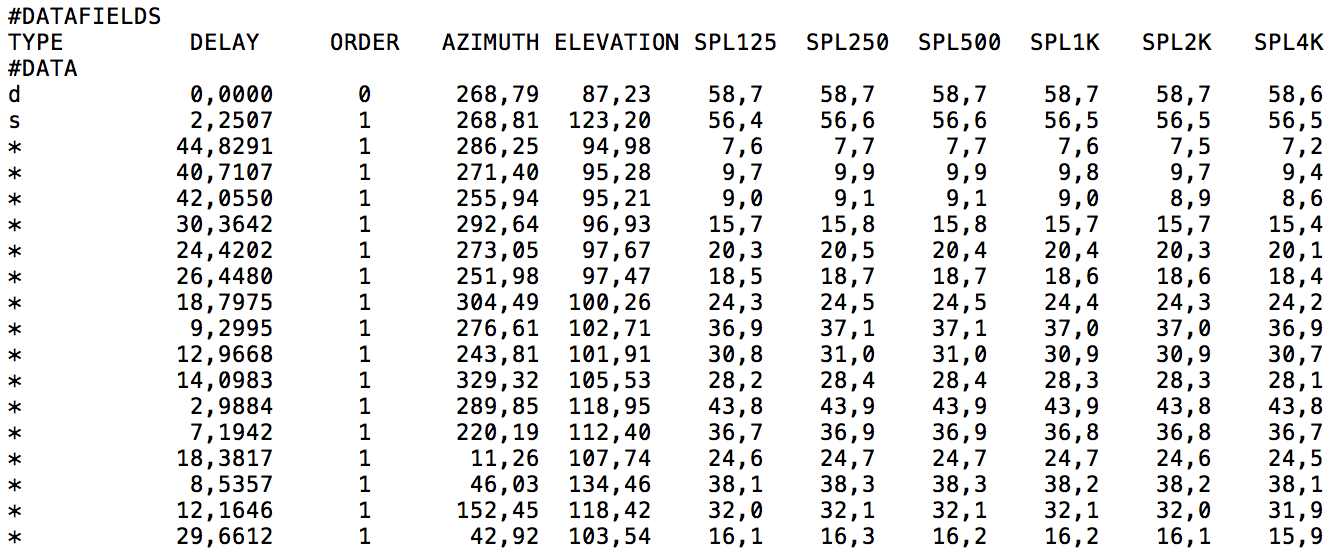
\includegraphics[width=0.8\textwidth]{archivos/capturas/ismtxt.png}
    \caption{Porción de la tabla de datos de un receptor generada por el trazado de rayos en CATT-Acoustic.}
\end{figure}


Adelantando los resultados de la validación de modelos, se ha comprobado que el programa CATT-Acoustic (en su versión 8) no permite cálculos detallados, para ello la opción recomendable es EASE.

\subsubsection{Aula OP/S003}
\label{cattop}

Para la simulación del aula OP/S003 en CATT-Acoustic se han ubicado los puntos de recepción en los mismos lugares que en las medidas in situ, 48 receptores para el caso del aula con mobiliario y 22 sin mobiliario. Las fuentes, una en el centro y otra en la esquina son omnidireccionales con un nivel de presión acústica a 1 metro de 70dB por octava emitiendo ruido rosa.


El tiempo medio de cálculo ha sido:
\begin{itemize}
\itemsep0em
  \item Con mobiliario: 6 horas.
  \item Sin mobiliario: 30 minutos.
\end{itemize}


El modelo tridimensional con mobiliario y sin él se puede observar en la figura \ref{modeloopcatt}.

\begin{figure}[H]
    \centering
    \begin{subfigure}[b]{0.45\textwidth}
    	\centering
        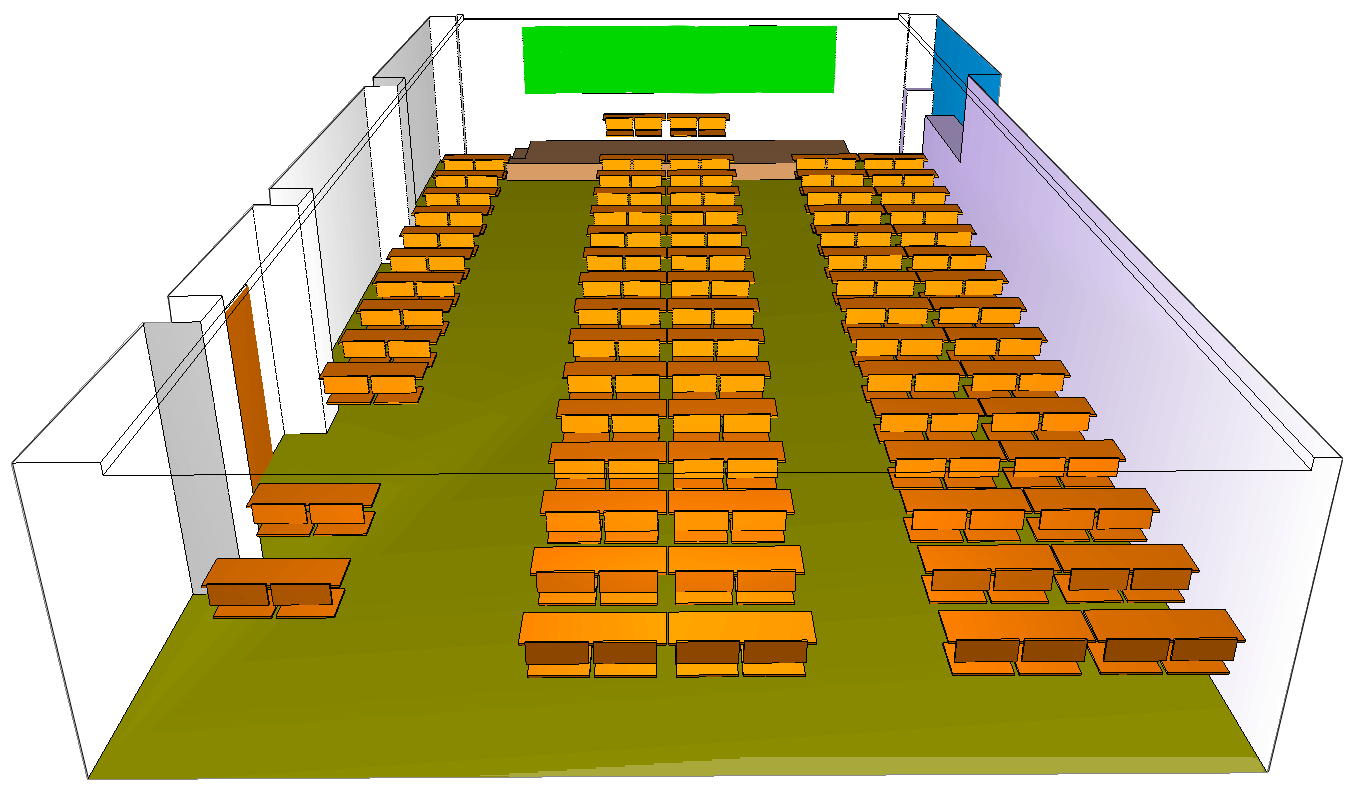
\includegraphics[width=0.9\linewidth]{archivos/capturas/opticallenacatt.png}
    \end{subfigure}
    ~ % Añadir el espacio deseado, si se deja la linea en blanco la siguiente subfigura ira en una nueva linea
    \begin{subfigure}[b]{0.45\textwidth}
    	\centering
        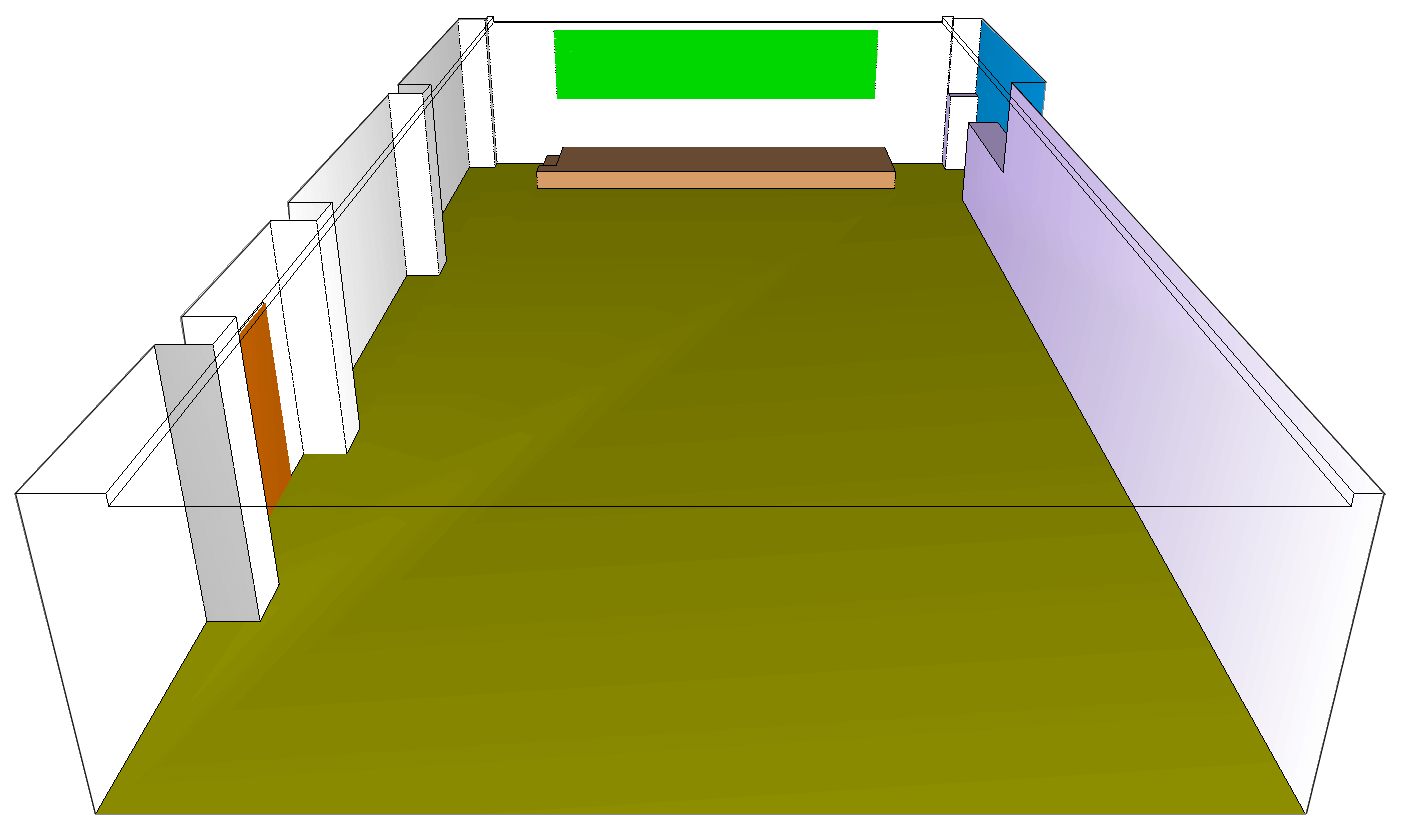
\includegraphics[width=0.9\linewidth]{archivos/capturas/opticavaciacatt.png}
    \end{subfigure}
    \caption{Modelos del Aula OP/S003 en CATT-Acoustic.}\label{modeloopcatt}
\end{figure}

\newpage

Los cálculos del tiempo de reverberación por bandas de octava son:

\begin{table}[H]
\centering
{\scalefont{0.9}
\begin{tabular}{@{}lccccccc@{}}
\toprule
Frecuencia (Hz) & 125 & 250 & 500 & 1000 & 2000 & 4000 & 8000 \\ \midrule
$T30$ Con mobiliario (s) & 1.09 & 1.54 & 1.72 & 1.58 & 1.35 & 1.28 & 1.05 \\
$T30$ Sin mobiliario (s) & 1.24 & 1.87 & 2.10 & 1.85 & 1.67 & 1.62 & 1.31 \\ \bottomrule
\end{tabular}
}
\caption{Tiempos de reverberación calculados en el aula OP/S003 por banda de octava, con y sin mobiliario mediante CATT-Acoustic (T30 extrapolado).}
\label{tab:revopcatt}
\end{table}


Comparando con las medidas in situ se obtiene la desviación entre los resultados:

\begin{table}[H]
\centering
{\scalefont{0.9}
\begin{tabular}{@{}lccccccc@{}}
\toprule
Frecuencia (Hz) & 125 & 250 & 500 & 1000 & 2000 & 4000 & 8000 \\ \midrule
$\sigma_{T30}$ Con mobiliario (s) & 0.02 & 0.01 & 0.01 & 0.11 & 0.01 & 0.01 & 0.02 \\
$\sigma_{T30}$ Sin mobiliario (s) & 0.03 & 0.04 & 0.05 & 0.01 & 0.01 & 0.03 & 0.01 \\ \bottomrule
\end{tabular}
}
\caption{Desviación de los tiempos de reverberación calculados en el aula OP/S003 por banda de octava, con y sin mobiliario mediante CATT-Acoustic (T30 extrapolado) respecto a los medidos in situ.}
\label{tab:desrevopcatt}
\end{table}


Las curvas de los campos acústicos obtenidos se muestran junto a las obtenidas in situ (corrigiendo los niveles de las curvas in situ) en las figuras \ref{graf:cattopmob} y \ref{graf:cattopnomob}.

\begin{figure}[ht]
    \begin{subfigure}[b]{0.4\textwidth}
    	\centering%
         {\scalefont{0.8}%
    %%%%%%%%%%%%%%%%%%%%%%%%%%%%%%%%%%%%%%%%%%%%%%%%%%%%%%%%%%%%%%%%%%%%%%%%
% Escuela Politécnica Superior de la Universidad de Alicante
% Realizado por: Jose Manuel Requena Plens
% Contacto: info@jmrplens.com / Telegram:@jmrplens
%%%%%%%%%%%%%%%%%%%%%%%%%%%%%%%%%%%%%%%%%%%%%%%%%%%%%%%%%%%%%%%%%%%%%%%%

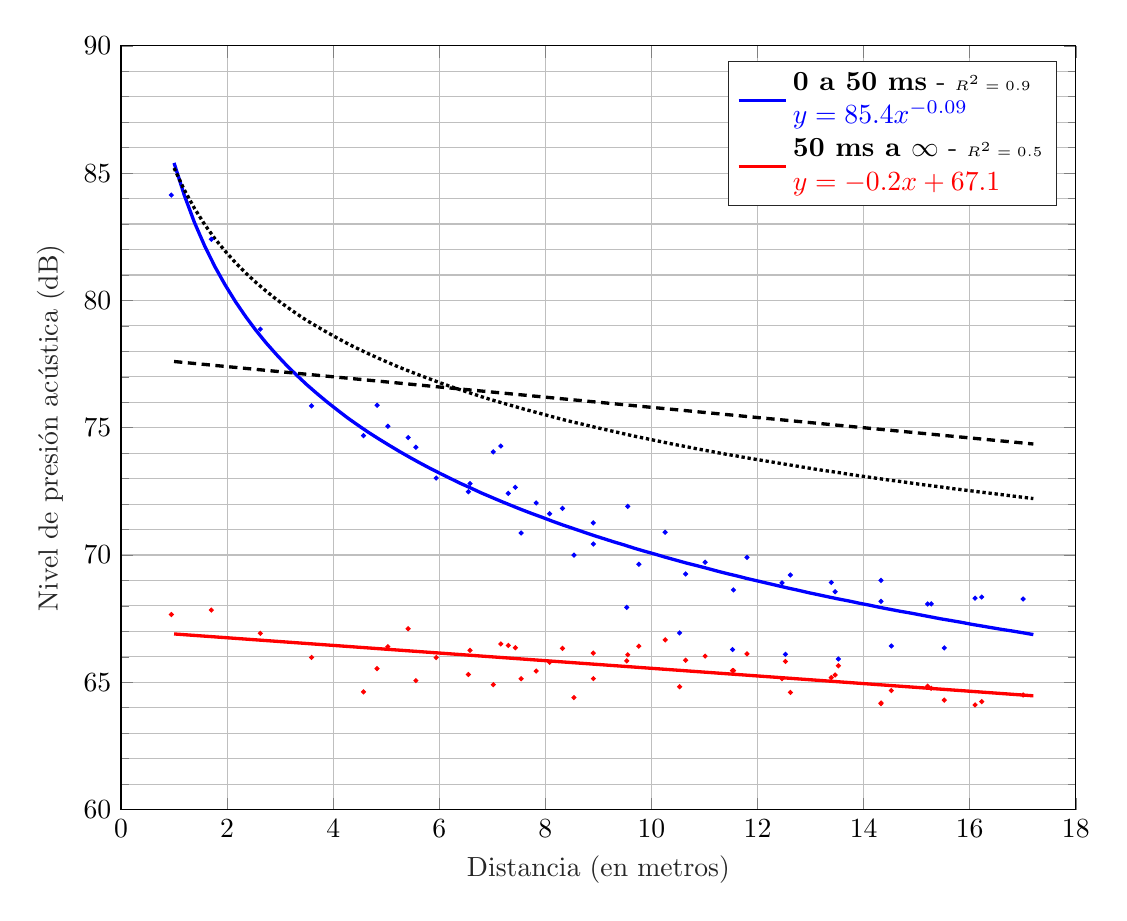
\begin{tikzpicture}

\begin{axis}[%
width=\textwidth,
height=0.8\textwidth,
at={(0\textwidth,0\textwidth)},
scale only axis,
xmin=0,
xmax=18,
xlabel style={font=\color{white!15!black}},
xlabel={Distancia (en metros)},
ymin=60,
ymax=90,
ylabel style={font=\color{white!15!black}},
ylabel={Nivel de presión acústica (dB)},
axis background/.style={fill=white},
xmajorgrids,
xminorgrids,
ymajorgrids,
yminorgrids,
minor y tick num= 4,
legend style={legend cell align=left, align=left, draw=white!15!black}
]
% Curvas CATT
\addplot[color=blue,domain=1:17.2, samples=85,line width=1.2]{85.40*x^(-0.086)};
\addlegendentry{\textbf{0 a 50 ms} - \tiny{$R^2 = 0.9$}\\$\color{blue}y = 85.4·x^{-0.09}$}

\addplot[color=red,domain=1:17.2, samples=85,line width=1.2]{-0.15*x+67.05};
\addlegendentry{\textbf{50 ms a $\infty$} - \tiny{$R^2 = 0.5$}\\$\color{red}y = -0.2·x+67.1$}

% Curvas insitu
\addplot[color=black,densely dotted,line width=1.2pt,domain=1:17.2, samples=85]{82.8*x^(-0.06)+2.4};
\addplot[color=black,densely dashed,line width=1.2pt,domain=1:17.2, samples=85]{-0.2*x+75.4+2.4};

% Puntos
\addplot [color=blue, only marks,mark size=0.7pt]
  table[row sep=crcr]{%
0.948683298050514	84.1353116879552\\
1.70293863659264	82.4012077653756\\
2.62678510731274	78.8706517510003\\
3.59165699921359	75.8564180282084\\
4.57165178026498	74.6880743885206\\
4.82700735445887	75.8827788081102\\
5.02991053598372	75.0582671232784\\
5.41294744108974	74.6118800571909\\
5.55877684387492	74.2348617817552\\
5.94138031100518	73.0212509995305\\
6.54980915752513	72.4847772376713\\
6.58027355054484	72.8066082576771\\
7.01854685814663	74.0512017195111\\
7.15960892786750	74.2806107342639\\
7.30068489937759	72.4207334130398\\
7.43370701601832	72.6594865030346\\
7.54320886625844	70.8652636227284\\
7.82687677173980	72.0454323475206\\
8.08084154033477	71.6233426096783\\
8.32225930862527	71.8328819316278\\
8.53814968245463	69.9956654166565\\
8.90280854562199	71.2657875670075\\
8.90505474435727	70.4310977217243\\
9.53414914924242	67.9411345247112\\
9.55300999685439	71.9083077416819\\
9.76217188949263	69.6363210632465\\
10.2596296229445	70.8940654171431\\
10.5309068935206	66.9413249949675\\
10.6442472725881	69.2568788511997\\
11.0118118400198	69.7171102835565\\
11.5282262295637	66.2877606752058\\
11.5455619178973	68.6288627837818\\
11.8008474271978	69.9071764745151\\
12.4619420637395	68.9069331691573\\
12.5259730160974	66.1006188424368\\
12.6198256723300	69.2152196385029\\
13.3902949930164	68.9211755687166\\
13.4632834033901	68.5577125551089\\
13.5240526470433	65.9156427223462\\
14.3268977800499	69.0019448972321\\
14.3282936876657	68.1806819286096\\
14.5223964964464	66.4262288963540\\
15.2072351201657	68.0774529840046\\
15.2741611880980	68.0818909640558\\
15.5209535789526	66.3504214852306\\
16.1015527201571	68.3051272669117\\
16.2265215003093	68.3507286316659\\
17.0076453396700	68.2712096093625\\
};

\addplot [color=red, only marks,mark size=0.7pt]
  table[row sep=crcr]{%
  0.948683298050514	67.6622769160291\\
1.70293863659264	67.8370730761900\\
2.62678510731274	66.9235042852262\\
3.59165699921359	65.9769203677901\\
4.57165178026498	64.6229239464268\\
4.82700735445887	65.5382279495383\\
5.02991053598372	66.3996653139146\\
5.41294744108974	67.1051572619052\\
5.55877684387492	65.0657727490930\\
5.94138031100518	65.9713330155896\\
6.54980915752513	65.3077891683630\\
6.58027355054484	66.2549011848705\\
7.01854685814663	64.9072387541663\\
7.15960892786750	66.5065489235912\\
7.30068489937759	66.4473915631091\\
7.43370701601832	66.3588935270306\\
7.54320886625844	65.1427315426941\\
7.82687677173980	65.4422299933505\\
8.08084154033477	65.7844640045054\\
8.32225930862527	66.3322698267540\\
8.53814968245463	64.3998896900899\\
8.90280854562199	66.1493978135388\\
8.90505474435727	65.1457503163446\\
9.53414914924242	65.8452828074915\\
9.55300999685439	66.0823577663314\\
9.76217188949263	66.4195520807225\\
10.2596296229445	66.6689251297101\\
10.5309068935206	64.8286246077237\\
10.6442472725881	65.8675704553200\\
11.0118118400198	66.0292842659261\\
11.5282262295637	65.4605432667325\\
11.5455619178973	65.4595750248920\\
11.8008474271978	66.1178808967974\\
12.4619420637395	65.1402626454580\\
12.5259730160974	65.8207053790964\\
12.6198256723300	64.6045872489334\\
13.3902949930164	65.1852845983902\\
13.4632834033901	65.2882424735501\\
13.5240526470433	65.6485563515826\\
14.3268977800499	64.1608691305821\\
14.3282936876657	64.1881410798489\\
14.5223964964464	64.6767123994177\\
15.2072351201657	64.8469050213746\\
15.2741611880980	64.7657920758191\\
15.5209535789526	64.3022766939755\\
16.1015527201571	64.1134715935375\\
16.2265215003093	64.2435874061473\\
17.0076453396700	64.5032386736177\\
  };
\end{axis}
\end{tikzpicture}%%
    }
    \caption{Fuente en la esquina}%
    \end{subfigure}%
    \hspace{1.9cm}%
    \begin{subfigure}[b]{0.4\textwidth}%
    	\centering%
        {\scalefont{0.8}%
    %%%%%%%%%%%%%%%%%%%%%%%%%%%%%%%%%%%%%%%%%%%%%%%%%%%%%%%%%%%%%%%%%%%%%%%%
% Escuela Politécnica Superior de la Universidad de Alicante
% Realizado por: Jose Manuel Requena Plens
% Contacto: info@jmrplens.com / Telegram:@jmrplens
%%%%%%%%%%%%%%%%%%%%%%%%%%%%%%%%%%%%%%%%%%%%%%%%%%%%%%%%%%%%%%%%%%%%%%%%

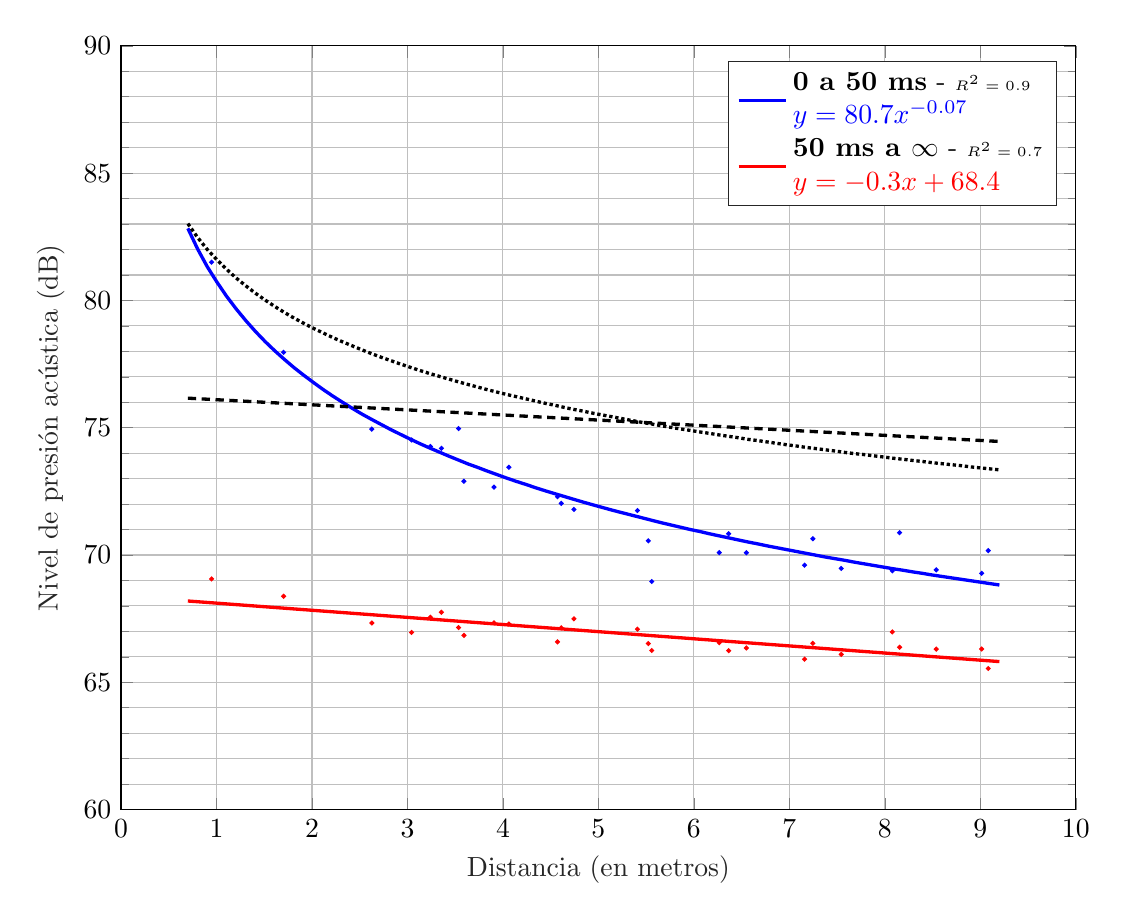
\begin{tikzpicture}

\begin{axis}[%
width=\textwidth,
height=0.8\textwidth,
at={(0\textwidth,0\textwidth)},
scale only axis,
xmin=0,
xmax=10,
xlabel style={font=\color{white!15!black}},
xlabel={Distancia (en metros)},
ymin=60,
ymax=90,
ylabel style={font=\color{white!15!black}},
ylabel={Nivel de presión acústica (dB)},
axis background/.style={fill=white},
xmajorgrids,
xminorgrids,
ymajorgrids,
yminorgrids,
minor y tick num= 4,
legend style={legend cell align=left, align=left, draw=white!15!black}
]
% Curvas CATT
\addplot[color=blue,domain=0.7:9.2, samples=85,line width=1.2]{80.73*x^(-0.072)};
\addlegendentry{\textbf{0 a 50 ms} - \tiny{$R^2 = 0.9$}\\$\color{blue}y = 80.7·x^{-0.07}$}

\addplot[color=red,domain=0.7:9.2, samples=85,line width=1.2]{-0.28*x+68.39};
\addlegendentry{\textbf{50 ms a $\infty$} - \tiny{$R^2 = 0.7$}\\$\color{red}y = -0.3·x+68.4$}

% Curvas in situ
\addplot[color=black,densely dotted,line width=1.2pt,domain=0.7:9.2, samples=85]{78.7*x^(-0.05)+2.9};
\addplot[color=black,densely dashed,line width=1.2pt,domain=0.7:9.2, samples=85]{-0.2*x+73.40+2.9};

% Puntos
\addplot [color=blue, only marks,mark size=0.7pt]
  table[row sep=crcr]{%
  0.948683298050514	81.5034022462516\\
1.70293863659264	77.9604720495982\\
2.62678510731274	74.9450056206266\\
3.04302481094059	74.5164853119413\\
3.24037034920393	74.2620379082671\\
3.35559234711250	74.1888946213408\\
3.53553390593274	74.9657493376305\\
3.59165699921359	72.8967181276975\\
3.90640499692492	72.6674994614721\\
4.06201920231798	73.4447542538069\\
4.57165178026498	72.2893786447318\\
4.61085675335940	72.0269191607698\\
4.74341649025257	71.7920610855486\\
5.40925133451941	71.7470474133201\\
5.52268050859363	70.5575249312815\\
5.55877684387492	68.9590671078746\\
6.26578007912822	70.0965854954904\\
6.36396103067893	70.8361666485416\\
6.54980915752513	70.0912217996624\\
7.15960892786750	69.6020991584691\\
7.24568837309472	70.6388641001404\\
7.54320886625844	69.4711599008487\\
8.07836617144828	69.3786993792196\\
8.15475321515005	70.8779927992126\\
8.53814968245463	69.4178255738047\\
9.01443287178955	69.2818532843703\\
9.08295106229248	70.1712672420559\\
  };
  
  \addplot [color=red, only marks,mark size=0.7pt]
  table[row sep=crcr]{%
  0.948683298050514	69.0614022592804\\
1.70293863659264	68.3789306872370\\
2.62678510731274	67.3305757179527\\
3.04302481094059	66.9599563309559\\
3.24037034920393	67.5537179622664\\
3.35559234711250	67.7505225752068\\
3.53553390593274	67.1500247730451\\
3.59165699921359	66.8427309755973\\
3.90640499692492	67.3393968502688\\
4.06201920231798	67.2906360577647\\
4.57165178026498	66.5896277965778\\
4.61085675335940	67.1423946944337\\
4.74341649025257	67.4933509242810\\
5.40925133451941	67.0859873464819\\
5.52268050859363	66.5216181182482\\
5.55877684387492	66.2501919867704\\
6.26578007912822	66.5596497676022\\
6.36396103067893	66.2436355563401\\
6.54980915752513	66.3492883390880\\
7.15960892786750	65.9096755815499\\
7.24568837309472	66.5306785734246\\
7.54320886625844	66.0974333054611\\
8.07836617144828	66.9797629598969\\
8.15475321515005	66.3778728334517\\
8.53814968245463	66.3054831839590\\
9.01443287178955	66.3088472266783\\
9.08295106229248	65.5428242170173\\
  };
\end{axis}
\end{tikzpicture}%%
    }
    \caption{Fuente en el centro}%
    \end{subfigure}
    \caption{Campos acústicos en el aula OP/S003 con mobiliario simulado en CATT-Acoustic. Se muestran las curvas in situ (líneas discontinuas) con el nivel global modificado para poder comparar.}
    \label{graf:cattopmob}%
\end{figure}
\FloatBarrier 


\begin{figure}[ht]
    \begin{subfigure}[b]{0.4\textwidth}
    	\centering%
         {\scalefont{0.8}%
    %%%%%%%%%%%%%%%%%%%%%%%%%%%%%%%%%%%%%%%%%%%%%%%%%%%%%%%%%%%%%%%%%%%%%%%%
% Escuela Politécnica Superior de la Universidad de Alicante
% Realizado por: Jose Manuel Requena Plens
% Contacto: info@jmrplens.com / Telegram:@jmrplens
%%%%%%%%%%%%%%%%%%%%%%%%%%%%%%%%%%%%%%%%%%%%%%%%%%%%%%%%%%%%%%%%%%%%%%%%

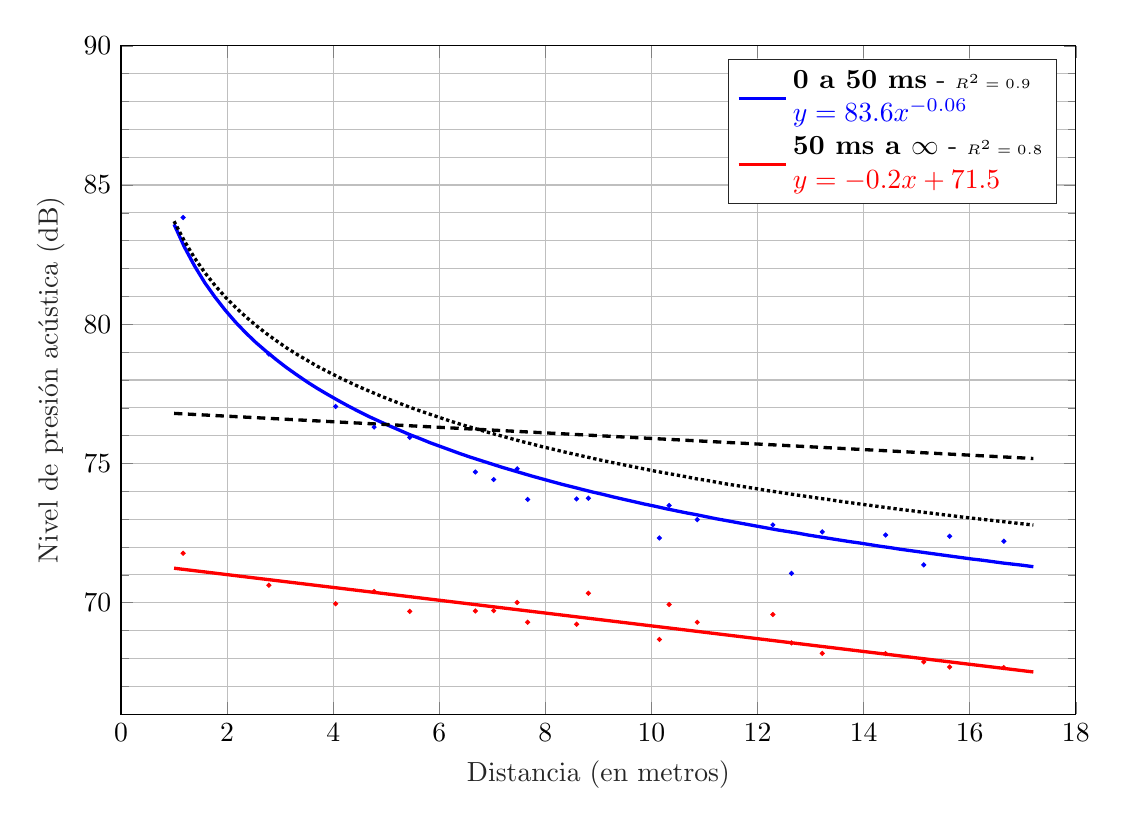
\begin{tikzpicture}

\begin{axis}[%
width=\textwidth,
height=0.7\textwidth,
at={(0\textwidth,0\textwidth)},
scale only axis,
xmin=0,
xmax=18,
xlabel style={font=\color{white!15!black}},
xlabel={Distancia (en metros)},
ymin=66,
ymax=90,
ylabel style={font=\color{white!15!black}},
ylabel={Nivel de presión acústica (dB)},
axis background/.style={fill=white},
xmajorgrids,
xminorgrids,
ymajorgrids,
yminorgrids,
minor y tick num= 4,
legend style={legend cell align=left, align=left, draw=white!15!black}
]
% Curvas CATT
\addplot[color=blue,domain=1:17.2, samples=85,line width=1.2]{83.59*x^(-0.056)};
\addlegendentry{\textbf{0 a 50 ms} - \tiny{$R^2 = 0.9$}\\$\color{blue}y = 83.6·x^{-0.06}$}

\addplot[color=red,domain=1:17.2, samples=85,line width=1.2]{-0.23*x+71.47};
\addlegendentry{\textbf{50 ms a $\infty$} - \tiny{$R^2 = 0.8$}\\$\color{red}y = -0.2·x+71.5$}

% Curvas insitu
\addplot[color=black,densely dotted,line width=1.2pt,domain=1:17.2, samples=85]{82.4*x^(-0.05)+1.3};
\addplot[color=black,densely dashed,line width=1.2pt,domain=1:17.2, samples=85]{-0.1*x+75.6+1.3};

% Puntos
\addplot [color=blue, only marks,mark size=0.7pt]
  table[row sep=crcr]{%
1.17046999107196	83.8329777120332\\
2.78747197295327	78.9306384962613\\
4.04598566482878	77.0498042019777\\
4.77179211617606	76.3062472099297\\
5.44357419348722	75.9377982206261\\
6.68075594525051	74.6944529453703\\
7.02637886823647	74.4249636604886\\
7.46793144049944	74.8080290478306\\
7.66615940350838	73.7111005477617\\
8.58894638474359	73.7286958740670\\
8.81093071133805	73.7544124640849\\
10.1498768465435	72.3277287217195\\
10.3329569823938	73.4949762336248\\
10.8637010268140	72.9838872461474\\
12.2890194889584	72.7960325948105\\
12.6400158227749	71.0558026132494\\
13.2200605142337	72.5464433961370\\
14.4142290810157	72.4316131041346\\
15.1334067545943	71.3605121070253\\
15.6211395230950	72.3863346098596\\
16.6439178080162	72.2106523500810\\
18.4775539506722	72.3500886557943\\
};

\addplot [color=red, only marks,mark size=0.7pt]
  table[row sep=crcr]{%
  1.17046999107196	71.7775654046139\\
2.78747197295327	70.6303063464095\\
4.04598566482878	69.9635797822371\\
4.77179211617606	70.4020975986096\\
5.44357419348722	69.6894116908404\\
6.68075594525051	69.7053811912342\\
7.02637886823647	69.7137208542767\\
7.46793144049944	70.0108618230364\\
7.66615940350838	69.3018030921320\\
8.58894638474359	69.2302641444601\\
8.81093071133805	70.3403117898067\\
10.1498768465435	68.6839446505491\\
10.3329569823938	69.9369892497103\\
10.8637010268140	69.2995548128369\\
12.2890194889584	69.5772033188763\\
12.6400158227749	68.5595087780777\\
13.2200605142337	68.1835354842376\\
14.4142290810157	68.1753790141965\\
15.1334067545943	67.8793448780429\\
15.6211395230950	67.6907594619848\\
16.6439178080162	67.6707394060713\\
18.4775539506722	66.8649481024522\\
  };
\end{axis}
\end{tikzpicture}%%
    }
    \caption{Fuente en la esquina}%
    \label{graf:cattopnomob-a}%
    \end{subfigure}%
    \hspace{1.9cm}%
    \begin{subfigure}[b]{0.4\textwidth}%
    	\centering%
        {\scalefont{0.8}%
    %%%%%%%%%%%%%%%%%%%%%%%%%%%%%%%%%%%%%%%%%%%%%%%%%%%%%%%%%%%%%%%%%%%%%%%%
% Escuela Politécnica Superior de la Universidad de Alicante
% Realizado por: Jose Manuel Requena Plens
% Contacto: info@jmrplens.com / Telegram:@jmrplens
%%%%%%%%%%%%%%%%%%%%%%%%%%%%%%%%%%%%%%%%%%%%%%%%%%%%%%%%%%%%%%%%%%%%%%%%

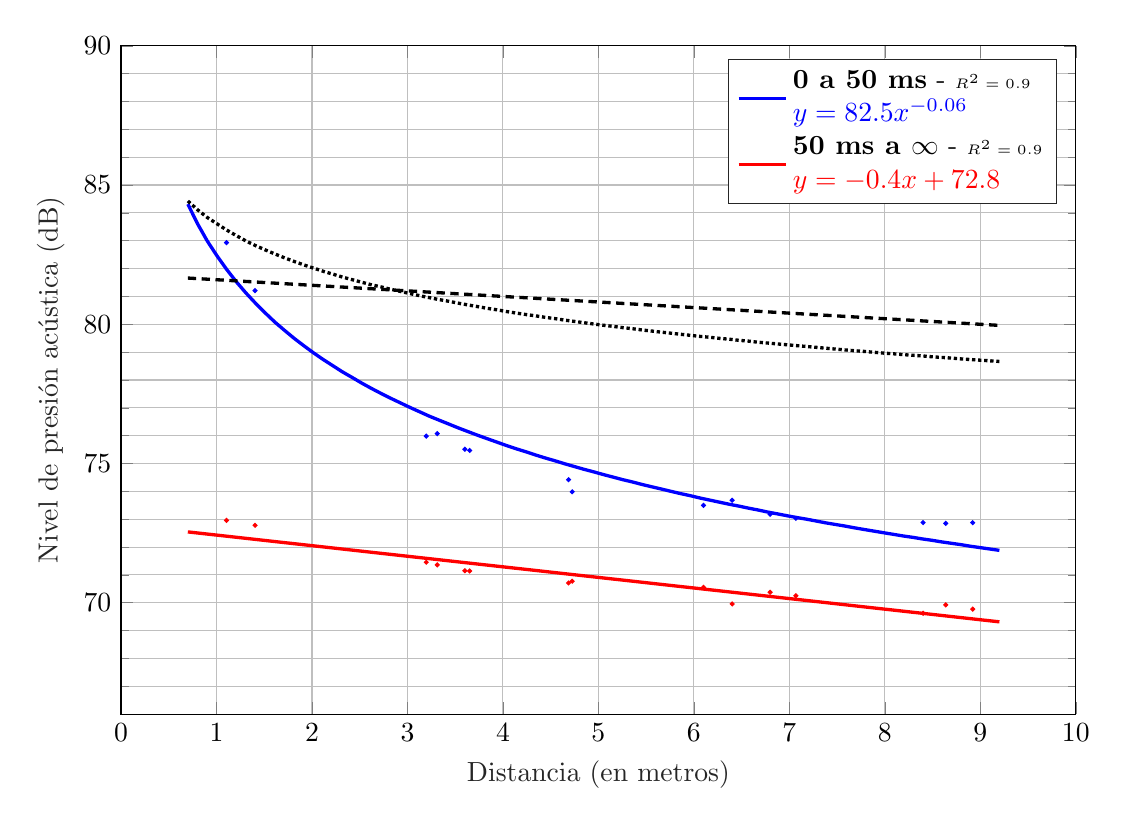
\begin{tikzpicture}

\begin{axis}[%
width=\textwidth,
height=0.7\textwidth,
at={(0\textwidth,0\textwidth)},
scale only axis,
xmin=0,
xmax=10,
xlabel style={font=\color{white!15!black}},
xlabel={Distancia (en metros)},
ymin=66,
ymax=90,
ylabel style={font=\color{white!15!black}},
ylabel={Nivel de presión acústica (dB)},
axis background/.style={fill=white},
xmajorgrids,
xminorgrids,
ymajorgrids,
yminorgrids,
minor y tick num= 4,
legend style={legend cell align=left, align=left, draw=white!15!black}
]
% Curvas CATT
\addplot[color=blue,domain=0.7:9.2, samples=85,line width=1.2]{82.47*x^(-0.062)};
\addlegendentry{\textbf{0 a 50 ms} - \tiny{$R^2 = 0.9$}\\$\color{blue}y = 82.5·x^{-0.06}$}

\addplot[color=red,domain=0.7:9.2, samples=85,line width=1.2]{-0.38*x+72.81};
\addlegendentry{\textbf{50 ms a $\infty$} - \tiny{$R^2 = 0.9$}\\$\color{red}y = -0.4·x+72.8$}

% Curvas in situ
\addplot[color=black,densely dotted,line width=1.2pt,domain=0.7:9.2, samples=85]{76.9*x^(-0.03)+6.7};
\addplot[color=black,densely dashed,line width=1.2pt,domain=0.7:9.2, samples=85]{-0.2*x+75.1+6.7};

% Puntos
\addplot [color=blue, only marks,mark size=0.7pt]
  table[row sep=crcr]{%
  1.10453610171873	82.9345303709531\\
1.40356688476182	81.2102515329224\\
3.19687347262916	75.9856271063767\\
3.31209903233584	76.0756440395286\\
3.60138862107382	75.5150762506015\\
3.65136960605195	75.4708681827389\\
4.68721665810319	74.4180957656198\\
4.72572745722815	73.9855579847906\\
6.10081961706786	73.4964261025427\\
6.40078120232210	73.6785459543595\\
6.79852925271341	73.1772931521972\\
7.06894617322837	73.0315844338110\\
8.40059521700695	72.8777411592766\\
8.63828686719769	72.8483022158284\\
8.92020179143947	72.8746507896277\\
  };
  
  \addplot [color=red, only marks,mark size=0.7pt]
  table[row sep=crcr]{%
  1.10453610171873	72.9562307280560\\
1.40356688476182	72.7819124497572\\
3.19687347262916	71.4545090236686\\
3.31209903233584	71.3575091767311\\
3.60138862107382	71.1480243215088\\
3.65136960605195	71.1422849661127\\
4.68721665810319	70.7100903981730\\
4.72572745722815	70.7730643726906\\
6.10081961706786	70.5520001586585\\
6.40078120232210	69.9591314519951\\
6.79852925271341	70.3752685657530\\
7.06894617322837	70.2508837688623\\
8.40059521700695	69.6209970304835\\
8.63828686719769	69.9245634923070\\
8.92020179143947	69.7722037094251\\
  };
\end{axis}
\end{tikzpicture}%%
    }
    \caption{Fuente en el centro}%
    \end{subfigure}
    \caption{Campos acústicos en el aula OP/S003 sin mobiliario simulado en CATT-Acoustic. Se muestran las curvas in situ (líneas discontinuas) con el nivel global modificado para poder comparar.}
    \label{graf:cattopnomob}%
    \vspace{-0.3cm}
\end{figure}
\FloatBarrier 

Se puede observar claramente que el campo perjudicial obtenido con CATT-Acoustic es inferior al obtenido in situ, esto es debido a la reducida historia temporal que ofrece este programa por lo que la suma energética de este campo es considerablemente menor al que debería obtenerse.

Las curvas de campo útil obtenidas reducen su energía respecto a la distancia en mayor medida de lo medido in situ, existen diferencias notables a excepción de la fuente en esquina sin mobiliario (figura \ref{graf:cattopnomob-a}).

\subsubsection{Aula EP/0-26M}
\label{catteps}

Para la simulación del aula EP/0-26M en CATT-Acoustic se han ubicado los puntos de recepción en los mismos lugares que en las medidas in situ, 30 receptores. Las fuentes, una en el centro y otra en la esquina son omnidireccionales con un nivel de presión acústica a 1 metro de 70dB por octava emitiendo ruido rosa.

El tiempo medio de cálculo ha sido:
\begin{itemize}
\itemsep0em
  \item Con mobiliario: 4 horas.
  \item Sin mobiliario: 20 minutos.
\end{itemize}

El modelo tridimensional con mobiliario y sin él se puede observar en la figura \ref{modeloepscatt}.

\begin{figure}[H]
    \centering
    \begin{subfigure}[b]{0.4\textwidth}
    	\centering
        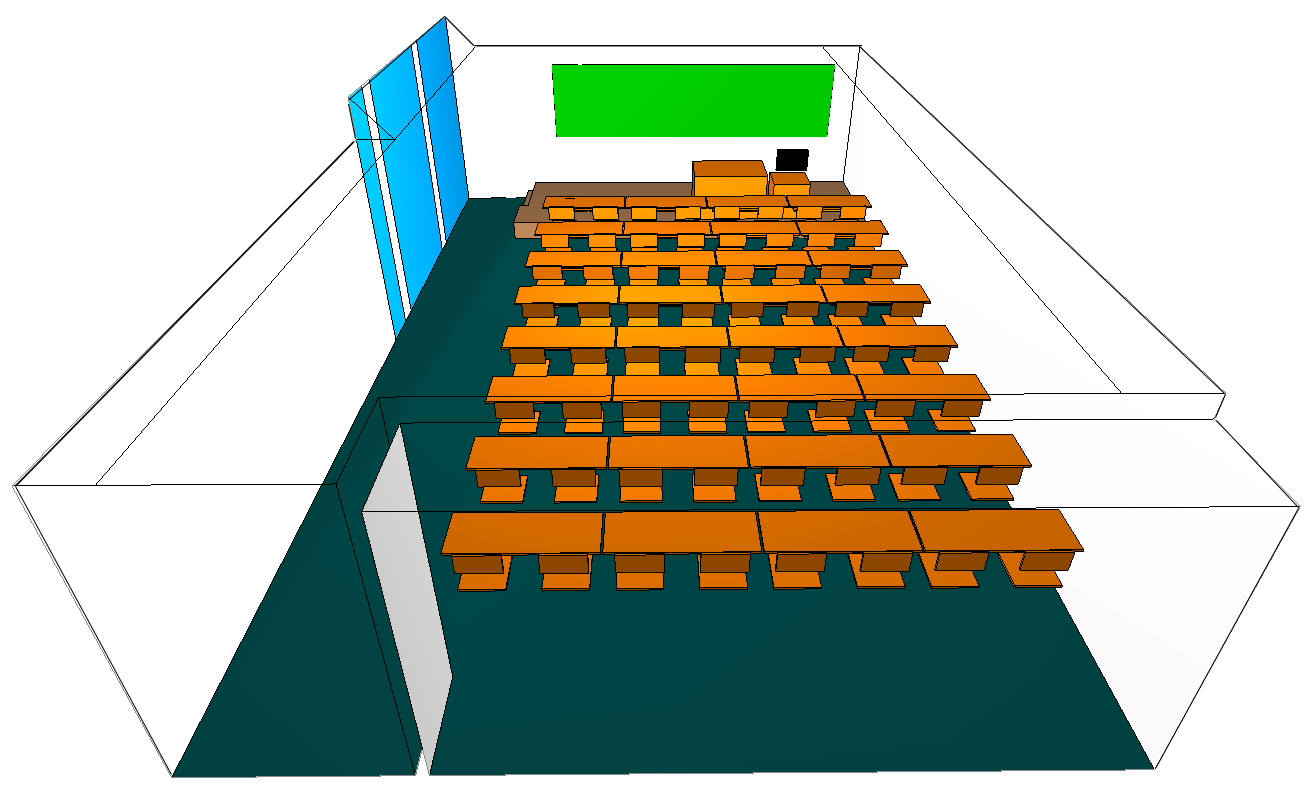
\includegraphics[width=0.9\linewidth]{archivos/capturas/epsllenacatt.png}
    \end{subfigure}
    ~ % Añadir el espacio deseado, si se deja la linea en blanco la siguiente subfigura ira en una nueva linea
    \begin{subfigure}[b]{0.4\textwidth}
    	\centering
        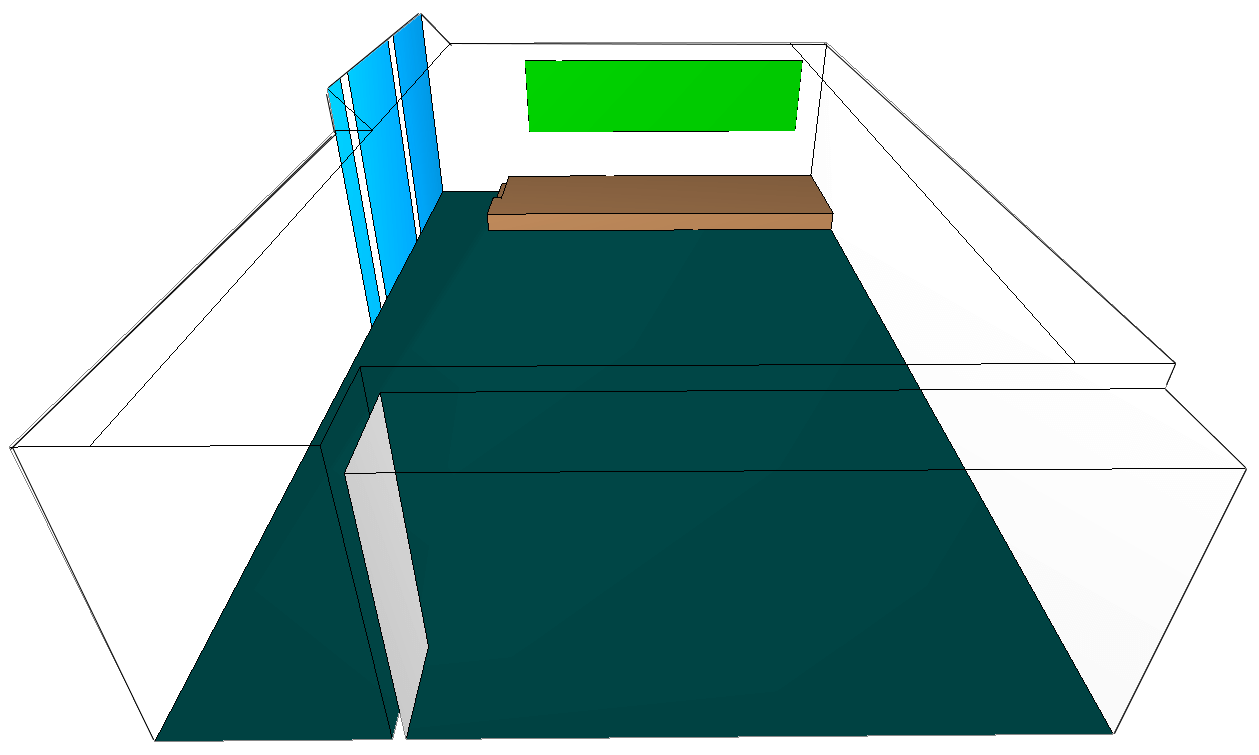
\includegraphics[width=0.9\linewidth]{archivos/capturas/epsvaciacatt.png}
    \end{subfigure}
    \caption{Modelos del Aula EP/0-26M en CATT-Acoustic.}\label{modeloepscatt}
    \vspace{-0.3cm}
\end{figure}


Los cálculos del tiempo de reverberación por bandas de octava son:

\begin{table}[ht]
\centering
{\scalefont{0.9}
\begin{tabular}{@{}lccccccc@{}}
\toprule
Frecuencia (Hz) & 125 & 250 & 500 & 1000 & 2000 & 4000 & 8000 \\ \midrule
$T30$ Con mobiliario (s) & 1.32 & 1.46 & 1.44 & 1.28 & 1.15 & 1.02 & 0.77 \\
$T30$ Sin mobiliario (s) & 1.31 & 1.56 & 1.54 & 1.46 & 1.31 & 1.16 & 0.89 \\ \bottomrule
\end{tabular}
}
\caption{Tiempos de reverberación calculados en el aula EP/0-26M por banda de octava, con y sin mobiliario mediante CATT-Acoustic (T30 extrapolado).}
\label{tab:revepscatt}
\vspace{-0.3cm}
\end{table}
\FloatBarrier

Comparando con las medidas in situ se obtiene la desviación entre los resultados:

\begin{table}[ht]
\centering
{\scalefont{0.9}
\begin{tabular}{@{}lccccccc@{}}
\toprule
Frecuencia (Hz) & 125 & 250 & 500 & 1000 & 2000 & 4000 & 8000 \\ \midrule
$\sigma_{T30}$ Con mobiliario (s) & 0.01 & 0.03 & 0.01 & 0.00 & 0.01 & 0.02 & 0.01 \\
$\sigma_{T30}$ Sin mobiliario (s) & 0.00 & 0.01 & 0.02 & 0.02 & 0.01 & 0.00 & 0.04 \\ \bottomrule
\end{tabular}
}
\caption{Desviación de los tiempos de reverberación calculados en el aula EP/0-26M por banda de octava, con y sin mobiliario mediante CATT-Acoustic (T30 extrapolado) respecto a los medidos in situ.}
\label{tab:desrevepscatt}
\vspace{-0.3cm}
\end{table}
\FloatBarrier

Las curvas de los campos acústicos obtenidos se muestran junto a las obtenidas in situ (corrigiendo los niveles de las curvas in situ) en las figuras \ref{graf:cattepsmob} y \ref{graf:cattepsnomob}.

\begin{figure}[ht]
    \begin{subfigure}[b]{0.4\textwidth}
    	\centering%
         {\scalefont{0.8}%
    %%%%%%%%%%%%%%%%%%%%%%%%%%%%%%%%%%%%%%%%%%%%%%%%%%%%%%%%%%%%%%%%%%%%%%%%
% Escuela Politécnica Superior de la Universidad de Alicante
% Realizado por: Jose Manuel Requena Plens
% Contacto: info@jmrplens.com / Telegram:@jmrplens
%%%%%%%%%%%%%%%%%%%%%%%%%%%%%%%%%%%%%%%%%%%%%%%%%%%%%%%%%%%%%%%%%%%%%%%%

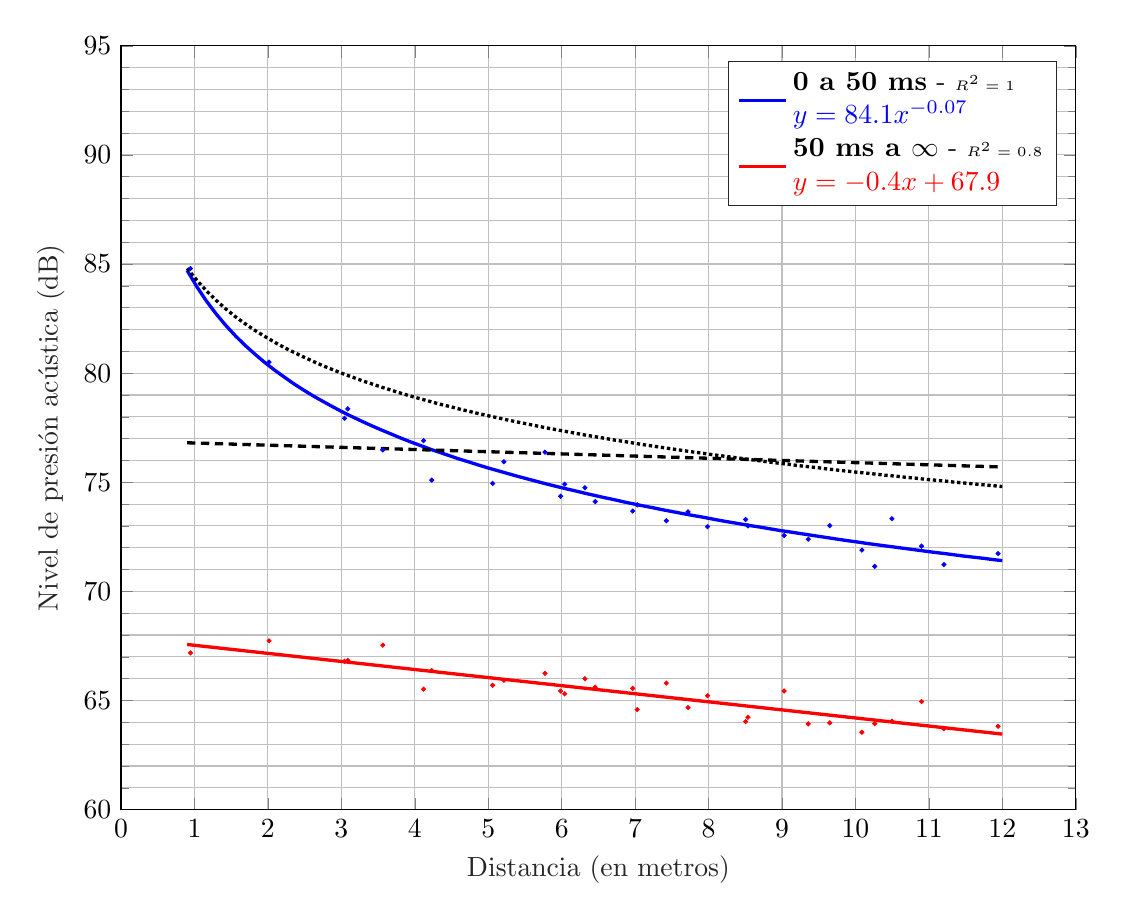
\begin{tikzpicture}

\begin{axis}[%
width=\textwidth,
height=0.8\textwidth,
at={(0\textwidth,0\textwidth)},
scale only axis,
xmin=0,
xmax=13,
xlabel style={font=\color{white!15!black}},
xlabel={Distancia (en metros)},
ymin=60,
ymax=95,
ylabel style={font=\color{white!15!black}},
ylabel={Nivel de presión acústica (dB)},
axis background/.style={fill=white},
xmajorgrids,
xminorgrids,
ymajorgrids,
yminorgrids,
minor y tick num= 4,
legend style={legend cell align=left, align=left, draw=white!15!black}
]
% Curvas CATT
\addplot[color=blue,domain=0.9:12, samples=85,line width=1.2]{84.12*x^(-0.066)};
\addlegendentry{\textbf{0 a 50 ms} - \tiny{$R^2 = 1$}\\$\color{blue}y = 84.1·x^{-0.07}$}

\addplot[color=red,domain=0.9:12, samples=85,line width=1.2]{-0.37*x+67.90};
\addlegendentry{\textbf{50 ms a $\infty$} - \tiny{$R^2 = 0.8$}\\$\color{red}y = -0.4·x+67.9$}

% Curvas insitu
\addplot[color=black,densely dotted,line width=1.2pt,domain=0.9:12, samples=85]{81.97*x^(-0.05)+2.4};
\addplot[color=black,densely dashed,line width=1.2pt,domain=0.9:12, samples=85]{-0.1*x+74.5+2.4};

% Puntos
\addplot [color=blue, only marks,mark size=0.7pt]
  table[row sep=crcr]{%
0.945832966226067	84.7940935165369\\
2.01558924386890	80.5088235545069\\
3.04292622322658	77.9320485825873\\
3.08781476128346	78.3616138191973\\
3.56407070636933	76.4849962017409\\
4.11885906532379	76.9044290192008\\
4.23076825174814	75.1022096058502\\
5.06013833802990	74.9474852055735\\
5.21338661524349	75.9406891324395\\
5.77252977471749	76.3776545896168\\
5.98493107729738	74.3602183547266\\
6.04070360140274	74.9122872758019\\
6.31685048105462	74.7501811500246\\
6.45653932071973	74.1155853234564\\
6.96725196903342	73.6833614278601\\
7.02797979507625	73.9633176156507\\
7.42526767194288	73.2387823461144\\
7.72055049850721	73.6464493382804\\
7.98590007450632	72.9621217488370\\
8.50471045950419	73.2968676723003\\
8.53670896774630	73.0050897339140\\
9.02858792946051	72.5619891945293\\
9.35746226281464	72.3907342162342\\
9.65012953280939	73.0123999306724\\
10.0878639959111	71.8925474764897\\
10.2617201287114	71.1459792238528\\
10.4960706933595	73.3329239412387\\
10.8998853204976	72.0721983743662\\
11.2050211958746	71.2291923307644\\
11.9413148354777	71.7342752766105\\
};

\addplot [color=red, only marks,mark size=0.7pt]
  table[row sep=crcr]{%
  0.945832966226067	67.1862432314636\\
2.01558924386890	67.7363957642089\\
3.04292622322658	66.7922341841050\\
3.08781476128346	66.8344756940026\\
3.56407070636933	67.5344637049481\\
4.11885906532379	65.5179134201327\\
4.23076825174814	66.3756626286794\\
5.06013833802990	65.6982324109378\\
5.21338661524349	65.9286727464098\\
5.77252977471749	66.2406231846175\\
5.98493107729738	65.4331827767847\\
6.04070360140274	65.3071138692085\\
6.31685048105462	65.9984866884834\\
6.45653932071973	65.6090330277700\\
6.96725196903342	65.5561800680073\\
7.02797979507625	64.5839958259255\\
7.42526767194288	65.7967135810376\\
7.72055049850721	64.6762052953775\\
7.98590007450632	65.2183158773717\\
8.50471045950419	64.0318973024421\\
8.53670896774630	64.2315139481329\\
9.02858792946051	65.4339102155443\\
9.35746226281464	63.9297884883784\\
9.65012953280939	63.9747490631797\\
10.0878639959111	63.5461739245062\\
10.2617201287114	63.9410034698324\\
10.4960706933595	64.0533360097354\\
10.8998853204976	64.9527891169313\\
11.2050211958746	63.7054392036513\\
11.9413148354777	63.8179364275073\\
  };
\end{axis}
\end{tikzpicture}%%
    }
    \caption{Fuente en la esquina}%
    \end{subfigure}%
    \hspace{1.9cm}%
    \begin{subfigure}[b]{0.4\textwidth}%
    	\centering%
        {\scalefont{0.8}%
    %%%%%%%%%%%%%%%%%%%%%%%%%%%%%%%%%%%%%%%%%%%%%%%%%%%%%%%%%%%%%%%%%%%%%%%%
% Escuela Politécnica Superior de la Universidad de Alicante
% Realizado por: Jose Manuel Requena Plens
% Contacto: info@jmrplens.com / Telegram:@jmrplens
%%%%%%%%%%%%%%%%%%%%%%%%%%%%%%%%%%%%%%%%%%%%%%%%%%%%%%%%%%%%%%%%%%%%%%%%

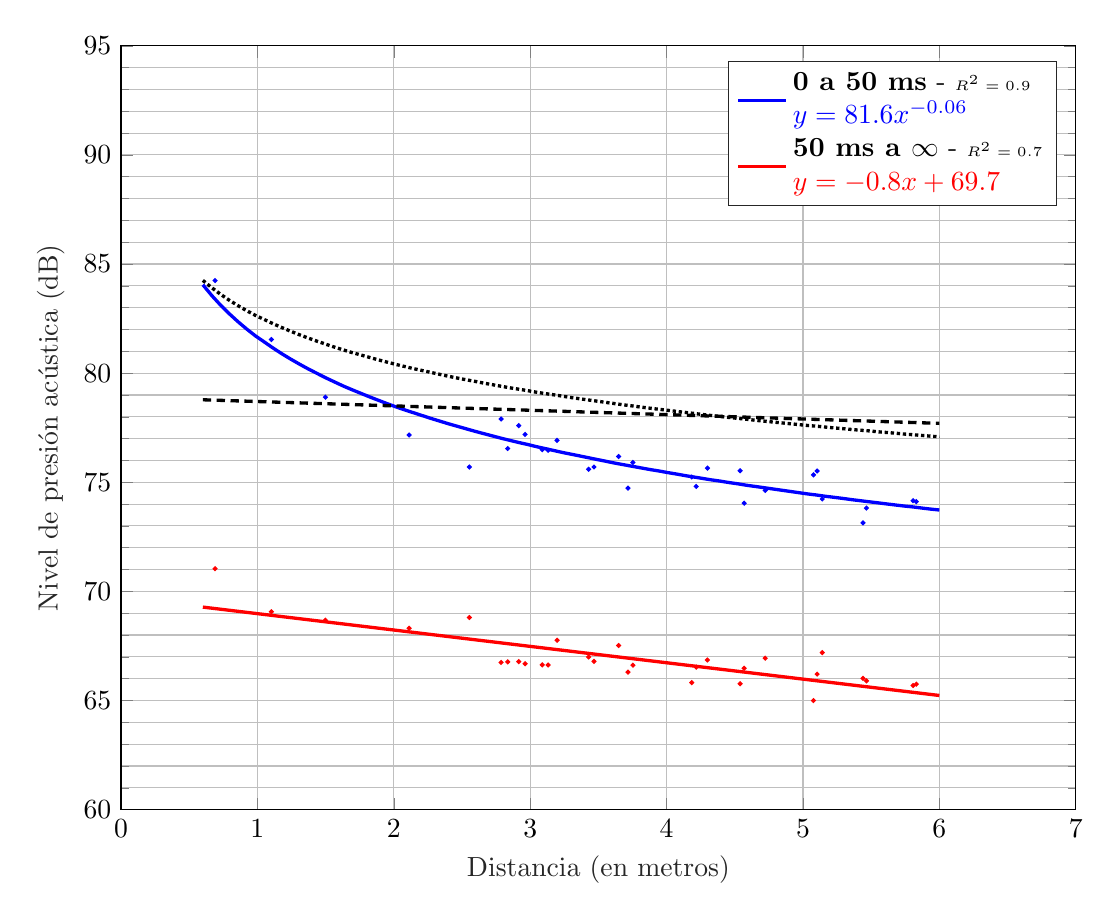
\begin{tikzpicture}

\begin{axis}[%
width=\textwidth,
height=0.8\textwidth,
at={(0\textwidth,0\textwidth)},
scale only axis,
xmin=0,
xmax=7,
xlabel style={font=\color{white!15!black}},
xlabel={Distancia (en metros)},
ymin=60,
ymax=95,
ylabel style={font=\color{white!15!black}},
ylabel={Nivel de presión acústica (dB)},
axis background/.style={fill=white},
xmajorgrids,
xminorgrids,
ymajorgrids,
yminorgrids,
minor y tick num= 4,
legend style={legend cell align=left, align=left, draw=white!15!black}
]
% Curvas CATT
\addplot[color=blue,domain=0.6:6, samples=85,line width=1.2]{81.64*x^(-0.057)};
\addlegendentry{\textbf{0 a 50 ms} - \tiny{$R^2 = 0.9$}\\$\color{blue}y = 81.6·x^{-0.06}$}

\addplot[color=red,domain=0.6:6, samples=85,line width=1.2]{-0.75*x+69.73};
\addlegendentry{\textbf{50 ms a $\infty$} - \tiny{$R^2 = 0.7$}\\$\color{red}y = -0.8·x+69.7$}

% Curvas in situ
\addplot[color=black,densely dotted,line width=1.2pt,domain=0.6:6, samples=85]{80*x^(-0.04)+2.6};
\addplot[color=black,densely dashed,line width=1.2pt,domain=0.6:6, samples=85]{-0.2*x+76.3+2.6};

% Puntos
\addplot [color=blue, only marks,mark size=0.7pt]
  table[row sep=crcr]{%
  0.689492567037528	84.2437937992165\\
1.10208892563168	81.5393902963155\\
1.49833240637717	78.8999701725506\\
2.11248668634858	77.1671995855872\\
2.55409475157051	75.6980857527422\\
2.78664673039121	77.9004908042132\\
2.83511904511962	76.5463502303441\\
2.91626473421053	77.5965680111709\\
2.96261708629381	77.1937172256022\\
3.08787953132890	76.4948784823231\\
3.13169283295792	76.4652759064856\\
3.19677962956473	76.9194649540383\\
3.42820652820101	75.5940050854870\\
3.46772259559498	75.7004739257845\\
3.64836949883095	76.1781249577737\\
3.71663826596025	74.7316905927322\\
3.75311870315875	75.9080742218414\\
4.18442349673166	75.2421231244596\\
4.21685902064558	74.8109591652623\\
4.29941856534113	75.6471178532907\\
4.53878838458019	75.5271639080347\\
4.56870878914382	74.0421073580347\\
4.72298634340605	74.6273479952535\\
5.07690850813760	75.3384191739991\\
5.10367514640186	75.5170973612925\\
5.14125471067132	74.2343403316757\\
5.44027572830643	73.1390003474239\\
5.46526303118157	73.8180774816558\\
5.80710771382794	74.1560949527144\\
5.83052313261855	74.1148027766164\\
  };
  
  \addplot [color=red, only marks,mark size=0.7pt]
  table[row sep=crcr]{%
  0.689492567037528	71.0395734335463\\
1.10208892563168	69.0676151450883\\
1.49833240637717	68.6815339854954\\
2.11248668634858	68.3108210285205\\
2.55409475157051	68.8026922199806\\
2.78664673039121	66.7466126851285\\
2.83511904511962	66.7705919141958\\
2.91626473421053	66.7794866557689\\
2.96261708629381	66.6858262011128\\
3.08787953132890	66.6329756090871\\
3.13169283295792	66.6259180463120\\
3.19677962956473	67.7610977560242\\
3.42820652820101	66.9957746415959\\
3.46772259559498	66.7954120024969\\
3.64836949883095	67.5199448784881\\
3.71663826596025	66.2988226435235\\
3.75311870315875	66.6191248667494\\
4.18442349673166	65.8166902804513\\
4.21685902064558	66.5291153600271\\
4.29941856534113	66.8566107058303\\
4.53878838458019	65.7694182541312\\
4.56870878914382	66.4759244365895\\
4.72298634340605	66.9379988200219\\
5.07690850813760	64.9986267387640\\
5.10367514640186	66.2076076972236\\
5.14125471067132	67.1964069730784\\
5.44027572830643	66.0152128544698\\
5.46526303118157	65.9007581268275\\
5.80710771382794	65.6862291357708\\
5.83052313261855	65.7463302660988\\
  };
\end{axis}
\end{tikzpicture}%%
    }
    \caption{Fuente en el centro}%
    \end{subfigure}
    \caption{Campos acústicos en el aula EP/0-26M con mobiliario simulado en CATT-Acoustic. Se muestran las curvas in situ (líneas discontinuas) con el nivel global modificado para poder comparar.}
    \label{graf:cattepsmob}%
    \vspace{-0.3cm}%
\end{figure}
\FloatBarrier

Al igual que ocurre en el caso del aula OP/S003 (apartado \ref{cattop}) los campos perjudiciales quedan muy por debajo de los medidos in situ y los campos útiles reducen su energía con la distancia en mayor medida que in situ a excepción, al igual que en el otro aula, de la fuente en esquina sin mobiliario (figura \ref{graf:cattepsnomob-a}).

\begin{figure}[H]
    \begin{subfigure}[b]{0.4\textwidth}
    	\centering%
         {\scalefont{0.8}%
    %%%%%%%%%%%%%%%%%%%%%%%%%%%%%%%%%%%%%%%%%%%%%%%%%%%%%%%%%%%%%%%%%%%%%%%%
% Escuela Politécnica Superior de la Universidad de Alicante
% Realizado por: Jose Manuel Requena Plens
% Contacto: info@jmrplens.com / Telegram:@jmrplens
%%%%%%%%%%%%%%%%%%%%%%%%%%%%%%%%%%%%%%%%%%%%%%%%%%%%%%%%%%%%%%%%%%%%%%%%

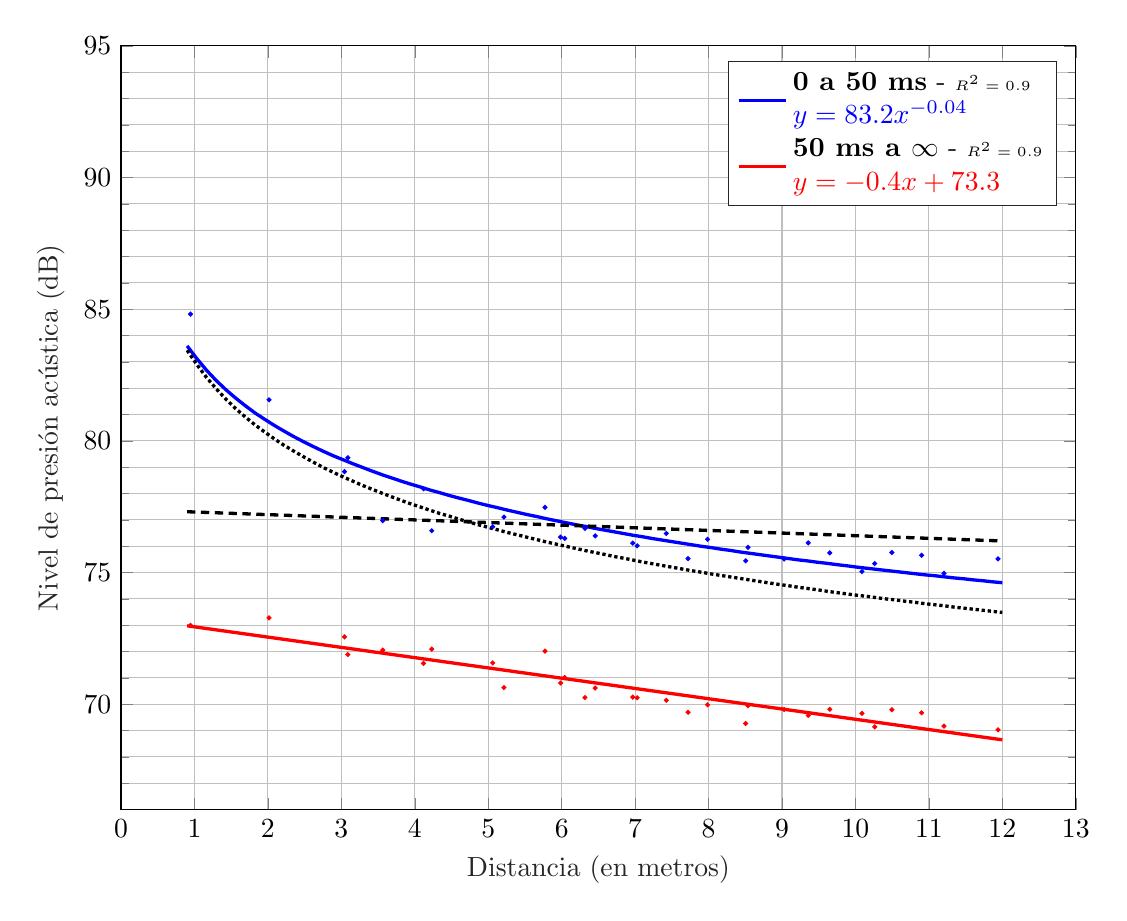
\begin{tikzpicture}

\begin{axis}[%
width=\textwidth,
height=0.8\textwidth,
at={(0\textwidth,0\textwidth)},
scale only axis,
xmin=0,
xmax=13,
xlabel style={font=\color{white!15!black}},
xlabel={Distancia (en metros)},
ymin=66,
ymax=95,
ylabel style={font=\color{white!15!black}},
ylabel={Nivel de presión acústica (dB)},
axis background/.style={fill=white},
xmajorgrids,
xminorgrids,
ymajorgrids,
yminorgrids,
minor y tick num= 4,
legend style={legend cell align=left, align=left, draw=white!15!black}
]
% Curvas CATT
\addplot[color=blue,domain=0.9:12, samples=85,line width=1.2]{83.22*x^(-0.044)};
\addlegendentry{\textbf{0 a 50 ms} - \tiny{$R^2 = 0.9$}\\$\color{blue}y = 83.2·x^{-0.04}$}

\addplot[color=red,domain=0.9:12, samples=85,line width=1.2]{-0.39*x+73.33};
\addlegendentry{\textbf{50 ms a $\infty$} - \tiny{$R^2 = 0.9$}\\$\color{red}y = -0.4·x+73.3$}

% Curvas insitu
\addplot[color=black,densely dotted,line width=1.2pt,domain=0.9:12, samples=85]{81.61*x^(-0.05)+1.4};
\addplot[color=black,densely dashed,line width=1.2pt,domain=0.9:12, samples=85]{-0.1*x+76+1.4};

% Puntos
\addplot [color=blue, only marks,mark size=0.7pt]
  table[row sep=crcr]{%
0.945832966226067	84.8110401658546\\
2.01558924386890	81.5598853737672\\
3.04292622322658	78.8321043919063\\
3.08781476128346	79.3598110886149\\
3.56407070636933	76.9718843715315\\
4.11885906532379	78.1820386335481\\
4.23076825174814	76.5884908271760\\
5.06013833802990	76.7371426398944\\
5.21338661524349	77.1057184165874\\
5.77252977471749	77.4747516242102\\
5.98493107729738	76.3459799299704\\
6.04070360140274	76.2990729247964\\
6.31685048105462	76.6777605068003\\
6.45653932071973	76.3926269496142\\
6.96725196903342	76.1180306246910\\
7.02797979507625	76.0152031225678\\
7.42526767194288	76.4869793946589\\
7.72055049850721	75.5309422973214\\
7.98590007450632	76.2630521086730\\
8.50471045950419	75.4450432338723\\
8.53670896774630	75.9598356404262\\
9.02858792946051	75.5172224330250\\
9.35746226281464	76.1298425135389\\
9.65012953280939	75.7474172478851\\
10.0878639959111	75.0381037317908\\
10.2617201287114	75.3413655416196\\
10.4960706933595	75.7643949335265\\
10.8998853204976	75.6578998745021\\
11.2050211958746	74.9682967699880\\
11.9413148354777	75.5198114175612\\
};

\addplot [color=red, only marks,mark size=0.7pt]
  table[row sep=crcr]{%
  0.945832966226067	72.9936285960842\\
2.01558924386890	73.2794915797714\\
3.04292622322658	72.5607578799376\\
3.08781476128346	71.8866162121520\\
3.56407070636933	72.0571591198002\\
4.11885906532379	71.5542992669876\\
4.23076825174814	72.0928530679978\\
5.06013833802990	71.5706139937870\\
5.21338661524349	70.6327245217427\\
5.77252977471749	72.0178318378904\\
5.98493107729738	70.8065777468409\\
6.04070360140274	71.0183188430378\\
6.31685048105462	70.2552245323064\\
6.45653932071973	70.6155926329650\\
6.96725196903342	70.2722368743506\\
7.02797979507625	70.2441071336058\\
7.42526767194288	70.1491037662452\\
7.72055049850721	69.6943625841994\\
7.98590007450632	69.9799164760509\\
8.50471045950419	69.2708328985608\\
8.53670896774630	69.9449861954152\\
9.02858792946051	69.8010073803832\\
9.35746226281464	69.5748094116539\\
9.65012953280939	69.8096955059744\\
10.0878639959111	69.6538557475760\\
10.2617201287114	69.1410939650944\\
10.4960706933595	69.7932447687360\\
10.8998853204976	69.6765414811656\\
11.2050211958746	69.1685393895153\\
11.9413148354777	69.0299202332542\\
  };
\end{axis}
\end{tikzpicture}%%
    }
    \caption{Fuente en la esquina}%
    \label{graf:cattepsnomob-a}
    \end{subfigure}%
    \hspace{1.9cm}%
    \begin{subfigure}[b]{0.4\textwidth}%
    	\centering%
        {\scalefont{0.8}%
    %%%%%%%%%%%%%%%%%%%%%%%%%%%%%%%%%%%%%%%%%%%%%%%%%%%%%%%%%%%%%%%%%%%%%%%%
% Escuela Politécnica Superior de la Universidad de Alicante
% Realizado por: Jose Manuel Requena Plens
% Contacto: info@jmrplens.com / Telegram:@jmrplens
%%%%%%%%%%%%%%%%%%%%%%%%%%%%%%%%%%%%%%%%%%%%%%%%%%%%%%%%%%%%%%%%%%%%%%%%

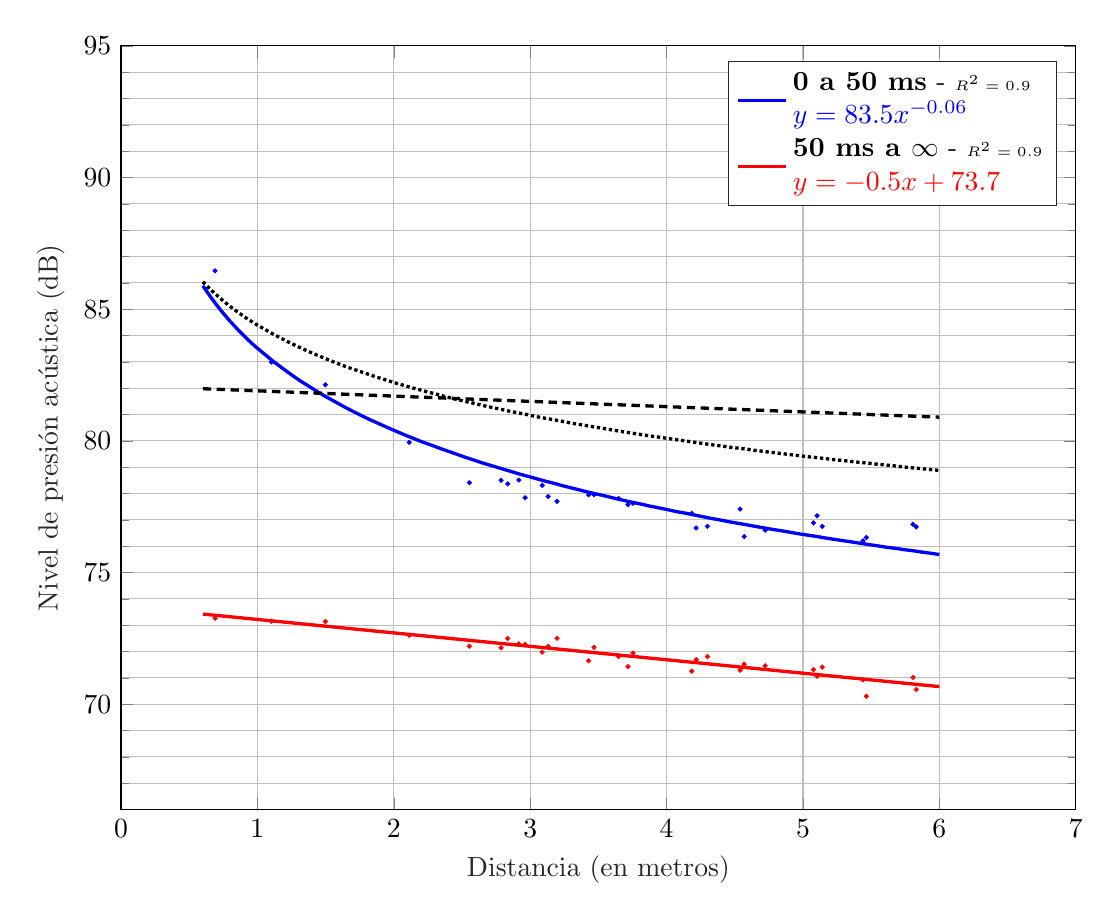
\begin{tikzpicture}

\begin{axis}[%
width=\textwidth,
height=0.8\textwidth,
at={(0\textwidth,0\textwidth)},
scale only axis,
xmin=0,
xmax=7,
xlabel style={font=\color{white!15!black}},
xlabel={Distancia (en metros)},
ymin=66,
ymax=95,
ylabel style={font=\color{white!15!black}},
ylabel={Nivel de presión acústica (dB)},
axis background/.style={fill=white},
xmajorgrids,
xminorgrids,
ymajorgrids,
yminorgrids,
minor y tick num= 4,
legend style={legend cell align=left, align=left, draw=white!15!black}
]
% Curvas CATT
\addplot[color=blue,domain=0.6:6, samples=85,line width=1.2]{83.51*x^(-0.055)};
\addlegendentry{\textbf{0 a 50 ms} - \tiny{$R^2 = 0.9$}\\$\color{blue}y = 83.5·x^{-0.06}$}

\addplot[color=red,domain=0.6:6, samples=85,line width=1.2]{-0.51*x+73.73};
\addlegendentry{\textbf{50 ms a $\infty$} - \tiny{$R^2 = 0.9$}\\$\color{red}y = -0.5·x+73.7$}

% Curvas in situ
\addplot[color=black,densely dotted,line width=1.2pt,domain=0.6:6, samples=85]{79.89*x^(-0.04)+4.5};
\addplot[color=black,densely dashed,line width=1.2pt,domain=0.6:6, samples=85]{-0.2*x+77.6+4.5};

% Puntos
\addplot [color=blue, only marks,mark size=0.7pt]
  table[row sep=crcr]{%
 0.689492567037528	86.4561077651929\\
1.10208892563168	82.9927609595587\\
1.49833240637717	82.1305041957046\\
2.11248668634858	79.9426328135270\\
2.55409475157051	78.4138757021845\\
2.78664673039121	78.5023978482795\\
2.83511904511962	78.3688011736995\\
2.91626473421053	78.5131498025514\\
2.96261708629381	77.8416573473490\\
3.08787953132890	78.3110323572655\\
3.13169283295792	77.8862129133746\\
3.19677962956473	77.7032806606817\\
3.42820652820101	77.9502466641942\\
3.46772259559498	77.9608285992552\\
3.64836949883095	77.8091437262036\\
3.71663826596025	77.5782848169878\\
3.75311870315875	77.6297890568976\\
4.18442349673166	77.2494678783873\\
4.21685902064558	76.6911319691534\\
4.29941856534113	76.7570901918132\\
4.53878838458019	77.4103047718116\\
4.56870878914382	76.3668371688729\\
4.72298634340605	76.6090840131818\\
5.07690850813760	76.8861903015446\\
5.10367514640186	77.1602048302554\\
5.14125471067132	76.7574201039830\\
5.44027572830643	76.2032274563792\\
5.46526303118157	76.3323395754536\\
5.80710771382794	76.8299639375674\\
5.83052313261855	76.7324915288179\\
  };
  
  \addplot [color=red, only marks,mark size=0.7pt]
  table[row sep=crcr]{%
 0.689492567037528	73.2629228455970\\
1.10208892563168	73.1538931780150\\
1.49833240637717	73.1439448865827\\
2.11248668634858	72.6152050133246\\
2.55409475157051	72.2044498926645\\
2.78664673039121	72.1468618771754\\
2.83511904511962	72.4985664643923\\
2.91626473421053	72.2961505452229\\
2.96261708629381	72.2688715479762\\
3.08787953132890	71.9764242737125\\
3.13169283295792	72.1977153392185\\
3.19677962956473	72.5048859412675\\
3.42820652820101	71.6541215334884\\
3.46772259559498	72.1596998357358\\
3.64836949883095	71.8141599713568\\
3.71663826596025	71.4292340563859\\
3.75311870315875	71.9420808347568\\
4.18442349673166	71.2576503114221\\
4.21685902064558	71.6948715565923\\
4.29941856534113	71.8091667235141\\
4.53878838458019	71.2905414791584\\
4.56870878914382	71.5201133677977\\
4.72298634340605	71.4611858308632\\
5.07690850813760	71.3160804299724\\
5.10367514640186	71.0616936144698\\
5.14125471067132	71.4072990265102\\
5.44027572830643	70.9225787285298\\
5.46526303118157	70.3038042026983\\
5.80710771382794	71.0183203531329\\
5.83052313261855	70.5611658585890\\
  };
\end{axis}
\end{tikzpicture}%%
    }
    \caption{Fuente en el centro}%
    \end{subfigure}
    \caption{Campos acústicos en el aula EP/0-26M sin mobiliario simulado en CATT-Acoustic. Se muestran las curvas in situ (líneas discontinuas) con el nivel global modificado para poder comparar.}
    \label{graf:cattepsnomob}%
\end{figure}




\subsection{EASE}

El proceso para obtener la historia temporal con EASE es algo más complejo que en CATT-Acoustic. En primer lugar se debe calcular la respuesta al impulso para después exportar esas respuestas al impulso, una a una, a archivo de texto. Es por ello que se ha desarrollado un robot para automatizar esa exportación a archivo de texto (descrito en el anexo \ref{anexoprogramas}).

EASE tiene mayor grado de personalización de los parámetros de cálculos y se obtiene la historia temporal completa, no sólo la parte temprana como sucede en CATT-Acoustic.

\begin{figure}[ht]
    \centering
    \begin{subfigure}[b]{0.47\textwidth}
    	\centering
        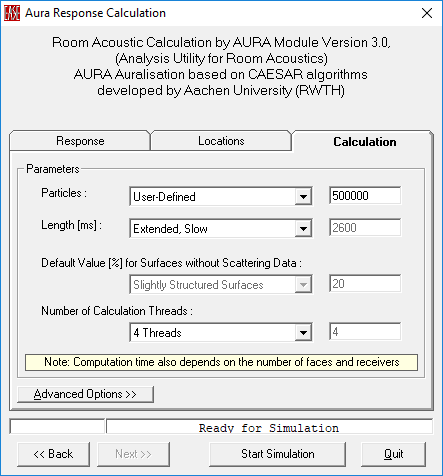
\includegraphics[width=0.95\linewidth]{archivos/capturas/easeopciones1.png}
    \end{subfigure}
    ~ % Añadir el espacio deseado, si se deja la linea en blanco la siguiente subfigura ira en una nueva linea
    \begin{subfigure}[b]{0.47\textwidth}
    	\centering
        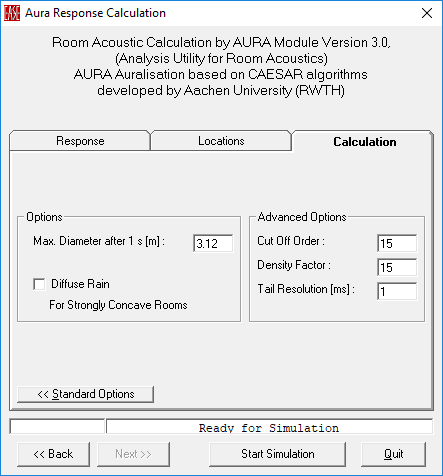
\includegraphics[width=0.95\linewidth]{archivos/capturas/easeopciones2.png}
    \end{subfigure}
    \caption{Ventanas de parámetros para el cálculo de la respuesta al impulso en EASE.}\label{opcionesease}
\end{figure}
\FloatBarrier 


La primera ventana de opciones permite elegir el número de rayos lanzados (\textit{Particles}), pudiendo reducir o aumentar según las necesidades del recinto, también la duración máxima de cada uno de ellos (\textit{Length}) y por último permite seleccionar una dispersión genérica para los materiales que no la tengan definida (no seleccionable si todos los materiales tienen definida la dispersión) y cuántos núcleos de procesador se van a dedicar al cálculo.

En la segunda ventana de opciones, es posible determinar la precisión del campo temprano modificando el diámetro de una esfera imaginaria alrededor del receptor que captará los rayos acústicos (\textit{Max. Diameter after 1s}), a menor valor mayor precisión del campo temprano. Existe la posibilidad de realizar el cálculo con un algoritmo alternativo (\textit{Diffuse rain}) que a grandes rasgos sustituye el cálculo de los rayos dispersos que originalmente son aleatorios para calcular todos los posibles rayos dispersos que impactaran en cada receptor, es útil para recintos donde la forma de estos recintos producen una fuerte focalización del sonido, en este trabajo no se ha hecho uso de este algoritmo. Las tres últimas opciones definen los parámetros de los rayos: a partir de qué número de reflexiones de cada rayo (\textit{Cut Off Order}) se cambia el método de cálculo de \textit{fuente imagen} a trazado de rayos, la densidad de pulsos por milisegundo para la parte tardía (\textit{Density factor}) y la resolución de la cola reverberante (\textit{Tail resolution}).
\\
\par
Los algoritmos utilizados en EASE (\textit{CAESAR}), que no se conocen internamente, devuelven cálculos con altísima densidad de datos que permiten acercarse a los datos de una medida real. La única limitación (solucionado en la futura versión 5, 2019) es la arquitectura de 32 bits y la imposibilidad de utilizar más de 1GB de memoria RAM aunque, como se verá a continuación, es suficiente para obtener buenos resultados.

La historia temporal, obtenida por separado para cada receptor, tiene el siguiente formato una vez exportado a archivo de texto:

\begin{figure}[ht]
    \centering
    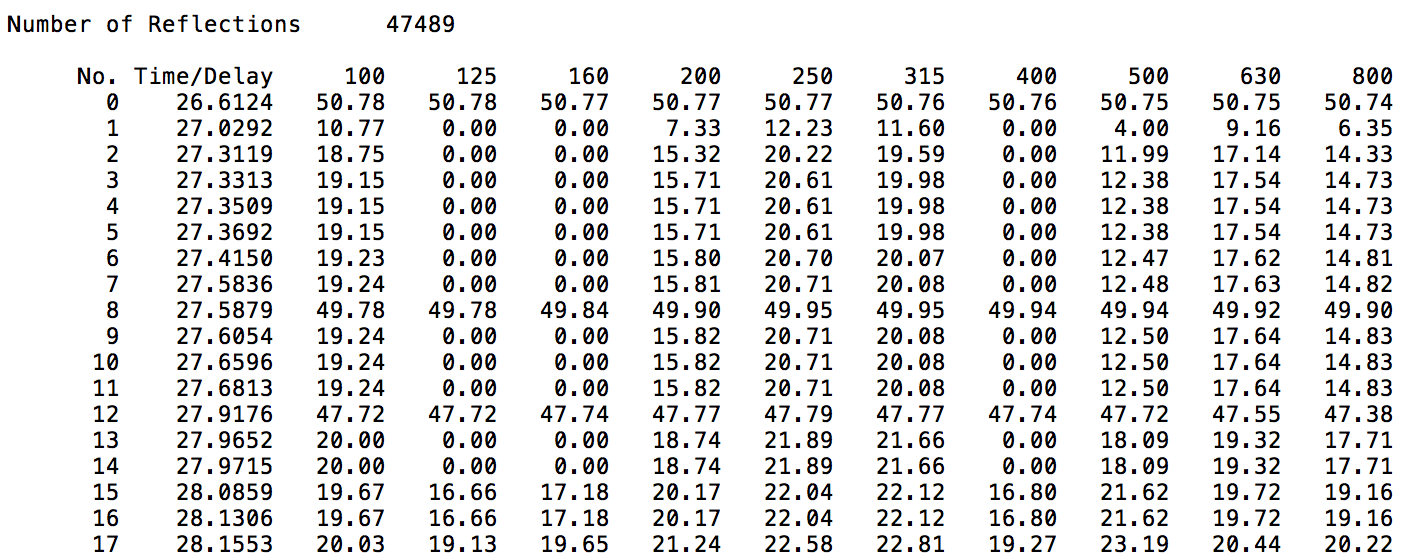
\includegraphics[width=0.8\textwidth]{archivos/capturas/rayeasetxt.png}
    \caption{Porción de la tabla de datos de un receptor generada por el trazado de rayos en EASE.}
\end{figure}
\FloatBarrier

Estos serán finalmente los modelos elegidos para la elaboración del trabajo.

\subsubsection{Aula OP/S003}

Para la simulación del aula OP/S003 en EASE se han ubicado los puntos de recepción en los mismos lugares que en las medidas in situ, 48 receptores para el caso del aula con mobiliario y 24 sin mobiliario, añadiendo 2 receptores para completar el mallado de medida. Las fuentes, una en el centro y otra en la esquina son omnidireccionales con un nivel de presión acústica a 1 metro de 70dB por tercio de octava emitiendo ruido rosa.


El tiempo medio de cálculo ha sido:
\begin{itemize}
\itemsep0em
  \item Con mobiliario: 16 horas.
  \item Sin mobiliario: 2 horas.
\end{itemize}

El modelo tridimensional con mobiliario y sin él se puede observar en la figura \ref{modeloopease}.


\begin{figure}[ht]
    \centering
    \begin{subfigure}[b]{0.45\textwidth}
    	\centering
        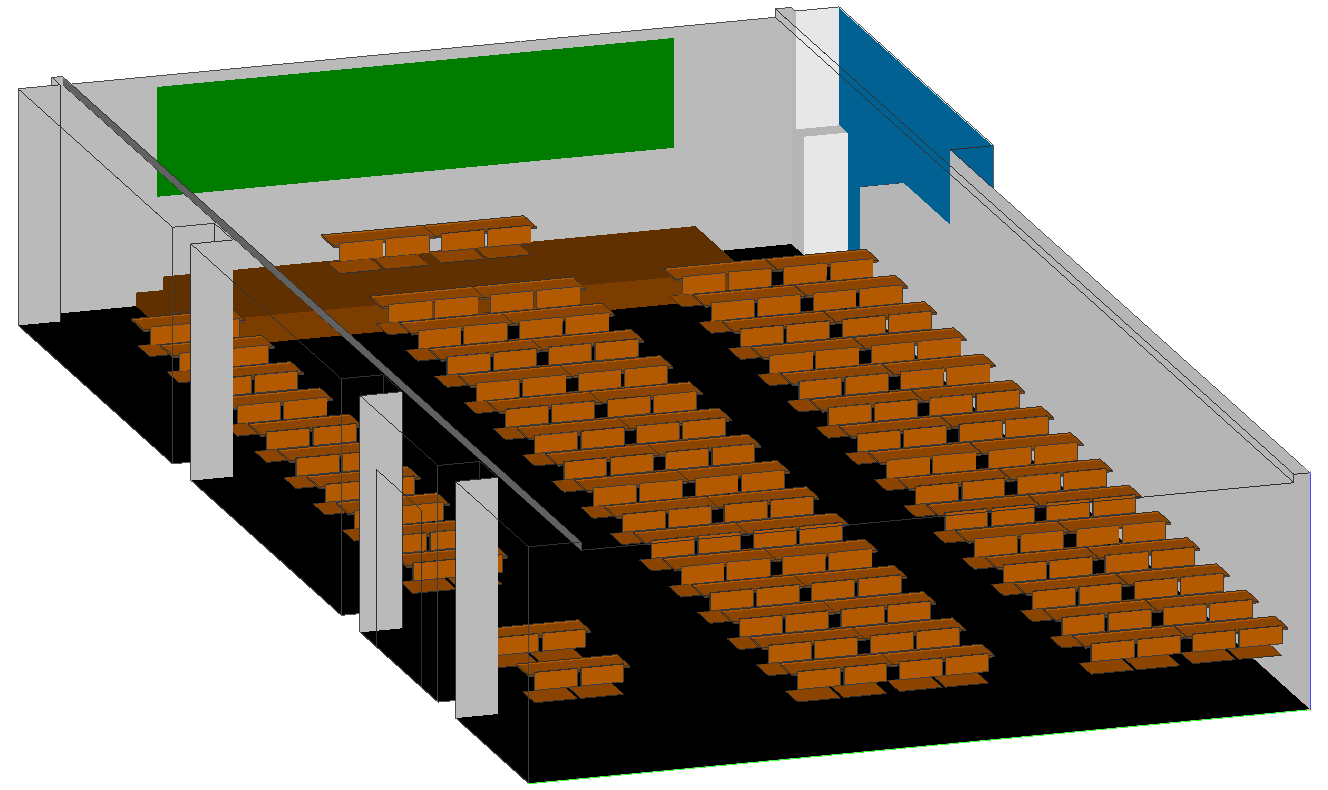
\includegraphics[width=0.9\linewidth]{archivos/capturas/easeopllena.png}
    \end{subfigure}
    ~ % Añadir el espacio deseado, si se deja la linea en blanco la siguiente subfigura ira en una nueva linea
    \begin{subfigure}[b]{0.45\textwidth}
    	\centering
        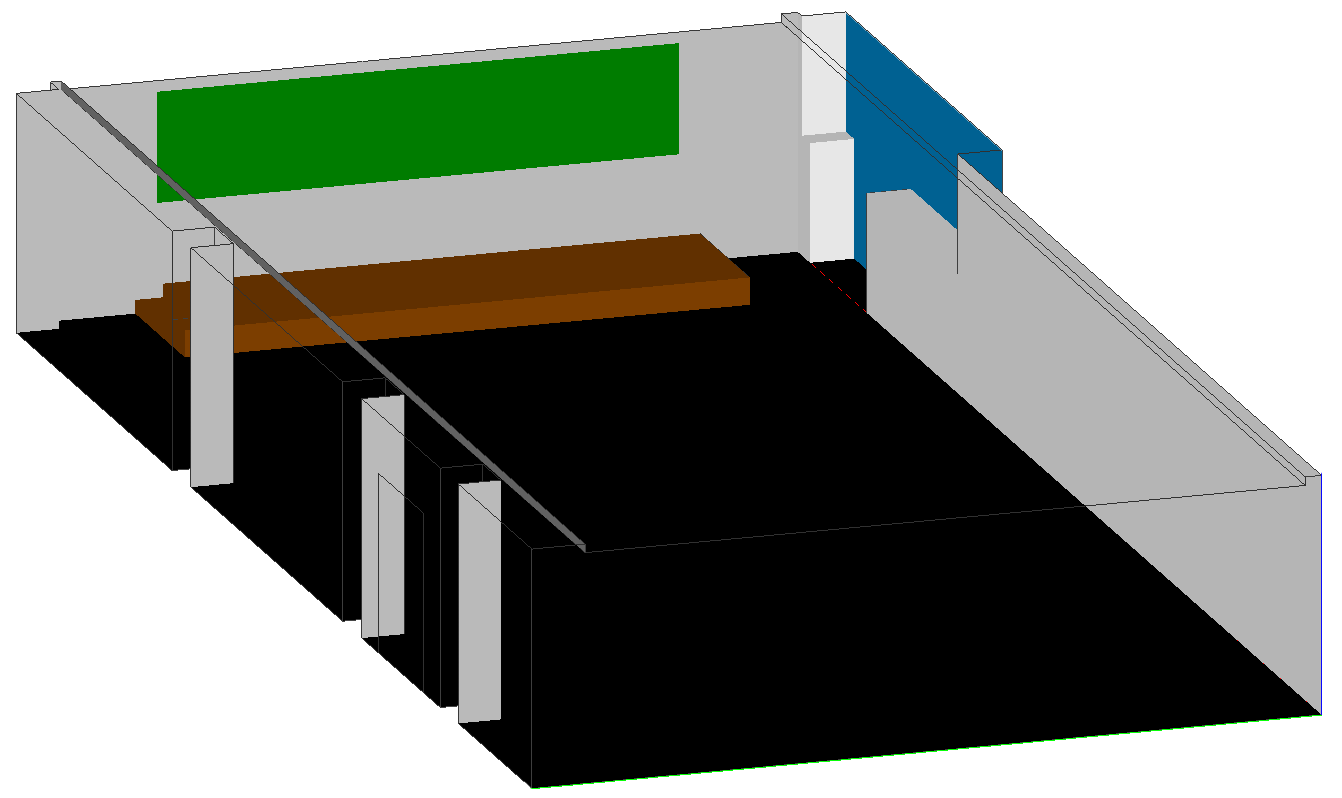
\includegraphics[width=0.9\linewidth]{archivos/capturas/easeopvacia.png}
    \end{subfigure}
    \caption{Modelos del Aula EP/0-26M en EASE.}\label{modeloopease}
\end{figure}
\FloatBarrier 

Los cálculos del tiempo de reverberación por bandas de octava son:

\begin{table}[ht]
\centering
{\scalefont{0.9}
\begin{tabular}{@{}lccccccc@{}}
\toprule
Frecuencia (Hz) & 125 & 250 & 500 & 1000 & 2000 & 4000 & 8000 \\ \midrule
$T30$ Con mobiliario (s) & 1.20 & 1.64 & 1.78 & 1.50 & 1.29 & 1.31 & 1.03 \\
$T30$ Sin mobiliario (s) & 1.19 & 1.84 & 1.98 & 1.84 & 1.65 & 1.68 & 1.30 \\ \bottomrule
\end{tabular}
}
\caption{Tiempos de reverberación calculados en el aula OP/S003 por banda de octava, con y sin mobiliario mediante EASE (T30 extrapolado).}
\label{tab:revopease}
\end{table}
\FloatBarrier

Comparando con las medidas in situ se obtiene la desviación entre los resultados:

\begin{table}[ht]
\centering
{\scalefont{0.9}
\begin{tabular}{@{}lccccccc@{}}
\toprule
Frecuencia (Hz) & 125 & 250 & 500 & 1000 & 2000 & 4000 & 8000 \\ \midrule
$\sigma_{T30}$ Con mobiliario (s) & 0.06 & 0.06 & 0.04 & 0.05 & 0.03 & 0.04 & 0.01 \\
$\sigma_{T30}$ Sin mobiliario (s) & 0.01 & 0.02 & 0.04 & 0.02 & 0.03 & 0.01 & 0.00 \\ \bottomrule
\end{tabular}
}
\caption{Desviación de los tiempos de reverberación calculados en el aula OP/S003 por banda de octava, con y sin mobiliario mediante EASE (T30 extrapolado) respecto a los medidos in situ.}
\label{tab:desrevopease}
\end{table}
\FloatBarrier

Las curvas de los campos acústicos obtenidos se muestran junto a las obtenidas in situ (corrigiendo los niveles de las curvas in situ) en las figuras \ref{graf:easeopmob} y \ref{graf:easeopnomob}.

\begin{figure}[ht]
    \begin{subfigure}[b]{0.4\textwidth}
    	\centering%
         {\scalefont{0.8}%
    %%%%%%%%%%%%%%%%%%%%%%%%%%%%%%%%%%%%%%%%%%%%%%%%%%%%%%%%%%%%%%%%%%%%%%%%
% Escuela Politécnica Superior de la Universidad de Alicante
% Realizado por: Jose Manuel Requena Plens
% Contacto: info@jmrplens.com / Telegram:@jmrplens
%%%%%%%%%%%%%%%%%%%%%%%%%%%%%%%%%%%%%%%%%%%%%%%%%%%%%%%%%%%%%%%%%%%%%%%%

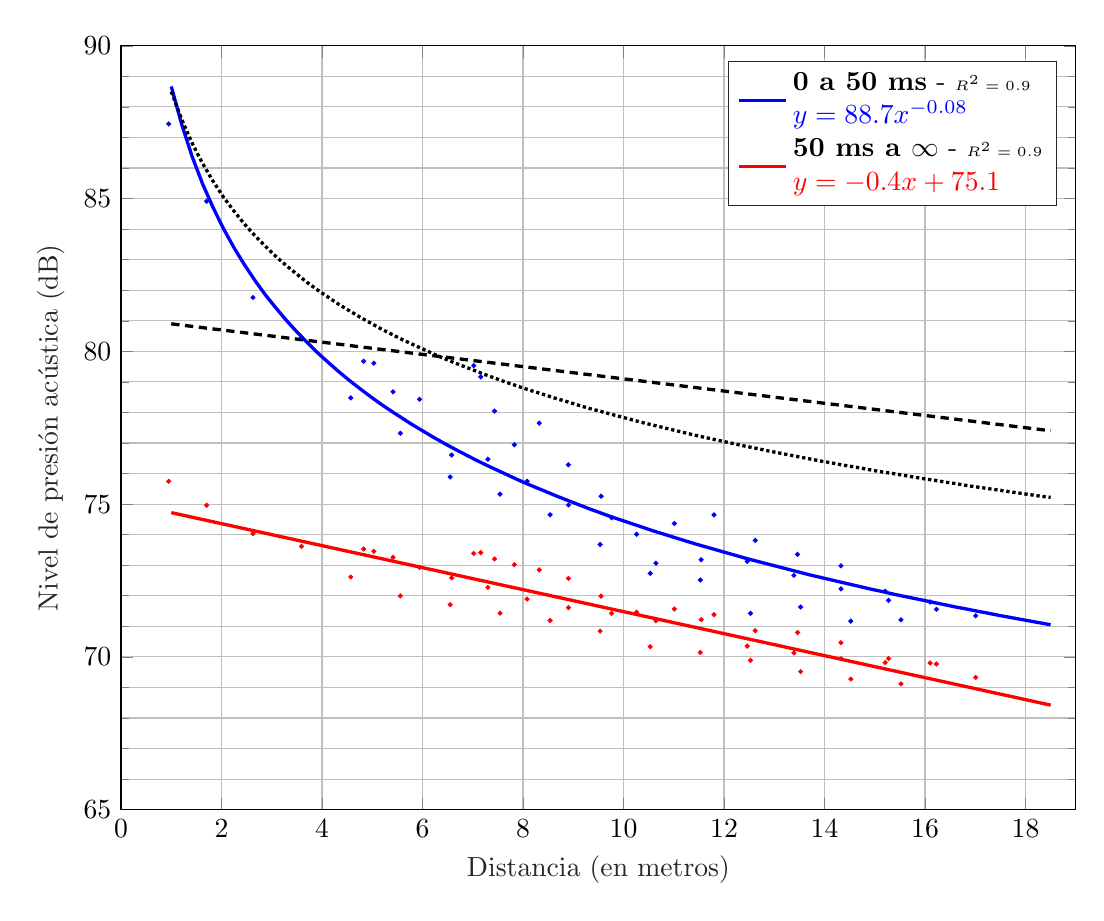
\begin{tikzpicture}

\begin{axis}[%
width=\textwidth,
height=0.8\textwidth,
at={(0\textwidth,0\textwidth)},
scale only axis,
xmin=0,
xmax=19,
xlabel style={font=\color{white!15!black}},
xlabel={Distancia (en metros)},
ymin=65,
ymax=90,
ylabel style={font=\color{white!15!black}},
ylabel={Nivel de presión acústica (dB)},
axis background/.style={fill=white},
xmajorgrids,
xminorgrids,
ymajorgrids,
yminorgrids,
minor y tick num= 4,
legend style={legend cell align=left, align=left, draw=white!15!black}
]
% Curvas CATT
\addplot[color=blue,domain=1:18.5, samples=85,line width=1.2]{88.67*x^(-0.076)};
\addlegendentry{\textbf{0 a 50 ms} - \tiny{$R^2 = 0.9$}\\$\color{blue}y = 88.7·x^{-0.08}$}

\addplot[color=red,domain=1:18.5, samples=85,line width=1.2]{-0.36*x+75.08};
\addlegendentry{\textbf{50 ms a $\infty$} - \tiny{$R^2 = 0.9$}\\$\color{red}y = -0.4·x+75.1$}

% Curvas insitu
\addplot[color=black,densely dotted,line width=1.2pt,domain=1:18.5, samples=85]{82.8*x^(-0.06)+5.7};
\addplot[color=black,densely dashed,line width=1.2pt,domain=1:18.5, samples=85]{-0.2*x+75.4+5.7};

% Puntos
\addplot [color=blue, only marks,mark size=0.7pt]
  table[row sep=crcr]{%
0.948683298050514	87.4420961737289\\
1.70293863659264	84.9101891335025\\
2.62678510731274	81.7616782663821\\
3.59165699921359	80.4594949830013\\
4.57165178026498	78.4743406612998\\
4.82700735445887	79.6749357146687\\
5.02991053598372	79.6099301559067\\
5.41294744108974	78.6769987882943\\
5.55877684387492	77.3163745316826\\
5.94138031100518	78.4288425873064\\
6.54980915752513	75.8895421602869\\
6.58027355054484	76.6065679800343\\
7.01854685814663	79.5332904135811\\
7.15960892786750	79.1637036731850\\
7.30068489937759	76.4696786318159\\
7.43370701601832	78.0426918821762\\
7.54320886625844	75.3265970040634\\
7.82687677173980	76.9431242903696\\
8.08084154033477	75.7470760371774\\
8.32225930862527	77.6515180556227\\
8.53814968245463	74.6503337666187\\
8.90280854562199	76.2882001100458\\
8.90505474435727	74.9696918747926\\
9.53414914924242	73.6779688290171\\
9.55300999685439	75.2562900009924\\
9.76217188949263	74.5542057113502\\
10.2596296229445	74.0139270404374\\
10.5309068935206	72.7337213913187\\
10.6442472725881	73.0676630652864\\
11.0118118400198	74.3643239413052\\
11.5282262295637	72.5156670594346\\
11.5455619178973	73.1790230553865\\
11.8008474271978	74.6480877242953\\
12.4619420637395	73.1237773193099\\
12.5259730160974	71.4238616260825\\
12.6198256723300	73.8124835540362\\
13.3902949930164	72.6668164377848\\
13.4632834033901	73.3553088248711\\
13.5240526470433	71.6308006342674\\
14.3268977800499	72.9812532742246\\
14.3282936876657	72.2246594069741\\
14.5223964964464	71.1682136571806\\
15.2072351201657	72.1472482510490\\
15.2741611880980	71.8490374455435\\
15.5209535789526	71.2130961699322\\
16.1015527201571	71.7972079304157\\
16.2265215003093	71.5564158086635\\
17.0076453396700	71.3434463853828\\
};

\addplot [color=red, only marks,mark size=0.7pt]
  table[row sep=crcr]{%
0.948683298050514	75.7466093611256\\
1.70293863659264	74.9620670277384\\
2.62678510731274	74.0349450671551\\
3.59165699921359	73.6136355964006\\
4.57165178026498	72.6143242927786\\
4.82700735445887	73.5297411201215\\
5.02991053598372	73.4545810943120\\
5.41294744108974	73.2570047547895\\
5.55877684387492	71.9953320089908\\
5.94138031100518	72.9261908308415\\
6.54980915752513	71.7082447243117\\
6.58027355054484	72.5836610994912\\
7.01854685814663	73.3840340464182\\
7.15960892786750	73.4107069259186\\
7.30068489937759	72.2746394429866\\
7.43370701601832	73.2059014915045\\
7.54320886625844	71.4306024661113\\
7.82687677173980	73.0164487523306\\
8.08084154033477	71.8905323647189\\
8.32225930862527	72.8454946686892\\
8.53814968245463	71.1902311018161\\
8.90280854562199	72.5680465538569\\
8.90505474435727	71.6086258572677\\
9.53414914924242	70.8424605573549\\
9.55300999685439	71.9872749381950\\
9.76217188949263	71.4243003629265\\
10.2596296229445	71.4626874668587\\
10.5309068935206	70.3312921929216\\
10.6442472725881	71.1783143298641\\
11.0118118400198	71.5645996978242\\
11.5282262295637	70.1457115471035\\
11.5455619178973	71.2196441725215\\
11.8008474271978	71.3841618108768\\
12.4619420637395	70.3540383167020\\
12.5259730160974	69.8865691165710\\
12.6198256723300	70.8567389463696\\
13.3902949930164	70.1294840170384\\
13.4632834033901	70.7974414700959\\
13.5240526470433	69.5163505183946\\
14.3268977800499	70.4633816579043\\
14.3282936876657	69.9382170961490\\
14.5223964964464	69.2742569517347\\
15.2072351201657	69.8137378666177\\
15.2741611880980	69.9434230397247\\
15.5209535789526	69.1147710489021\\
16.1015527201571	69.7997558140489\\
16.2265215003093	69.7662404816367\\
17.0076453396700	69.3266560212886\\
  };
\end{axis}
\end{tikzpicture}%%
    }
    \caption{Fuente en la esquina}%
    \end{subfigure}%
    \hspace{1.9cm}%
    \begin{subfigure}[b]{0.4\textwidth}%
    	\centering%
        {\scalefont{0.8}%
    %%%%%%%%%%%%%%%%%%%%%%%%%%%%%%%%%%%%%%%%%%%%%%%%%%%%%%%%%%%%%%%%%%%%%%%%
% Escuela Politécnica Superior de la Universidad de Alicante
% Realizado por: Jose Manuel Requena Plens
% Contacto: info@jmrplens.com / Telegram:@jmrplens
%%%%%%%%%%%%%%%%%%%%%%%%%%%%%%%%%%%%%%%%%%%%%%%%%%%%%%%%%%%%%%%%%%%%%%%%

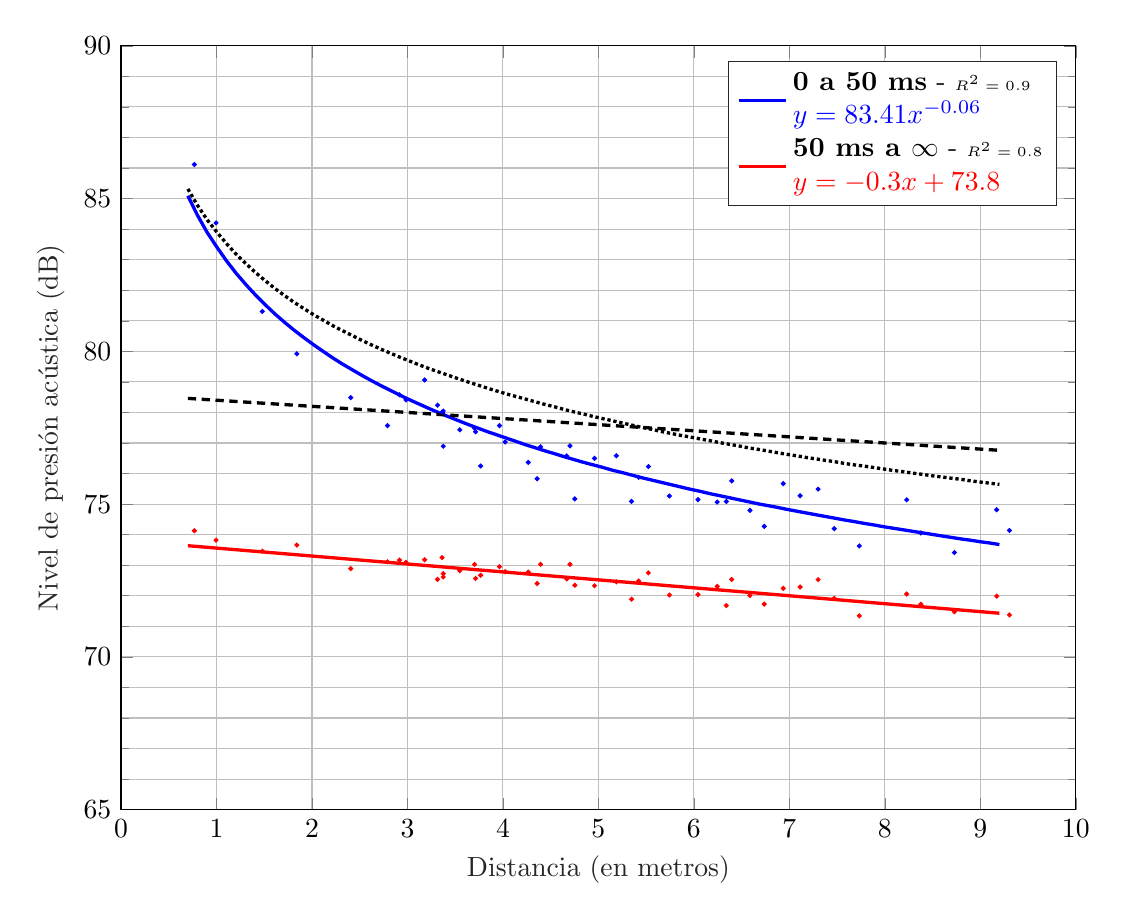
\begin{tikzpicture}

\begin{axis}[%
width=\textwidth,
height=0.8\textwidth,
at={(0\textwidth,0\textwidth)},
scale only axis,
xmin=0,
xmax=10,
xlabel style={font=\color{white!15!black}},
xlabel={Distancia (en metros)},
ymin=65,
ymax=90,
ylabel style={font=\color{white!15!black}},
ylabel={Nivel de presión acústica (dB)},
axis background/.style={fill=white},
xmajorgrids,
xminorgrids,
ymajorgrids,
yminorgrids,
minor y tick num= 4,
legend style={legend cell align=left, align=left, draw=white!15!black}
]
% Curvas CATT
\addplot[color=blue,domain=0.7:9.2, samples=85,line width=1.2]{83.41*x^(-0.056)};
\addlegendentry{\textbf{0 a 50 ms} - \tiny{$R^2 = 0.9$}\\$\color{blue}y = 83.41·x^{-0.06}$}

\addplot[color=red,domain=0.7:9.2, samples=85,line width=1.2]{-0.26*x+73.82};
\addlegendentry{\textbf{50 ms a $\infty$} - \tiny{$R^2 = 0.8$}\\$\color{red}y = -0.3·x+73.8$}

% Curvas in situ
\addplot[color=black,densely dotted,line width=1.2pt,domain=0.7:9.2, samples=85]{78.7*x^(-0.05)+5.2};
\addplot[color=black,densely dashed,line width=1.2pt,domain=0.7:9.2, samples=85]{-0.2*x+73.40+5.2};

% Puntos
\addplot [color=blue, only marks,mark size=0.7pt]
  table[row sep=crcr]{%
0.768114574786861	86.1151209834186\\
0.994987437106620	84.2006220749183\\
1.47986485869488	81.3061497374244\\
1.84119526395220	79.9195372037548\\
2.40624188310319	78.4865600582681\\
2.79105714739057	77.5693313701104\\
2.91719042916296	78.5775710498257\\
2.98496231131986	78.4132992519398\\
3.17962261911693	79.0635332588934\\
3.31511689085016	78.2372943258897\\
3.36303434416005	78.0042986008184\\
3.37490740613724	78.0459892730732\\
3.37490740613724	76.8927880546138\\
3.54823899984204	77.4307367057662\\
3.70270171631472	77.4800244755223\\
3.71348892552543	77.3645059391775\\
3.76696164036747	76.2459719606801\\
3.96358423652128	77.5681487439912\\
4.02367990774614	77.0323472348671\\
4.26497362242723	76.3648237256779\\
4.35775171390019	75.8284411884799\\
4.39431450854397	76.8732348291037\\
4.66797600679352	76.5757147611622\\
4.70212717820350	76.9052972256966\\
4.75289385532646	75.1700494276000\\
4.95883050728698	76.4977402620397\\
5.18748493973718	76.5821252214208\\
5.34696175411794	75.0887889213815\\
5.42125446737192	75.8744120398807\\
5.52358579185659	76.2279962709424\\
5.74369219230975	75.2647467994662\\
6.04235053600832	75.1464316139994\\
6.24419730629967	75.0670281524809\\
6.33955834423819	75.0843761003440\\
6.39609255717895	75.7606600082998\\
6.58710862214978	74.7936453163927\\
6.73721010508059	74.2695736535206\\
6.93613725354394	75.6713115261933\\
7.11266476083331	75.2753784620270\\
7.30136973450872	75.4903430239852\\
7.46927037936103	74.1973192043746\\
7.73239936888932	73.6294515206552\\
8.22860863086828	75.1401887466692\\
8.37794724261260	74.0549074528739\\
8.72868833216080	73.4131544969651\\
9.17115041856800	74.8155560158274\\
9.30537479094743	74.1360934824533\\
  };
  
  \addplot [color=red, only marks,mark size=0.7pt]
  table[row sep=crcr]{%
0.768114574786861	74.1295976540934\\
0.994987437106620	73.8177138103166\\
1.47986485869488	73.4589181148590\\
1.84119526395220	73.6598086186530\\
2.40624188310319	72.8867825488117\\
2.79105714739057	73.1135521351630\\
2.91719042916296	73.1647629514726\\
2.98496231131986	73.0916307674029\\
3.17962261911693	73.1803431221767\\
3.31511689085016	72.5344467335989\\
3.36303434416005	73.2488027002141\\
3.37490740613724	72.6139473999912\\
3.37490740613724	72.7219307647258\\
3.54823899984204	72.8190228790923\\
3.70270171631472	73.0241831128930\\
3.71348892552543	72.5676515469103\\
3.76696164036747	72.6703938335031\\
3.96358423652128	72.9514345811682\\
4.02367990774614	72.7892478260028\\
4.26497362242723	72.7742009221803\\
4.35775171390019	72.3995092556766\\
4.39431450854397	73.0284244764012\\
4.66797600679352	72.5526319108744\\
4.70212717820350	73.0254128565198\\
4.75289385532646	72.3446387253937\\
4.95883050728698	72.3275338645387\\
5.18748493973718	72.4558840373747\\
5.34696175411794	71.8863187877500\\
5.42125446737192	72.4800337339836\\
5.52358579185659	72.7485583462402\\
5.74369219230975	72.0219555216252\\
6.04235053600832	72.0366771610408\\
6.24419730629967	72.3070336513729\\
6.33955834423819	71.6797739630234\\
6.39609255717895	72.5329165819127\\
6.58710862214978	72.0075013249338\\
6.73721010508059	71.7267835510540\\
6.93613725354394	72.2419569679648\\
7.11266476083331	72.2855033912216\\
7.30136973450872	72.5277244326909\\
7.46927037936103	71.9140168012540\\
7.73239936888932	71.3434241258055\\
8.22860863086828	72.0559415345805\\
8.37794724261260	71.7212915321893\\
8.72868833216080	71.4779938637759\\
9.17115041856800	71.9860666960003\\
9.30537479094743	71.3718349358966\\
  };
\end{axis}
\end{tikzpicture}%%
    }
    \caption{Fuente en el centro}%
    \end{subfigure}
    \caption{Campos acústicos en el aula OP/S003 con mobiliario simulado en EASE. Se muestran las curvas in situ (negro) con el nivel global modificado para poder comparar.}
    \label{graf:easeopmob}%
\end{figure}
\FloatBarrier 


\begin{figure}[ht]
    \begin{subfigure}[b]{0.4\textwidth}
    	\centering%
         {\scalefont{0.8}%
    %%%%%%%%%%%%%%%%%%%%%%%%%%%%%%%%%%%%%%%%%%%%%%%%%%%%%%%%%%%%%%%%%%%%%%%%
% Escuela Politécnica Superior de la Universidad de Alicante
% Realizado por: Jose Manuel Requena Plens
% Contacto: info@jmrplens.com / Telegram:@jmrplens
%%%%%%%%%%%%%%%%%%%%%%%%%%%%%%%%%%%%%%%%%%%%%%%%%%%%%%%%%%%%%%%%%%%%%%%%

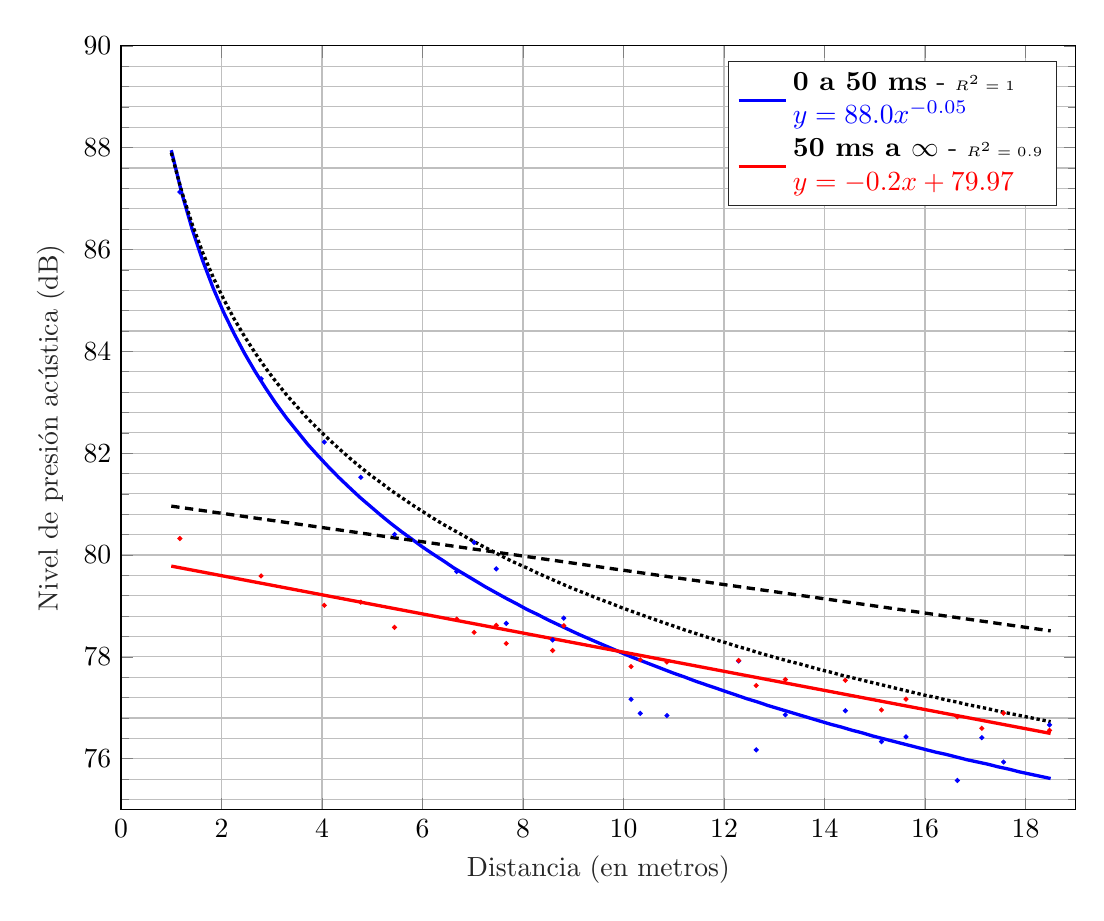
\begin{tikzpicture}

\begin{axis}[%
width=\textwidth,
height=0.8\textwidth,
at={(0\textwidth,0\textwidth)},
scale only axis,
xmin=0,
xmax=19,
xlabel style={font=\color{white!15!black}},
xlabel={Distancia (en metros)},
ymin=75,
ymax=90,
ylabel style={font=\color{white!15!black}},
ylabel={Nivel de presión acústica (dB)},
axis background/.style={fill=white},
xmajorgrids,
xminorgrids,
ymajorgrids,
yminorgrids,
minor y tick num= 4,
legend style={legend cell align=left, align=left, draw=white!15!black}
]
% Curvas EASE
\addplot[color=blue,domain=1:18.5, samples=85,line width=1.2]{87.95*x^(-0.05187)};
\addlegendentry{\textbf{0 a 50 ms} - \tiny{$R^2 = 1$}\\$\color{blue}y = 88.0·x^{-0.05}$}

\addplot[color=red,domain=1:18.5, samples=85,line width=1.2]{-0.1878*x+79.97};
\addlegendentry{\textbf{50 ms a $\infty$} - \tiny{$R^2 = 0.9$}\\$\color{red}y = -0.2·x+79.97$}

% Errores
%\addplot[color=blue, only marks,,mark size=0.7pt,mark=o,error bars/.cd,y dir=both, y explicit] 
%		table [x=x,y=y, y error plus=ymas, y error minus=ymenos]
%			{archivos/graficastikz/UtilErrores.dat};
			
%\addplot[color=red, only marks,mark=o,error bars/.cd,y dir=both, y explicit] 
%		table [x=x,y=y, y error plus=ymas, y error minus=ymenos]
%			{archivos/graficastikz/PerjudicialErrores.dat};


% Curvas insitu
\addplot[color=black,densely dotted,line width=1.2pt,domain=1:18.5, samples=85]{82.4*x^(-0.05)+5.5};
\addplot[color=black,densely dashed,line width=1.2pt,domain=1:18.5, samples=85]{-0.14*x+75.6+5.5};


% Puntos
\addplot [color=blue, only marks,mark size=0.7pt]
  table[row sep=crcr]{%
1.17046999107196	87.1277550611968\\
2.78747197295327	83.4623086675921\\
4.04598566482878	82.2179401358662\\
4.77179211617606	81.5257517559293\\
5.44357419348722	80.4045039689526\\
6.68075594525051	79.6754872626557\\
7.02637886823647	80.2469029713596\\
7.46793144049944	79.7283523968088\\
7.66615940350838	78.6559229050811\\
8.58894638474359	78.3326673816969\\
8.81093071133805	78.7617201801592\\
10.1498768465435	77.1663192028700\\
10.3329569823938	76.8891694043067\\
10.8637010268140	76.8468643393087\\
12.2890194889584	77.9181962233661\\
12.6400158227749	76.1735762643118\\
13.2200605142337	76.8612684404271\\
14.4142290810157	76.9428881306448\\
15.1334067545943	76.3340029077443\\
15.6211395230950	76.4290703842402\\
16.6439178080162	75.5728813031650\\
17.1295067062657	76.4126252632454\\
17.5618905588208	75.9345334655598\\
18.4775539506722	76.6630383745993\\
};

\addplot [color=red, only marks,mark size=0.7pt]
  table[row sep=crcr]{%
1.17046999107196	80.3231940709341\\
2.78747197295327	79.5902397011391\\
4.04598566482878	79.0120257322755\\
4.77179211617606	79.0732056591827\\
5.44357419348722	78.5794103477747\\
6.68075594525051	78.7408951295518\\
7.02637886823647	78.4806520089487\\
7.46793144049944	78.6186486954362\\
7.66615940350838	78.2622920553155\\
8.58894638474359	78.1230323668705\\
8.81093071133805	78.6111774265353\\
10.1498768465435	77.8093052083963\\
10.3329569823938	77.9430570409649\\
10.8637010268140	77.8977458350415\\
12.2890194889584	77.9283000590244\\
12.6400158227749	77.4366536941934\\
13.2200605142337	77.5555167518319\\
14.4142290810157	77.5382759101964\\
15.1334067545943	76.9569768837744\\
15.6211395230950	77.1695938485288\\
16.6439178080162	76.8237758577911\\
17.1295067062657	76.5974351112101\\
17.5618905588208	76.8959648117646\\
18.4775539506722	76.5579088024192\\
  };
\end{axis}
\end{tikzpicture}%%
    }
    \caption{Fuente en la esquina}%
    \end{subfigure}%
    \hspace{1.9cm}%
    \begin{subfigure}[b]{0.4\textwidth}%
    	\centering%
        {\scalefont{0.8}%
    %%%%%%%%%%%%%%%%%%%%%%%%%%%%%%%%%%%%%%%%%%%%%%%%%%%%%%%%%%%%%%%%%%%%%%%%
% Escuela Politécnica Superior de la Universidad de Alicante
% Realizado por: Jose Manuel Requena Plens
% Contacto: info@jmrplens.com / Telegram:@jmrplens
%%%%%%%%%%%%%%%%%%%%%%%%%%%%%%%%%%%%%%%%%%%%%%%%%%%%%%%%%%%%%%%%%%%%%%%%

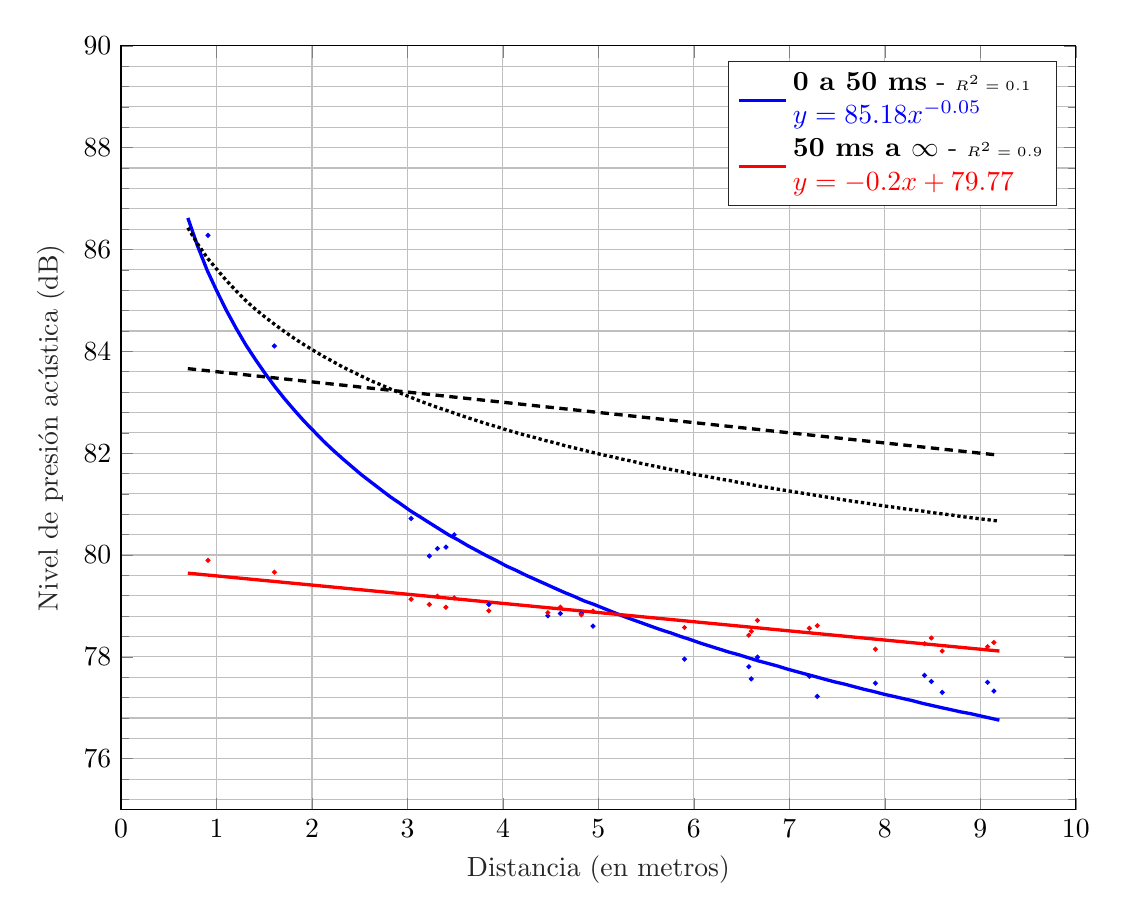
\begin{tikzpicture}

\begin{axis}[%
width=\textwidth,
height=0.8\textwidth,
at={(0\textwidth,0\textwidth)},
scale only axis,
xmin=0,
xmax=10,
xlabel style={font=\color{white!15!black}},
xlabel={Distancia (en metros)},
ymin=75,
ymax=90,
ylabel style={font=\color{white!15!black}},
ylabel={Nivel de presión acústica (dB)},
axis background/.style={fill=white},
xmajorgrids,
xminorgrids,
ymajorgrids,
yminorgrids,
minor y tick num= 4,
legend style={legend cell align=left, align=left, draw=white!15!black}
]
% Curvas EASE
\addplot[color=blue,domain=0.7:9.2, samples=85,line width=1.2]{85.18*x^(-0.047)};
\addlegendentry{\textbf{0 a 50 ms} - \tiny{$R^2 = 0.1$}\\$\color{blue}y = 85.18·x^{-0.05}$}

\addplot[color=red,domain=0.7:9.2, samples=85,line width=1.2]{-0.18*x+79.77};
\addlegendentry{\textbf{50 ms a $\infty$} - \tiny{$R^2 = 0.9$}\\$\color{red}y = -0.2·x+79.77$}

% Curvas in situ
\addplot[color=black,densely dotted,line width=1.2pt,domain=0.7:9.2, samples=85]{76.9*x^(-0.03)+8.7};
\addplot[color=black,densely dashed,line width=1.2pt,domain=0.7:9.2, samples=85]{-0.2*x+75.1+8.7};

% Puntos
\addplot [color=blue, only marks,mark size=0.7pt]
  table[row sep=crcr]{%
 0.911043357914430	86.2772796781886\\
1.60623784042090	84.1056446478500\\
3.03809150619266	80.7162943773909\\
3.22955105239103	79.9791235432895\\
3.31360830515618	80.1257164588809\\
3.40293990543471	80.1549543981309\\
3.48998567332303	80.3976116923752\\
3.85259652701915	79.0293836816767\\
4.46989932772540	78.8058727354038\\
4.60217339960154	78.8512802176443\\
4.82104760399646	78.8496625245368\\
4.94393567919325	78.6032259795649\\
5.90169467187180	77.9558802268358\\
6.57495247131110	77.8065806803430\\
6.60151497763960	77.5670065559296\\
6.66558324529819	77.9950758659912\\
7.20971566707037	77.6179645821617\\
7.29246186140181	77.2229572843838\\
7.90126572138920	77.4832543472834\\
8.41605608346332	77.6356061014582\\
8.48704895708750	77.5171417313596\\
8.60116271209887	77.3035533865362\\
9.07634287585038	77.4993226551940\\
9.14220979851152	77.3278313594281\\
  };
  
  \addplot [color=red, only marks,mark size=0.7pt]
  table[row sep=crcr]{%
0.911043357914430	79.8951008237853\\
1.60623784042090	79.6634802579777\\
3.03809150619266	79.1311060267053\\
3.22955105239103	79.0290689238144\\
3.31360830515618	79.1915465704714\\
3.40293990543471	78.9738863429516\\
3.48998567332303	79.1574260253045\\
3.85259652701915	78.9034083062506\\
4.46989932772540	78.8673915409159\\
4.60217339960154	78.9747462523916\\
4.82104760399646	78.8249463712323\\
4.94393567919325	78.8986754815038\\
5.90169467187180	78.5761350266222\\
6.57495247131110	78.4254000607376\\
6.60151497763960	78.5015455533187\\
6.66558324529819	78.7147432854439\\
7.20971566707037	78.5621450983992\\
7.29246186140181	78.6112877631831\\
7.90126572138920	78.1512018038794\\
8.41605608346332	78.2574617650506\\
8.48704895708750	78.3698657405733\\
8.60116271209887	78.1141880570530\\
9.07634287585038	78.2003228792576\\
9.14220979851152	78.2818430326449\\
  };
\end{axis}
\end{tikzpicture}%%
    }
    \caption{Fuente en el centro}%
    \end{subfigure}
    \caption{Campos acústicos en el aula OP/S003 sin mobiliario simulado en EASE. Se muestran las curvas in situ (negro) con el nivel global modificado para poder comparar.}
    \label{graf:easeopnomob}%
\end{figure}
\FloatBarrier 

Los resultados con mobiliario tienen los mismos problemas observados en CATT-Acoustic, el hecho de introducir un gran número de planos (mobiliario) produce que la mayoría de los rayos reflejados se eliminen antes de alcanzar un receptor, reduciendo la densidad de datos resultante y por tanto obteniendo menor energía, sobretodo en el campo perjudicial.

En el caso sin mobiliario con fuente en la esquina es muy similar a los resultados obtenidos en las medidas in situ, aunque con la fuente en el centro la energía es mucho menor.

\subsubsection{Aula EP/0-26M}

Para la simulación del aula EP/0-26M en EASE se han ubicado los puntos de recepción en los mismos lugares que en las medidas in situ, 30 receptores. Las fuentes, una en el centro y otra en la esquina son omnidireccionales con un nivel de presión acústica a 1 metro de 70dB por tercio de octava emitiendo ruido rosa.

El tiempo medio de cálculo ha sido:
\begin{itemize}
\itemsep0em
  \item Con mobiliario: 4 horas.
  \item Sin mobiliario: 2 horas.
\end{itemize}



El modelo tridimensional con mobiliario y sin él se puede observar en la figura \ref{modeloepsease}.

\begin{figure}[ht]
    \centering
    \begin{subfigure}[b]{0.45\textwidth}
    	\centering
        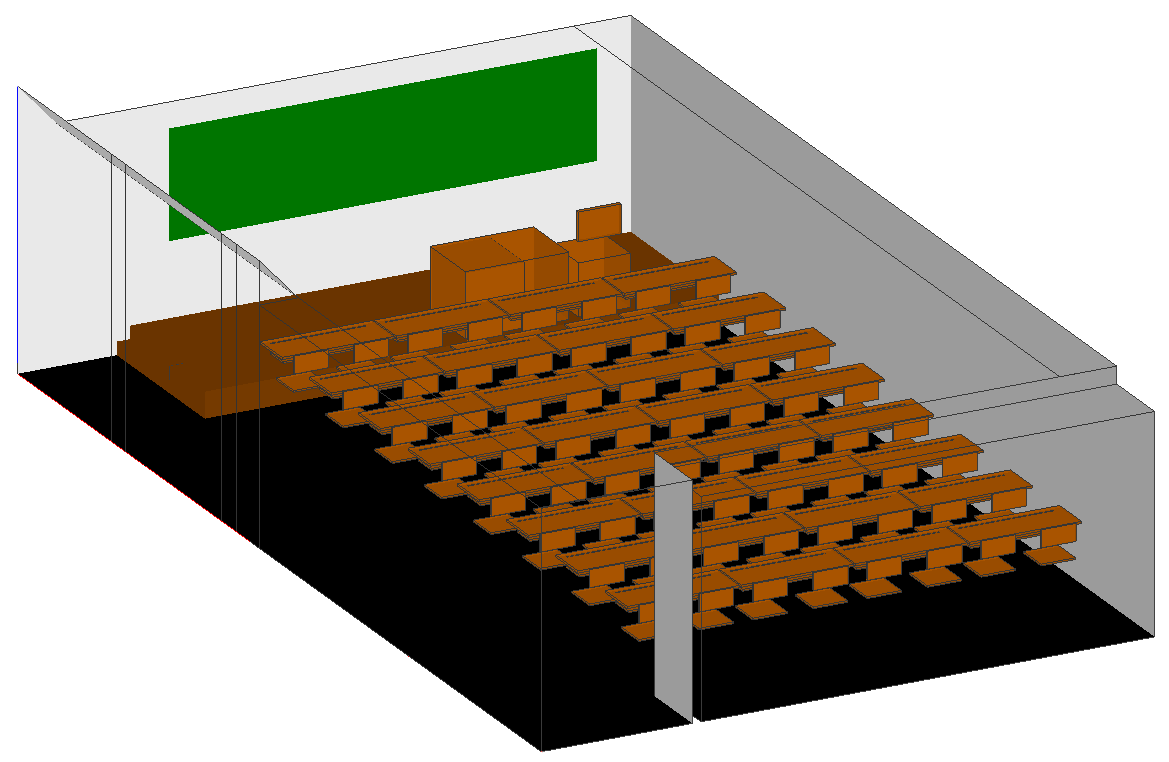
\includegraphics[width=0.9\linewidth]{archivos/capturas/easeepsllena.png}
    \end{subfigure}
    ~ % Añadir el espacio deseado, si se deja la linea en blanco la siguiente subfigura ira en una nueva linea
    \begin{subfigure}[b]{0.45\textwidth}
    	\centering
        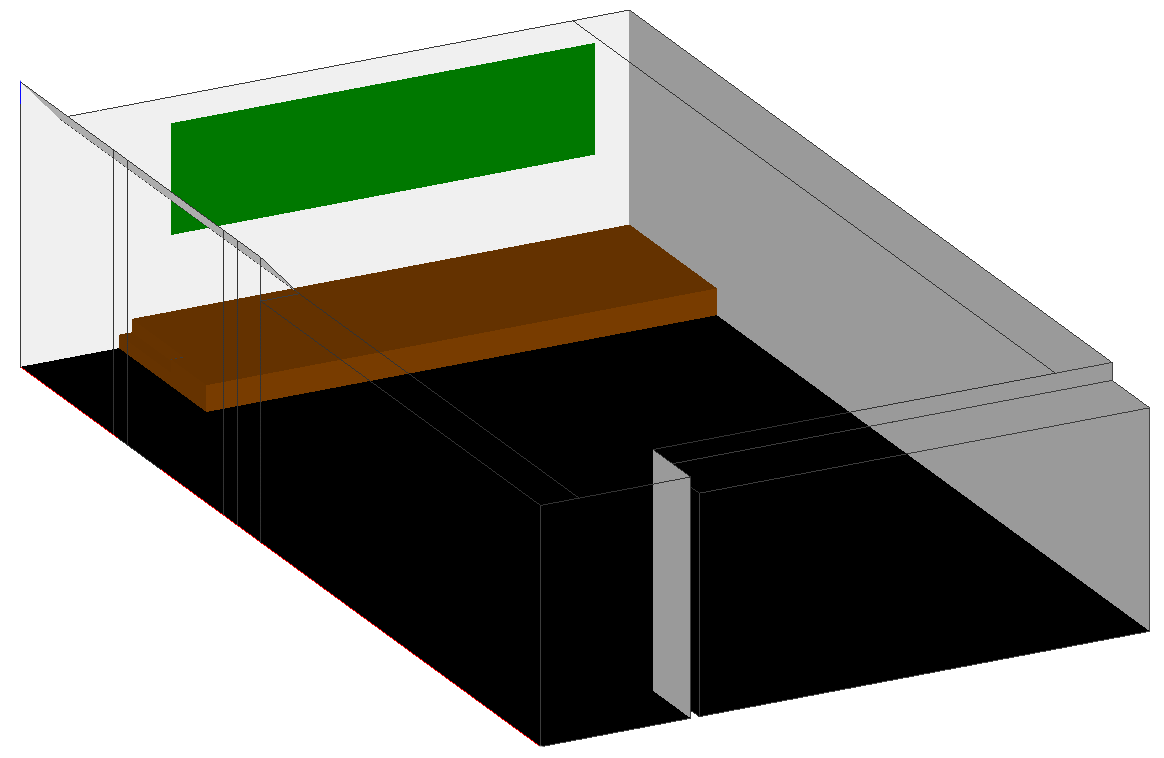
\includegraphics[width=0.9\linewidth]{archivos/capturas/easeepsvacia.png}
    \end{subfigure}
    \caption{Modelos del Aula EP/0-26M en EASE.}\label{modeloepsease}
\end{figure}
\FloatBarrier 


Los cálculos del tiempo de reverberación por bandas de octava son:

\begin{table}[ht]
\centering
{\scalefont{0.9}
\begin{tabular}{@{}lccccccc@{}}
\toprule
Frecuencia (Hz) & 125 & 250 & 500 & 1000 & 2000 & 4000 & 8000 \\ \midrule
$T30$ Con mobiliario (s) & 1.25 & 1.35 & 1.42 & 1.32 & 1.09 & 0.95 & 0.82 \\
$T30$ Sin mobiliario (s) & 1.35 & 1.59 & 1.57 & 1.45 & 1.32 & 1.16 & 0.84 \\ \bottomrule
\end{tabular}
}
\caption{Tiempos de reverberación calculados en el aula EP/0-26M por banda de octava, con y sin mobiliario mediante EASE (T30 extrapolado).}
\label{tab:revepsease}
\end{table}
\FloatBarrier

Comparando con las medidas in situ se obtiene la desviación entre los resultados:

\begin{table}[ht]
\centering
{\scalefont{0.9}
\begin{tabular}{@{}lccccccc@{}}
\toprule
Frecuencia (Hz) & 125 & 250 & 500 & 1000 & 2000 & 4000 & 8000 \\ \midrule
$\sigma_{T30}$ Con mobiliario (s) & 0.06 & 0.11 & 0.02 & 0.03 & 0.06 & 0.07 & 0.04 \\
$\sigma_{T30}$ Sin mobiliario (s) & 0.03 & 0.01 & 0.00 & 0.01 & 0.01 & 0.00 & 0.00 \\ \bottomrule
\end{tabular}
}
\caption{Desviación de los tiempos de reverberación calculados en el aula EP/0-26M por banda de octava, con y sin mobiliario mediante EASE (T30 extrapolado) respecto a los medidos in situ.}
\label{tab:desrevepsease}
\end{table}
\FloatBarrier

Las curvas de los campos acústicos obtenidos se muestran junto a las obtenidas in situ (corrigiendo los niveles de las curvas in situ) en las figuras \ref{graf:easeepsmob} y \ref{graf:easeepsnomob}.

\begin{figure}[ht]
    \begin{subfigure}[b]{0.4\textwidth}
    	\centering%
         {\scalefont{0.8}%
    %%%%%%%%%%%%%%%%%%%%%%%%%%%%%%%%%%%%%%%%%%%%%%%%%%%%%%%%%%%%%%%%%%%%%%%%
% Escuela Politécnica Superior de la Universidad de Alicante
% Realizado por: Jose Manuel Requena Plens
% Contacto: info@jmrplens.com / Telegram:@jmrplens
%%%%%%%%%%%%%%%%%%%%%%%%%%%%%%%%%%%%%%%%%%%%%%%%%%%%%%%%%%%%%%%%%%%%%%%%

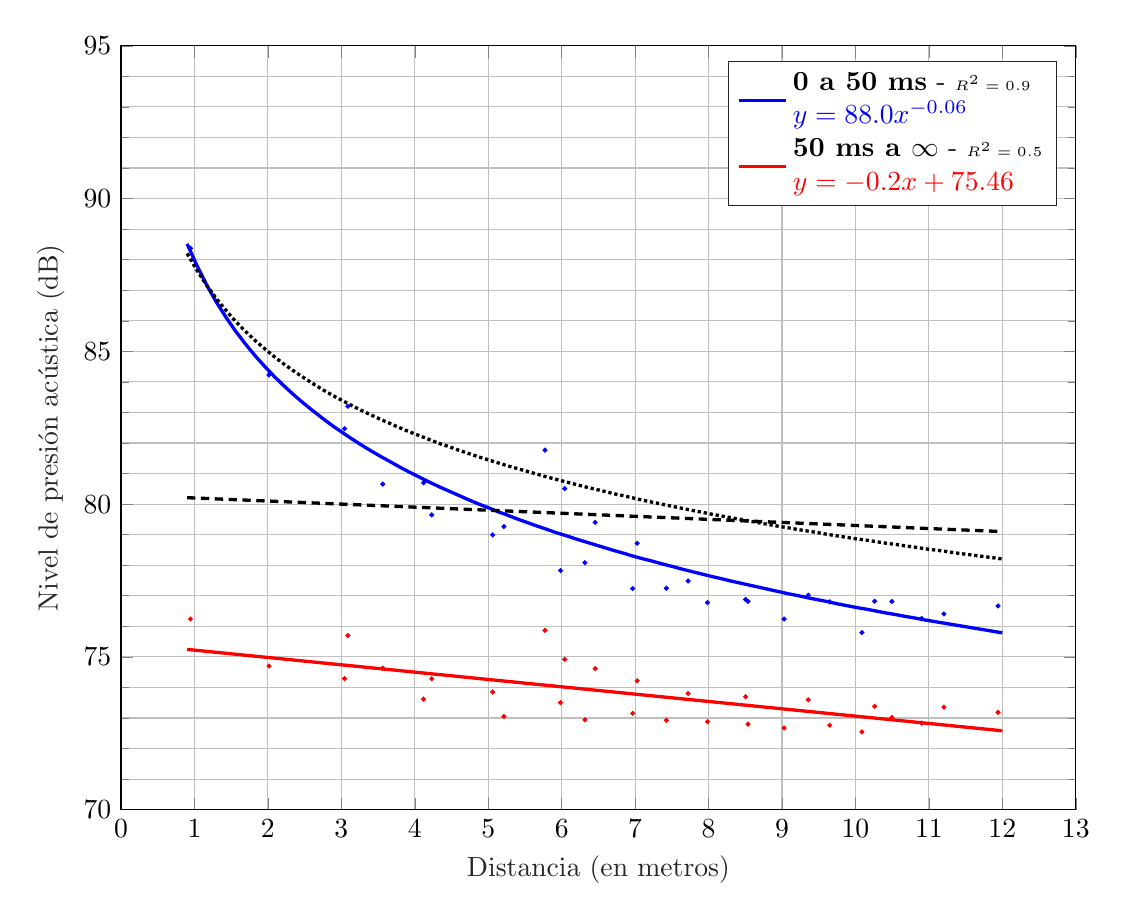
\begin{tikzpicture}

\begin{axis}[%
width=\textwidth,
height=0.8\textwidth,
at={(0\textwidth,0\textwidth)},
scale only axis,
xmin=0,
xmax=13,
xlabel style={font=\color{white!15!black}},
xlabel={Distancia (en metros)},
ymin=70,
ymax=95,
ylabel style={font=\color{white!15!black}},
ylabel={Nivel de presión acústica (dB)},
axis background/.style={fill=white},
xmajorgrids,
xminorgrids,
ymajorgrids,
yminorgrids,
minor y tick num= 4,
legend style={legend cell align=left, align=left, draw=white!15!black}
]
% Curvas EASE
\addplot[color=blue,domain=0.9:12, samples=85,line width=1.2]{87.96*x^(-0.06)};
\addlegendentry{\textbf{0 a 50 ms} - \tiny{$R^2 = 0.9$}\\$\color{blue}y = 88.0·x^{-0.06}$}

\addplot[color=red,domain=0.9:12, samples=85,line width=1.2]{-0.24*x+75.46};
\addlegendentry{\textbf{50 ms a $\infty$} - \tiny{$R^2 = 0.5$}\\$\color{red}y = -0.2·x+75.46$}

% Curvas insitu
\addplot[color=black,densely dotted,line width=1.2pt,domain=0.9:12, samples=85]{81.97*x^(-0.05)+5.8};
\addplot[color=black,densely dashed,line width=1.2pt,domain=0.9:12, samples=85]{-0.1*x+74.5+5.8};

% Puntos
\addplot [color=blue, only marks,mark size=0.7pt]
  table[row sep=crcr]{%
0.945832966226067	88.3682361772189\\
2.01558924386890	84.2291706003832\\
3.04292622322658	82.4668549521070\\
3.08781476128346	83.2029970283003\\
3.56407070636933	80.6540733671014\\
4.11885906532379	80.6973572178475\\
4.23076825174814	79.6488729752191\\
5.06013833802990	78.9922829780122\\
5.21338661524349	79.2638568751166\\
5.77252977471749	81.7679073934008\\
5.98493107729738	77.8231571292173\\
6.04070360140274	80.5059625653217\\
6.31685048105462	78.0808143861506\\
6.45653932071973	79.3980859974177\\
6.96725196903342	77.2361311923270\\
7.02797979507625	78.7160630706607\\
7.42526767194288	77.2475666290034\\
7.72055049850721	77.4826461787419\\
7.98590007450632	76.7744119941775\\
8.50471045950419	76.8788490298862\\
8.53670896774630	76.8177175788655\\
9.02858792946051	76.2392456191651\\
9.35746226281464	77.0170446009200\\
9.65012953280939	76.7992546854551\\
10.0878639959111	75.7945503823589\\
10.2617201287114	76.8209111400215\\
10.4960706933595	76.8124711264967\\
10.8998853204976	76.2550733066322\\
11.2050211958746	76.4040325602856\\
11.9413148354777	76.6665578031064\\
};

\addplot [color=red, only marks,mark size=0.7pt]
  table[row sep=crcr]{%
0.945832966226067	76.2396363848670\\
2.01558924386890	74.6998074599683\\
3.04292622322658	74.2884368741902\\
3.08781476128346	75.6997458549146\\
3.56407070636933	74.6323479110658\\
4.11885906532379	73.6161328802466\\
4.23076825174814	74.2832904572305\\
5.06013833802990	73.8482743054767\\
5.21338661524349	73.0472847246087\\
5.77252977471749	75.8649938279239\\
5.98493107729738	73.5022852375788\\
6.04070360140274	74.9174519410973\\
6.31685048105462	72.9392193708742\\
6.45653932071973	74.6166522206872\\
6.96725196903342	73.1530983399761\\
7.02797979507625	74.2157331821576\\
7.42526767194288	72.9261505004440\\
7.72055049850721	73.7999541831440\\
7.98590007450632	72.8778276092374\\
8.50471045950419	73.6940274223339\\
8.53670896774630	72.7973708807318\\
9.02858792946051	72.6717170303752\\
9.35746226281464	73.5949579057793\\
9.65012953280939	72.7609779382917\\
10.0878639959111	72.5430723749307\\
10.2617201287114	73.3813504626970\\
10.4960706933595	73.0180229693039\\
10.8998853204976	72.8316501605893\\
11.2050211958746	73.3517691608670\\
11.9413148354777	73.1824678093616\\
  };
\end{axis}
\end{tikzpicture}%%
    }
    \caption{Fuente en la esquina}%
    \end{subfigure}%
    \hspace{1.9cm}%
    \begin{subfigure}[b]{0.4\textwidth}%
    	\centering%
        {\scalefont{0.8}%
    %%%%%%%%%%%%%%%%%%%%%%%%%%%%%%%%%%%%%%%%%%%%%%%%%%%%%%%%%%%%%%%%%%%%%%%%
% Escuela Politécnica Superior de la Universidad de Alicante
% Realizado por: Jose Manuel Requena Plens
% Contacto: info@jmrplens.com / Telegram:@jmrplens
%%%%%%%%%%%%%%%%%%%%%%%%%%%%%%%%%%%%%%%%%%%%%%%%%%%%%%%%%%%%%%%%%%%%%%%%

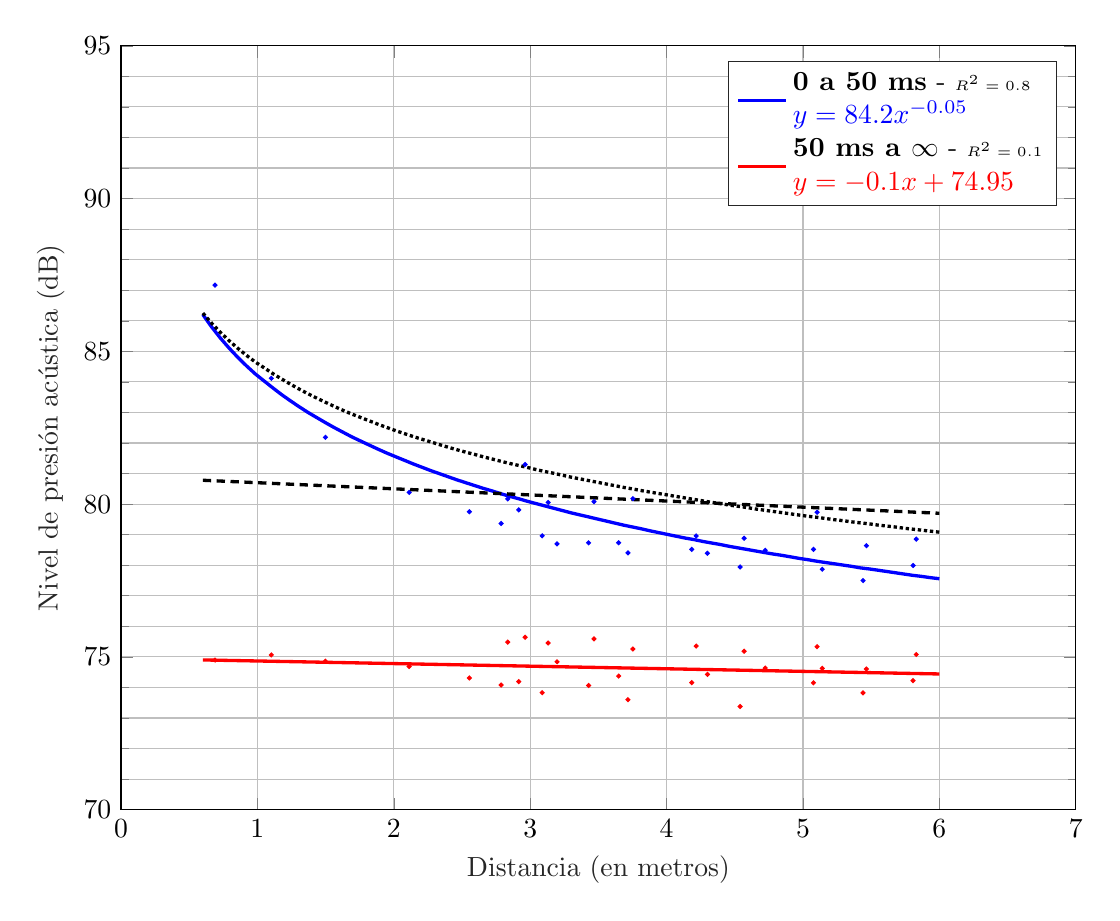
\begin{tikzpicture}

\begin{axis}[%
width=\textwidth,
height=0.8\textwidth,
at={(0\textwidth,0\textwidth)},
scale only axis,
xmin=0,
xmax=7,
xlabel style={font=\color{white!15!black}},
xlabel={Distancia (en metros)},
ymin=70,
ymax=95,
ylabel style={font=\color{white!15!black}},
ylabel={Nivel de presión acústica (dB)},
axis background/.style={fill=white},
xmajorgrids,
xminorgrids,
ymajorgrids,
yminorgrids,
minor y tick num= 4,
legend style={legend cell align=left, align=left, draw=white!15!black}
]
% Curvas EASE
\addplot[color=blue,domain=0.6:6, samples=85,line width=1.2]{84.20*x^(-0.046)};
\addlegendentry{\textbf{0 a 50 ms} - \tiny{$R^2 = 0.8$}\\$\color{blue}y = 84.2·x^{-0.05}$}

\addplot[color=red,domain=0.6:6, samples=85,line width=1.2]{-0.085*x+74.95};
\addlegendentry{\textbf{50 ms a $\infty$} - \tiny{$R^2 = 0.1$}\\$\color{red}y = -0.1·x+74.95$}

% Curvas in situ
\addplot[color=black,densely dotted,line width=1.2pt,domain=0.6:6, samples=85]{80*x^(-0.04)+4.6};
\addplot[color=black,densely dashed,line width=1.2pt,domain=0.6:6, samples=85]{-0.2*x+76.3+4.6};

% Puntos
\addplot [color=blue, only marks,mark size=0.7pt]
  table[row sep=crcr]{%
0.689492567037528	87.1678881319192\\
1.10208892563168	84.1165563459516\\
1.49833240637717	82.1847846378159\\
2.11248668634858	80.3825860852206\\
2.55409475157051	79.7499124974280\\
2.78664673039121	79.3667594554426\\
2.83511904511962	80.1691036472047\\
2.91626473421053	79.8107789453695\\
2.96261708629381	81.2962706330534\\
3.08787953132890	78.9610504227305\\
3.13169283295792	80.0551789689806\\
3.19677962956473	78.6994459080520\\
3.42820652820101	78.7315251657904\\
3.46772259559498	80.0817675993113\\
3.64836949883095	78.7344352012910\\
3.71663826596025	78.4026434296394\\
3.75311870315875	80.1768717051253\\
4.18442349673166	78.5159183345488\\
4.21685902064558	78.9590967022620\\
4.29941856534113	78.3913859061579\\
4.53878838458019	77.9424192579992\\
4.56870878914382	78.8813591154629\\
4.72298634340605	78.4870819475297\\
5.07690850813760	78.5190868467895\\
5.10367514640186	79.7316236495648\\
5.14125471067132	77.8666846191468\\
5.44027572830643	77.4974042519682\\
5.46526303118157	78.6384552124610\\
5.80710771382794	77.9892449321896\\
5.83052313261855	78.8526133593289\\
  };
  
  \addplot [color=red, only marks,mark size=0.7pt]
  table[row sep=crcr]{%
0.689492567037528	74.8956050162762\\
1.10208892563168	75.0627995710503\\
1.49833240637717	74.8603183887478\\
2.11248668634858	74.6845194840402\\
2.55409475157051	74.3092374727581\\
2.78664673039121	74.0778295615781\\
2.83511904511962	75.4835224537465\\
2.91626473421053	74.1891089179431\\
2.96261708629381	75.6398059531280\\
3.08787953132890	73.8278791984142\\
3.13169283295792	75.4544460624605\\
3.19677962956473	74.8392327702789\\
3.42820652820101	74.0635554547840\\
3.46772259559498	75.5893035097754\\
3.64836949883095	74.3702747477762\\
3.71663826596025	73.5979257690534\\
3.75311870315875	75.2568692949836\\
4.18442349673166	74.1545231838629\\
4.21685902064558	75.3525822366600\\
4.29941856534113	74.4268175950121\\
4.53878838458019	73.3756171633836\\
4.56870878914382	75.1849676241943\\
4.72298634340605	74.6336274218104\\
5.07690850813760	74.1514417003351\\
5.10367514640186	75.3339594086641\\
5.14125471067132	74.6232480840075\\
5.44027572830643	73.8223032378054\\
5.46526303118157	74.6028437546984\\
5.80710771382794	74.2216309739673\\
5.83052313261855	75.0766435298864\\
  };
\end{axis}
\end{tikzpicture}%%
    }
    \caption{Fuente en el centro}%
    \end{subfigure}
    \caption{Campos acústicos en el aula EP/0-26M con mobiliario simulado en EASE. Se muestran las curvas in situ (negro) con el nivel global modificado para poder comparar.}
    \label{graf:easeepsmob}%
\end{figure}
\FloatBarrier 

\begin{figure}[ht]
    \begin{subfigure}[b]{0.4\textwidth}
    	\centering%
         {\scalefont{0.8}%
    %%%%%%%%%%%%%%%%%%%%%%%%%%%%%%%%%%%%%%%%%%%%%%%%%%%%%%%%%%%%%%%%%%%%%%%%
% Escuela Politécnica Superior de la Universidad de Alicante
% Realizado por: Jose Manuel Requena Plens
% Contacto: info@jmrplens.com / Telegram:@jmrplens
%%%%%%%%%%%%%%%%%%%%%%%%%%%%%%%%%%%%%%%%%%%%%%%%%%%%%%%%%%%%%%%%%%%%%%%%

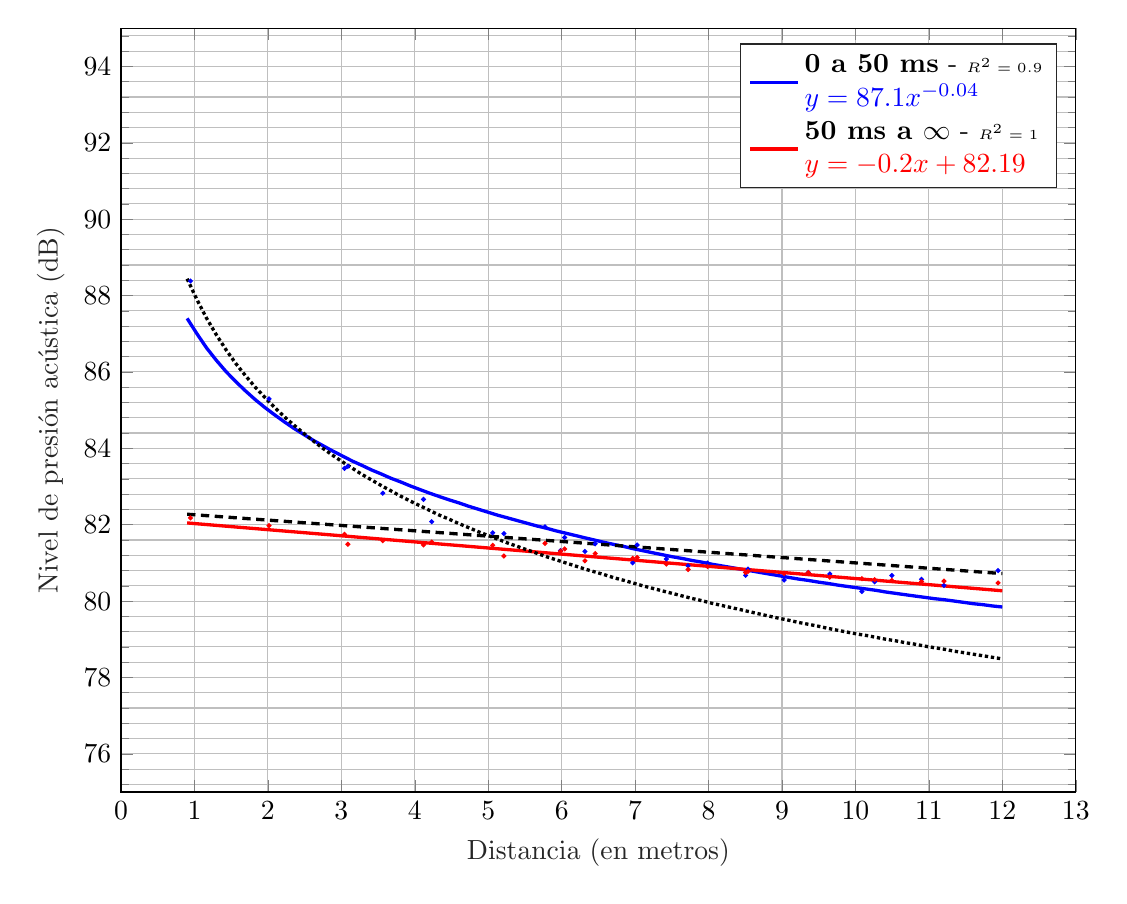
\begin{tikzpicture}

\begin{axis}[%
width=\textwidth,
height=0.8\textwidth,
at={(0\textwidth,0\textwidth)},
scale only axis,
xmin=0,
xmax=13,
xlabel style={font=\color{white!15!black}},
xlabel={Distancia (en metros)},
ymin=75,
ymax=95,
ylabel style={font=\color{white!15!black}},
ylabel={Nivel de presión acústica (dB)},
axis background/.style={fill=white},
xmajorgrids,
xminorgrids,
ymajorgrids,
yminorgrids,
minor y tick num= 4,
legend style={legend cell align=left, align=left, draw=white!15!black}
]
% Curvas EASE
\addplot[color=blue,domain=0.9:12, samples=85,line width=1.2]{87.08*x^(-0.035)};
\addlegendentry{\textbf{0 a 50 ms} - \tiny{$R^2 = 0.9$}\\$\color{blue}y = 87.1·x^{-0.04}$}

\addplot[color=red,domain=0.9:12, samples=85,line width=1.2]{-0.16*x+82.19};
\addlegendentry{\textbf{50 ms a $\infty$} - \tiny{$R^2 = 1$}\\$\color{red}y = -0.2·x+82.19$}

% Curvas insitu
\addplot[color=black,densely dotted,line width=1.2pt,domain=0.9:12, samples=85]{81.61*x^(-0.05)+6.4};
\addplot[color=black,densely dashed,line width=1.2pt,domain=0.9:12, samples=85]{-0.14*x+76+6.4};

% Puntos
\addplot [color=blue, only marks,mark size=0.7pt]
  table[row sep=crcr]{%
0.945832966226067	88.3808391236599\\
2.01558924386890	85.2936795349521\\
3.04292622322658	83.4748783371691\\
3.08781476128346	83.5272045055965\\
3.56407070636933	82.8240090793044\\
4.11885906532379	82.6625494089014\\
4.23076825174814	82.0778955814787\\
5.06013833802990	81.7870262070404\\
5.21338661524349	81.7665926486219\\
5.77252977471749	81.9443544059675\\
5.98493107729738	81.3208054322234\\
6.04070360140274	81.6650826299988\\
6.31685048105462	81.2999367072749\\
6.45653932071973	81.4997990721067\\
6.96725196903342	81.0025149070337\\
7.02797979507625	81.4677403312375\\
7.42526767194288	81.1018723483650\\
7.72055049850721	80.9235270091036\\
7.98590007450632	80.9954788950488\\
8.50471045950419	80.6731668471498\\
8.53670896774630	80.8362954223367\\
9.02858792946051	80.5508547076089\\
9.35746226281464	80.7488175613742\\
9.65012953280939	80.7098929463617\\
10.0878639959111	80.2520438800622\\
10.2617201287114	80.5048862291226\\
10.4960706933595	80.6697126771525\\
10.8998853204976	80.5700129654216\\
11.2050211958746	80.4092875811931\\
11.9413148354777	80.7996545494746\\
};

\addplot [color=red, only marks,mark size=0.7pt]
  table[row sep=crcr]{%
0.945832966226067	82.1762817068517\\
2.01558924386890	81.9749784864042\\
3.04292622322658	81.7480751216254\\
3.08781476128346	81.4879654117737\\
3.56407070636933	81.5826814679269\\
4.11885906532379	81.4704552735545\\
4.23076825174814	81.5454353466553\\
5.06013833802990	81.4595895500597\\
5.21338661524349	81.1794515116566\\
5.77252977471749	81.5109656456417\\
5.98493107729738	81.3075137554158\\
6.04070360140274	81.3663646693337\\
6.31685048105462	81.0543473658963\\
6.45653932071973	81.2451624624217\\
6.96725196903342	81.1187342986678\\
7.02797979507625	81.1404282911666\\
7.42526767194288	80.9681387400627\\
7.72055049850721	80.8269321373207\\
7.98590007450632	80.9042299768582\\
8.50471045950419	80.7491795550527\\
8.53670896774630	80.7793706338611\\
9.02858792946051	80.7196944369790\\
9.35746226281464	80.7432806230875\\
9.65012953280939	80.6287695808118\\
10.0878639959111	80.5865014414949\\
10.2617201287114	80.5608617896108\\
10.4960706933595	80.5417583543006\\
10.8998853204976	80.5121065468405\\
11.2050211958746	80.5229843812398\\
11.9413148354777	80.4741526201567\\
  };
\end{axis}
\end{tikzpicture}%%
    }
    \caption{Fuente en la esquina}%
    \end{subfigure}%
    \hspace{1.9cm}%
    \begin{subfigure}[b]{0.4\textwidth}%
    	\centering%
        {\scalefont{0.8}%
    %%%%%%%%%%%%%%%%%%%%%%%%%%%%%%%%%%%%%%%%%%%%%%%%%%%%%%%%%%%%%%%%%%%%%%%%
% Escuela Politécnica Superior de la Universidad de Alicante
% Realizado por: Jose Manuel Requena Plens
% Contacto: info@jmrplens.com / Telegram:@jmrplens
%%%%%%%%%%%%%%%%%%%%%%%%%%%%%%%%%%%%%%%%%%%%%%%%%%%%%%%%%%%%%%%%%%%%%%%%

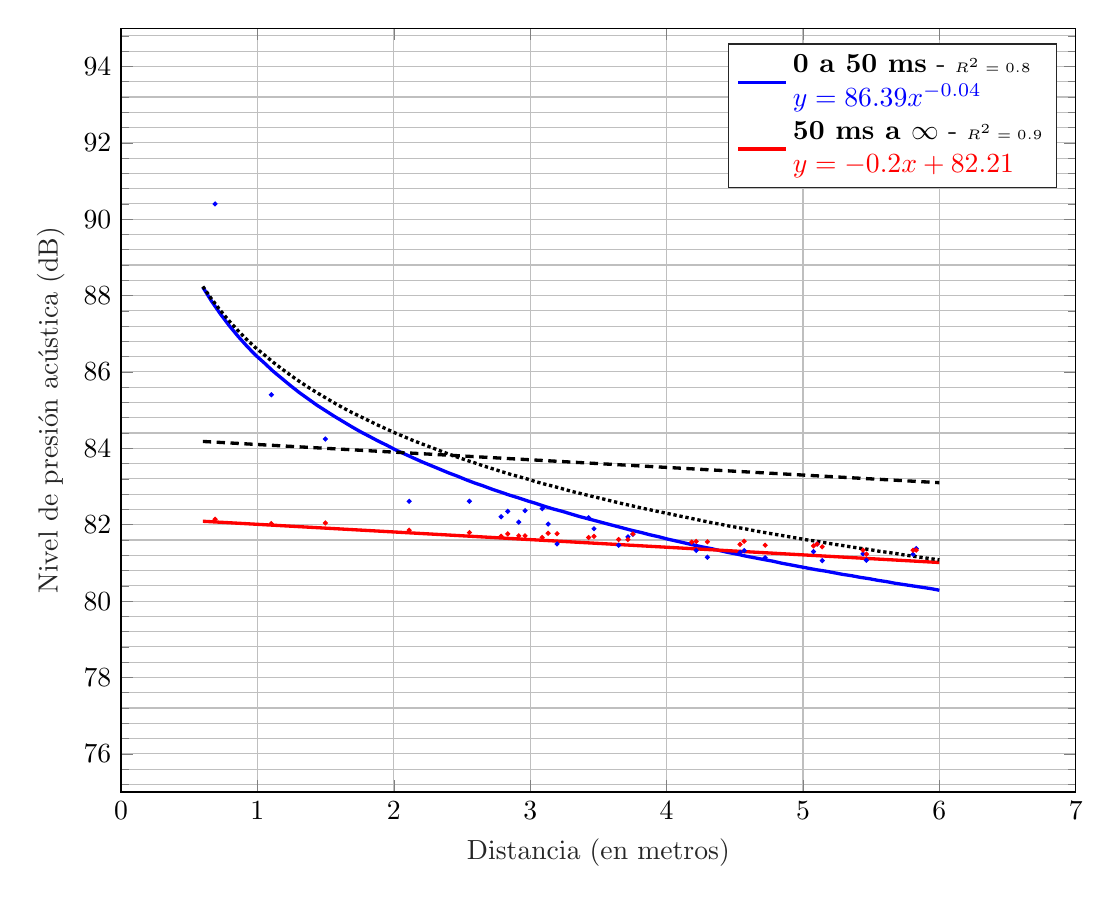
\begin{tikzpicture}

\begin{axis}[%
width=\textwidth,
height=0.8\textwidth,
at={(0\textwidth,0\textwidth)},
scale only axis,
xmin=0,
xmax=7,
xlabel style={font=\color{white!15!black}},
xlabel={Distancia (en metros)},
ymin=75,
ymax=95,
ylabel style={font=\color{white!15!black}},
ylabel={Nivel de presión acústica (dB)},
axis background/.style={fill=white},
xmajorgrids,
xminorgrids,
ymajorgrids,
yminorgrids,
minor y tick num= 4,
legend style={legend cell align=left, align=left, draw=white!15!black}
]
% Curvas EASE
\addplot[color=blue,domain=0.6:6, samples=85,line width=1.2]{86.39*x^(-0.041)};
\addlegendentry{\textbf{0 a 50 ms} - \tiny{$R^2 = 0.8$}\\$\color{blue}y = 86.39·x^{-0.04}$}

\addplot[color=red,domain=0.6:6, samples=85,line width=1.2]{-0.2*x+82.21};
\addlegendentry{\textbf{50 ms a $\infty$} - \tiny{$R^2 = 0.9$}\\$\color{red}y = -0.2·x+82.21$}

% Curvas in situ
\addplot[color=black,densely dotted,line width=1.2pt,domain=0.6:6, samples=85]{79.89*x^(-0.04)+6.7};
\addplot[color=black,densely dashed,line width=1.2pt,domain=0.6:6, samples=85]{-0.2*x+77.6+6.7};

% Puntos
\addplot [color=blue, only marks,mark size=0.7pt]
  table[row sep=crcr]{%
0.689492567037528	90.3982646553281\\
1.10208892563168	85.4021853316195\\
1.49833240637717	84.2425825118207\\
2.11248668634858	82.6116352718178\\
2.55409475157051	82.6135122913565\\
2.78664673039121	82.2069902990955\\
2.83511904511962	82.3492400917929\\
2.91626473421053	82.0680524605599\\
2.96261708629381	82.3683576537562\\
3.08787953132890	82.4214071828821\\
3.13169283295792	82.0154843359460\\
3.19677962956473	81.4951924998070\\
3.42820652820101	82.1830625473700\\
3.46772259559498	81.8939660289482\\
3.64836949883095	81.4634891242453\\
3.71663826596025	81.6830817762083\\
3.75311870315875	81.7509835368211\\
4.18442349673166	81.5268252555827\\
4.21685902064558	81.3263223641795\\
4.29941856534113	81.1487112320415\\
4.53878838458019	81.2735704456450\\
4.56870878914382	81.3211075371412\\
4.72298634340605	81.1341656558285\\
5.07690850813760	81.2952042735866\\
5.10367514640186	81.4959826351208\\
5.14125471067132	81.0587718340490\\
5.44027572830643	81.2363689965190\\
5.46526303118157	81.0686463752940\\
5.80710771382794	81.2251663600713\\
5.83052313261855	81.3736867303669\\
  };
  
  \addplot [color=red, only marks,mark size=0.7pt]
  table[row sep=crcr]{%
0.689492567037528	82.1423350384191\\
1.10208892563168	82.0297157546384\\
1.49833240637717	82.0460870818860\\
2.11248668634858	81.8568097062743\\
2.55409475157051	81.7931265121477\\
2.78664673039121	81.6981070013399\\
2.83511904511962	81.7594343944194\\
2.91626473421053	81.7100391109355\\
2.96261708629381	81.7082789264959\\
3.08787953132890	81.6659553549367\\
3.13169283295792	81.7766272909335\\
3.19677962956473	81.7637826320174\\
3.42820652820101	81.6632557687887\\
3.46772259559498	81.6945279991275\\
3.64836949883095	81.6121855876210\\
3.71663826596025	81.6110145624761\\
3.75311870315875	81.7582478723122\\
4.18442349673166	81.5449185456124\\
4.21685902064558	81.5624088971591\\
4.29941856534113	81.5514551505769\\
4.53878838458019	81.4852204366460\\
4.56870878914382	81.5662619687015\\
4.72298634340605	81.4625715488726\\
5.07690850813760	81.4456890191893\\
5.10367514640186	81.4933895955345\\
5.14125471067132	81.4217817790589\\
5.44027572830643	81.3309756894275\\
5.46526303118157	81.2287297336981\\
5.80710771382794	81.3305296547238\\
5.83052313261855	81.3336582166581\\
  };
\end{axis}
\end{tikzpicture}%%
    }
    \caption{Fuente en el centro}%
    \end{subfigure}
    \caption{Campos acústicos en el aula EP/0-26M sin mobiliario simulado en EASE. Se muestran las curvas in situ (negro) con el nivel global modificado para poder comparar.}
    \label{graf:easeepsnomob}%
\end{figure}
\FloatBarrier 

Como en todos los modelos, cuando se incluye el mobiliario el campo perjudicial queda muy por debajo de lo obtenido en las medidas in situ. En cambio, en los cálculos sin mobiliario con la fuente en la esquina son muy similares a las medidas in situ, con la fuente en el centro el campo directo es similar a las medidas in situ pero el perjudicial queda ligeramente por debajo.

\section{Selección de modelos}
\label{modelosvalidados}
En el apartado anterior se han visualizado los resultados de cada uno de los modelos, pudiendo eliminar las opciones que distan mucho de las medidas in situ.
En primer lugar se ha observado que, a simple vista, CATT-Acoustic no se ajusta a los resultados buscados, por lo que ningún modelo realizado con CATT-Acoustic se utilizará en este trabajo.

En las simulaciones con EASE se han obtenido resultados correctos en los casos sin mobiliario, para confirmar la validez de estos modelos a continuación se muestran de nuevo las curvas anteriores añadiendo la información de errores producidos en la regresión de las curvas de los modelos. Las figuras \ref{graf:easeopnomobesquina-errores} y \ref{graf:easeopnomobcentro-errores} muestran los detalles de los campos acústicos del aula OP/S003, y las figuras \ref{graf:easeepsnomobesquina-errores} y \ref{graf:easeepsnomobcentro-errores} muestran los detalles de los campos acústicos del aula EP/0-26M.


La primera condición para que las curvas obtenidas mediante simulación sean consideradas iguales a las curvas de las medidas in situ es que, dentro del margen de error de las curvas simuladas se encuentren las curvas de las medidas in situ o, en su defecto, que dentro de ese margen se encuentren los márgenes de error de las curvas in situ. La segunda condición, cuando la primera no se cumple, es que la diferencia máxima entre curvas no supere el 5\% del valor de alguna de ellas, es decir, un nivel de confianza del 95\%.
\begin{figure}[ht]
	\centering%
     {\scalefont{0.8}%
    %%%%%%%%%%%%%%%%%%%%%%%%%%%%%%%%%%%%%%%%%%%%%%%%%%%%%%%%%%%%%%%%%%%%%%%%
% Escuela Politécnica Superior de la Universidad de Alicante
% Realizado por: Jose Manuel Requena Plens
% Contacto: info@jmrplens.com / Telegram:@jmrplens
%%%%%%%%%%%%%%%%%%%%%%%%%%%%%%%%%%%%%%%%%%%%%%%%%%%%%%%%%%%%%%%%%%%%%%%%

\begin{tikzpicture}

\begin{axis}[%
width=0.8\textwidth,
height=0.35\textwidth,
at={(0\textwidth,0\textwidth)},
scale only axis,
xmin=0,
xmax=19,
xlabel style={font=\color{white!15!black}},
xlabel={Distancia (en metros)},
ymin=72,
ymax=90,
minor x tick num= 1,
minor y tick num= 4,
ylabel style={font=\color{white!15!black}},
ylabel={Nivel de presión acústica (dB)},
axis background/.style={fill=white},
%xmajorgrids,
%xminorgrids,
%ymajorgrids,
%yminorgrids,
grid=both,
legend style={legend cell align=left, align=left, draw=white!15!black}
]
% Curvas EASE
\addplot[color=blue,line width=1.2pt,domain=1:18.5, samples=85]{87.95*x^(-0.05187)};


\addplot[color=red,line width=1.2pt,domain=1:18.5, samples=85]{-0.1878*x+79.97};


% Curvas insitu
\addplot[color=black,densely dotted,line width=1.2pt,domain=1:18.5, samples=85]{82.41*x^(-0.04889)+5.5};

\addplot[color=black, dashed,line width=1.2pt,domain=1:18.5, samples=85]{-0.1372*x+75.63+5.5};

\addlegendentry{\scriptsize{\textbf{0 a 50 ms}} - EASE}
\addlegendentry{\scriptsize{\textbf{50 ms a $\infty$}} - EASE}
\addlegendentry{\scriptsize{\textbf{0 a 50 ms}} - In situ}
\addlegendentry{\scriptsize{\textbf{50 ms a $\infty$}} - In situ}
% Errores
\addplot[color=blue, only marks,,mark size=1.8pt,mark=x,error bars/.cd,y dir=both, y explicit,error bar style={line width=1pt}] 
		table [x=x,y=y, y error plus=ymas, y error minus=ymenos]
			{archivos/graficastikz/OpvaciaEsquinaUtilErrores.dat};
			
\addplot[color=red, only marks,mark size=1.8pt,mark=x,error bars/.cd,y dir=both, y explicit,error bar style={line width=1pt}] 
		table [x=x,y=y, y error plus=ymas, y error minus=ymenos]
			{archivos/graficastikz/OpvaciaEsquinaPerjudicialErrores.dat};

\addplot[color=black, only marks,mark size=1.8pt,mark=x,error bars/.cd,y dir=both, y explicit,error mark=triangle,error bar style={densely dotted,line width=1pt}] 
		table [x=x,y=y, y error plus=ymas, y error minus=ymenos]
			{archivos/graficastikz/OpllenaCentroUtilErroresinsitu.dat};
			
\addplot[color=black, only marks,mark size=1.8pt,mark=x,error bars/.cd,y dir=both, y explicit,error mark=diamond,error bar style={ dashed,line width=1pt}] 
		table [x=x,y=y, y error plus=ymas, y error minus=ymenos]
			{archivos/graficastikz/OpllenaCentroPerjudicialErroresinsitu.dat};




%% Puntos
%\addplot [color=blue, only marks,mark size=0.7pt]
%  table[row sep=crcr]{%
%1.17046999107196	87.1277550611968\\
%2.78747197295327	83.4623086675921\\
%4.04598566482878	82.2179401358662\\
%4.77179211617606	81.5257517559293\\
%5.44357419348722	80.4045039689526\\
%6.68075594525051	79.6754872626557\\
%7.02637886823647	80.2469029713596\\
%7.46793144049944	79.7283523968088\\
%7.66615940350838	78.6559229050811\\
%8.58894638474359	78.3326673816969\\
%8.81093071133805	78.7617201801592\\
%10.1498768465435	77.1663192028700\\
%10.3329569823938	76.8891694043067\\
%10.8637010268140	76.8468643393087\\
%12.2890194889584	77.9181962233661\\
%12.6400158227749	76.1735762643118\\
%13.2200605142337	76.8612684404271\\
%14.4142290810157	76.9428881306448\\
%15.1334067545943	76.3340029077443\\
%15.6211395230950	76.4290703842402\\
%16.6439178080162	75.5728813031650\\
%17.1295067062657	76.4126252632454\\
%17.5618905588208	75.9345334655598\\
%18.4775539506722	76.6630383745993\\
%};
%
%\addplot [color=red, only marks,mark size=0.7pt]
%  table[row sep=crcr]{%
%1.17046999107196	80.3231940709341\\
%2.78747197295327	79.5902397011391\\
%4.04598566482878	79.0120257322755\\
%4.77179211617606	79.0732056591827\\
%5.44357419348722	78.5794103477747\\
%6.68075594525051	78.7408951295518\\
%7.02637886823647	78.4806520089487\\
%7.46793144049944	78.6186486954362\\
%7.66615940350838	78.2622920553155\\
%8.58894638474359	78.1230323668705\\
%8.81093071133805	78.6111774265353\\
%10.1498768465435	77.8093052083963\\
%10.3329569823938	77.9430570409649\\
%10.8637010268140	77.8977458350415\\
%12.2890194889584	77.9283000590244\\
%12.6400158227749	77.4366536941934\\
%13.2200605142337	77.5555167518319\\
%14.4142290810157	77.5382759101964\\
%15.1334067545943	76.9569768837744\\
%15.6211395230950	77.1695938485288\\
%16.6439178080162	76.8237758577911\\
%17.1295067062657	76.5974351112101\\
%17.5618905588208	76.8959648117646\\
%18.4775539506722	76.5579088024192\\
%  };
\end{axis}
\end{tikzpicture}%%
    }
    \caption{Verificación del campo acústico en el aula OP/S003 con fuente en la esquina y sin mobiliario simulado en EASE.}%
     \label{graf:easeopnomobesquina-errores}%
\end{figure}

En el aula OP/S003 sin mobiliario y fuente en la esquina (figura \ref{graf:easeopnomobesquina-errores}), la curva del campo útil simulado se encuentra dentro del margen de error de la curva simulada, por el contrario, la curva del campo perjudicial no se encuentra dentro del margen de error ni de la suma de los márgenes de simulación e in situ, hay una diferencia aproximada menor a 1 dB ($<$5\%) entre ambas curvas. En conclusión, aún teniendo la diferencia aproximada de 1 dB en el campo perjudicial, estas curvas se pueden considerar iguales.

\begin{figure}[ht]
    \centering%
    {\scalefont{0.8}%
    %%%%%%%%%%%%%%%%%%%%%%%%%%%%%%%%%%%%%%%%%%%%%%%%%%%%%%%%%%%%%%%%%%%%%%%%
% Escuela Politécnica Superior de la Universidad de Alicante
% Realizado por: Jose Manuel Requena Plens
% Contacto: info@jmrplens.com / Telegram:@jmrplens
%%%%%%%%%%%%%%%%%%%%%%%%%%%%%%%%%%%%%%%%%%%%%%%%%%%%%%%%%%%%%%%%%%%%%%%%

\begin{tikzpicture}

\begin{axis}[%
width=0.8\textwidth,
height=0.35\textwidth,
at={(0\textwidth,0\textwidth)},
scale only axis,
xmin=0,
xmax=10,
xlabel style={font=\color{white!15!black}},
xlabel={Distancia (en metros)},
minor x tick num= 1,
minor y tick num= 1,
ymin=75,
ymax=88,
ylabel style={font=\color{white!15!black}},
ylabel={Nivel de presión acústica (dB)},
axis background/.style={fill=white},
grid=both,
%xmajorgrids,
%xminorgrids,
%ymajorgrids,
%yminorgrids,
legend style={legend cell align=left, align=left, draw=white!15!black}
]
% Curvas EASE
\addplot[color=blue,line width=1.2pt,domain=0.7:9.2, samples=85]{85.18*x^(-0.047)};


\addplot[color=red,line width=1.2pt,domain=0.7:9.2, samples=85]{-0.18*x+79.77};


% Curvas in situ
\addplot[color=black,densely dotted,line width=1.2pt,domain=0.7:9.2, samples=85]{77.23*x^(-0.03336)+8.4};
\addplot[color=black, dashed,line width=1.2pt,domain=0.7:9.2, samples=85]{-0.199*x+75.06+8.4};

\addlegendentry{\scriptsize{\textbf{0 a 50 ms}} - EASE}
\addlegendentry{\scriptsize{\textbf{50 ms a $\infty$}} - EASE}
\addlegendentry{\scriptsize{\textbf{0 a 50 ms}} - In situ}
\addlegendentry{\scriptsize{\textbf{50 ms a $\infty$}} - In situ}

% Errores
\addplot[color=blue, only marks,,mark size=1.8pt,mark=x,error bars/.cd,y dir=both, y explicit,error bar style={line width=1pt}] 
		table [x=x,y=y, y error plus=ymas, y error minus=ymenos]
			{archivos/graficastikz/OpvaciaCentroUtilErrores.dat};
			
\addplot[color=red, only marks,mark size=1.8pt,mark=x,error bars/.cd,y dir=both, y explicit,error bar style={line width=1pt}] 
		table [x=x,y=y, y error plus=ymas, y error minus=ymenos]
			{archivos/graficastikz/OpvaciaCentroPerjudicialErrores.dat};
			
\addplot[color=black, only marks,mark size=1.8pt,mark=x,error bars/.cd,y dir=both, y explicit,error mark=triangle,error bar style={densely dotted,line width=1pt}] 
		table [x=x,y=y, y error plus=ymas, y error minus=ymenos]
			{archivos/graficastikz/OpvaciaCentroUtilErroresinsitu.dat};
			
\addplot[color=black, only marks,mark size=1.8pt,mark=x,error bars/.cd,y dir=both, y explicit,error mark=diamond,error bar style={ dashed,line width=1pt}] 
		table [x=x,y=y, y error plus=ymas, y error minus=ymenos]
			{archivos/graficastikz/OpvaciaCentroPerjudicialErroresinsitu.dat};
			

% Puntos
%\addplot [color=blue, only marks,mark size=0.7pt]
%  table[row sep=crcr]{%
% 0.911043357914430	86.2772796781886\\
%1.60623784042090	84.1056446478500\\
%3.03809150619266	80.7162943773909\\
%3.22955105239103	79.9791235432895\\
%3.31360830515618	80.1257164588809\\
%3.40293990543471	80.1549543981309\\
%3.48998567332303	80.3976116923752\\
%3.85259652701915	79.0293836816767\\
%4.46989932772540	78.8058727354038\\
%4.60217339960154	78.8512802176443\\
%4.82104760399646	78.8496625245368\\
%4.94393567919325	78.6032259795649\\
%5.90169467187180	77.9558802268358\\
%6.57495247131110	77.8065806803430\\
%6.60151497763960	77.5670065559296\\
%6.66558324529819	77.9950758659912\\
%7.20971566707037	77.6179645821617\\
%7.29246186140181	77.2229572843838\\
%7.90126572138920	77.4832543472834\\
%8.41605608346332	77.6356061014582\\
%8.48704895708750	77.5171417313596\\
%8.60116271209887	77.3035533865362\\
%9.07634287585038	77.4993226551940\\
%9.14220979851152	77.3278313594281\\
%  };
%  
%  \addplot [color=red, only marks,mark size=0.7pt]
%  table[row sep=crcr]{%
%0.911043357914430	79.8951008237853\\
%1.60623784042090	79.6634802579777\\
%3.03809150619266	79.1311060267053\\
%3.22955105239103	79.0290689238144\\
%3.31360830515618	79.1915465704714\\
%3.40293990543471	78.9738863429516\\
%3.48998567332303	79.1574260253045\\
%3.85259652701915	78.9034083062506\\
%4.46989932772540	78.8673915409159\\
%4.60217339960154	78.9747462523916\\
%4.82104760399646	78.8249463712323\\
%4.94393567919325	78.8986754815038\\
%5.90169467187180	78.5761350266222\\
%6.57495247131110	78.4254000607376\\
%6.60151497763960	78.5015455533187\\
%6.66558324529819	78.7147432854439\\
%7.20971566707037	78.5621450983992\\
%7.29246186140181	78.6112877631831\\
%7.90126572138920	78.1512018038794\\
%8.41605608346332	78.2574617650506\\
%8.48704895708750	78.3698657405733\\
%8.60116271209887	78.1141880570530\\
%9.07634287585038	78.2003228792576\\
%9.14220979851152	78.2818430326449\\
%  };
\end{axis}
\end{tikzpicture}%%
    }
    \caption{Verificación del campo acústico en el aula OP/S003 con fuente en el centro y sin mobiliario simulado en EASE.}%
    \label{graf:easeopnomobcentro-errores}%
\end{figure}

Siguiendo en el caso del aula OP/S003 sin mobiliario pero ahora con fuente en el centro (figura \ref{graf:easeopnomobcentro-errores}), la curva del campo útil en general se encuentra dentro de la suma de los márgenes de error de simulación e in situ. El campo perjudicial queda aproximadamente 2 dB por debajo de lo esperado sin superar el margen del 5\%, por lo que las curvas se consideran iguales.

\begin{figure}[ht]
	\centering%
     {\scalefont{0.8}%
    %%%%%%%%%%%%%%%%%%%%%%%%%%%%%%%%%%%%%%%%%%%%%%%%%%%%%%%%%%%%%%%%%%%%%%%%
% Escuela Politécnica Superior de la Universidad de Alicante
% Realizado por: Jose Manuel Requena Plens
% Contacto: info@jmrplens.com / Telegram:@jmrplens
%%%%%%%%%%%%%%%%%%%%%%%%%%%%%%%%%%%%%%%%%%%%%%%%%%%%%%%%%%%%%%%%%%%%%%%%

\begin{tikzpicture}

\begin{axis}[%
width=0.8\textwidth,
height=0.35\textwidth,
at={(0\textwidth,0\textwidth)},
scale only axis,
xmin=0,
xmax=13,
xlabel style={font=\color{white!15!black}},
xlabel={Distancia (en metros)},
ymin=74,
ymax=90,
minor x tick num= 1,
minor y tick num= 4,
grid=both,
ylabel style={font=\color{white!15!black}},
ylabel={Nivel de presión acústica (dB)},
axis background/.style={fill=white},
%xmajorgrids,
%xminorgrids,
%ymajorgrids,
%yminorgrids,
legend style={legend cell align=left, align=left, draw=white!15!black}
]
% Curvas EASE
\addplot[color=blue,line width=1.2pt,domain=0.9:12, samples=85]{87.08*x^(-0.03497)};

\addplot[color=red,line width=1.2pt,domain=0.9:12, samples=85]{-0.1566*x+82.19};


% Curvas insitu
\addplot[color=black,densely dotted,line width=1.2pt,domain=0.9:12, samples=85]{81.61*x^(-0.04478)+5.4};
\addplot[color=black,dashed,line width=1.2pt,domain=0.9:12, samples=85]{-0.1274*x+76.03+5.4};

\addlegendentry{\scriptsize{\textbf{0 a 50 ms}} - EASE}
\addlegendentry{\scriptsize{\textbf{50 ms a $\infty$}} - EASE}
\addlegendentry{\scriptsize{\textbf{0 a 50 ms}} - In situ}
\addlegendentry{\scriptsize{\textbf{50 ms a $\infty$}} - In situ}

% Errores
\addplot[color=blue, only marks,,mark size=1.8pt,mark=x,error bars/.cd,y dir=both, y explicit,error bar style={line width=1pt}] 
		table [x=x,y=y, y error plus=ymas, y error minus=ymenos]
			{archivos/graficastikz/EpsvaciaEsquinaUtilErrores.dat};
			
\addplot[color=red, only marks,mark size=1.8pt,mark=x,error bars/.cd,y dir=both, y explicit,error bar style={line width=1pt}] 
		table [x=x,y=y, y error plus=ymas, y error minus=ymenos]
			{archivos/graficastikz/EpsvaciaEsquinaPerjudicialErrores.dat};
			
\addplot[color=black, only marks,mark size=1.8pt,mark=x,error bars/.cd,y dir=both, y explicit,error mark=triangle,error bar style={densely dotted,line width=1pt}] 
		table [x=x,y=y, y error plus=ymas, y error minus=ymenos]
			{archivos/graficastikz/EpsvaciaEsquinaUtilErroresinsitu.dat};
			
\addplot[color=black, only marks,mark size=1.8pt,mark=x,error bars/.cd,y dir=both, y explicit,error mark=diamond,error bar style={dashed,line width=1pt}] 
		table [x=x,y=y, y error plus=ymas, y error minus=ymenos]
			{archivos/graficastikz/EpsvaciaEsquinaPerjudicialErroresinsitu.dat};

% Puntos
%\addplot [color=blue, only marks,mark size=0.7pt]
%  table[row sep=crcr]{%
%0.945832966226067	88.3808391236599\\
%2.01558924386890	85.2936795349521\\
%3.04292622322658	83.4748783371691\\
%3.08781476128346	83.5272045055965\\
%3.56407070636933	82.8240090793044\\
%4.11885906532379	82.6625494089014\\
%4.23076825174814	82.0778955814787\\
%5.06013833802990	81.7870262070404\\
%5.21338661524349	81.7665926486219\\
%5.77252977471749	81.9443544059675\\
%5.98493107729738	81.3208054322234\\
%6.04070360140274	81.6650826299988\\
%6.31685048105462	81.2999367072749\\
%6.45653932071973	81.4997990721067\\
%6.96725196903342	81.0025149070337\\
%7.02797979507625	81.4677403312375\\
%7.42526767194288	81.1018723483650\\
%7.72055049850721	80.9235270091036\\
%7.98590007450632	80.9954788950488\\
%8.50471045950419	80.6731668471498\\
%8.53670896774630	80.8362954223367\\
%9.02858792946051	80.5508547076089\\
%9.35746226281464	80.7488175613742\\
%9.65012953280939	80.7098929463617\\
%10.0878639959111	80.2520438800622\\
%10.2617201287114	80.5048862291226\\
%10.4960706933595	80.6697126771525\\
%10.8998853204976	80.5700129654216\\
%11.2050211958746	80.4092875811931\\
%11.9413148354777	80.7996545494746\\
%};
%
%\addplot [color=red, only marks,mark size=0.7pt]
%  table[row sep=crcr]{%
%0.945832966226067	82.1762817068517\\
%2.01558924386890	81.9749784864042\\
%3.04292622322658	81.7480751216254\\
%3.08781476128346	81.4879654117737\\
%3.56407070636933	81.5826814679269\\
%4.11885906532379	81.4704552735545\\
%4.23076825174814	81.5454353466553\\
%5.06013833802990	81.4595895500597\\
%5.21338661524349	81.1794515116566\\
%5.77252977471749	81.5109656456417\\
%5.98493107729738	81.3075137554158\\
%6.04070360140274	81.3663646693337\\
%6.31685048105462	81.0543473658963\\
%6.45653932071973	81.2451624624217\\
%6.96725196903342	81.1187342986678\\
%7.02797979507625	81.1404282911666\\
%7.42526767194288	80.9681387400627\\
%7.72055049850721	80.8269321373207\\
%7.98590007450632	80.9042299768582\\
%8.50471045950419	80.7491795550527\\
%8.53670896774630	80.7793706338611\\
%9.02858792946051	80.7196944369790\\
%9.35746226281464	80.7432806230875\\
%9.65012953280939	80.6287695808118\\
%10.0878639959111	80.5865014414949\\
%10.2617201287114	80.5608617896108\\
%10.4960706933595	80.5417583543006\\
%10.8998853204976	80.5121065468405\\
%11.2050211958746	80.5229843812398\\
%11.9413148354777	80.4741526201567\\
%  };
\end{axis}
\end{tikzpicture}%%
    }
    \caption{Verificación del campo acústico en el aula EP/0-26M con fuente en la esquina y sin mobiliario simulado en EASE.}%
     \label{graf:easeepsnomobesquina-errores}%
\end{figure}
\FloatBarrier

En el aula EP/0-26M sin mobiliario y con fuente en la esquina (figura \ref{graf:easeepsnomobesquina-errores}) tanto la curva útil como la perjudicial se encuentran dentro de los márgenes de error, por lo que ambas curvas se consideran iguales.
\begin{figure}[ht]
    \centering%
    {\scalefont{0.8}%
    %%%%%%%%%%%%%%%%%%%%%%%%%%%%%%%%%%%%%%%%%%%%%%%%%%%%%%%%%%%%%%%%%%%%%%%%
% Escuela Politécnica Superior de la Universidad de Alicante
% Realizado por: Jose Manuel Requena Plens
% Contacto: info@jmrplens.com / Telegram:@jmrplens
%%%%%%%%%%%%%%%%%%%%%%%%%%%%%%%%%%%%%%%%%%%%%%%%%%%%%%%%%%%%%%%%%%%%%%%%

\begin{tikzpicture}

\begin{axis}[%
width=0.8\textwidth,
height=0.35\textwidth,
at={(0\textwidth,0\textwidth)},
scale only axis,
xmin=0,
xmax=6.5,
xlabel style={font=\color{white!15!black}},
xlabel={Distancia (en metros)},
ymin=78,
ymax=90,
minor x tick num= 1,
minor y tick num= 1,
grid=both,
ylabel style={font=\color{white!15!black}},
ylabel={Nivel de presión acústica (dB)},
axis background/.style={fill=white},
%xmajorgrids,
%xminorgrids,
%ymajorgrids,
%yminorgrids,
legend style={legend cell align=left, align=left, draw=white!15!black}
]
% Curvas EASE
\addplot[color=blue,line width=1.2pt,domain=0.6:6, samples=85]{86.39*x^(-0.04101)};


\addplot[color=red,line width=1.2pt,domain=0.6:6, samples=85]{-0.1562*x+82.21};


% Curvas in situ
\addplot[color=black,densely dotted,line width=1.2pt,domain=0.6:6, samples=85]{79.89*x^(-0.03911)+6.7};
\addplot[color=black, dashed,line width=1.2pt,domain=0.6:6, samples=85]{-0.2161*x+77.68+6.7};

\addlegendentry{\scriptsize{\textbf{0 a 50 ms}} - EASE}
\addlegendentry{\scriptsize{\textbf{50 ms a $\infty$}} - EASE}
\addlegendentry{\scriptsize{\textbf{0 a 50 ms}} - In situ}
\addlegendentry{\scriptsize{\textbf{50 ms a $\infty$}} - In situ}
% Errores
\addplot[color=blue, only marks,,mark size=1.8pt,mark=x,error bars/.cd,y dir=both, y explicit,error bar style={line width=1pt}] 
		table [x=x,y=y, y error plus=ymas, y error minus=ymenos]
			{archivos/graficastikz/EpsvaciaCentroUtilErrores.dat};
			
\addplot[color=red, only marks,mark size=1.8pt,mark=x,error bars/.cd,y dir=both, y explicit,error bar style={line width=1pt}] 
		table [x=x,y=y, y error plus=ymas, y error minus=ymenos]
			{archivos/graficastikz/EpsvaciaCentroPerjudicialErrores.dat};
			
\addplot[color=black,densely dotted, only marks,mark size=1.8pt,mark=x,error bars/.cd,y dir=both, y explicit,error mark=triangle,error bar style={densely dotted,line width=1pt}] 
		table [x=x,y=y, y error plus=ymas, y error minus=ymenos]
			{archivos/graficastikz/EpsvaciaCentroUtilErroresinsitu.dat};
			
\addplot[color=black,dashed, only marks,mark size=1.8pt,mark=x,error bars/.cd,y dir=both, y explicit,error mark=diamond,error bar style={dashed,line width=1pt}] 
		table [x=x,y=y, y error plus=ymas, y error minus=ymenos]
			{archivos/graficastikz/EpsvaciaCentroPerjudicialErroresinsitu.dat};
			
% Puntos
%\addplot [color=blue, only marks,mark size=0.7pt]
%  table[row sep=crcr]{%
%0.689492567037528	90.3982646553281\\
%1.10208892563168	85.4021853316195\\
%1.49833240637717	84.2425825118207\\
%2.11248668634858	82.6116352718178\\
%2.55409475157051	82.6135122913565\\
%2.78664673039121	82.2069902990955\\
%2.83511904511962	82.3492400917929\\
%2.91626473421053	82.0680524605599\\
%2.96261708629381	82.3683576537562\\
%3.08787953132890	82.4214071828821\\
%3.13169283295792	82.0154843359460\\
%3.19677962956473	81.4951924998070\\
%3.42820652820101	82.1830625473700\\
%3.46772259559498	81.8939660289482\\
%3.64836949883095	81.4634891242453\\
%3.71663826596025	81.6830817762083\\
%3.75311870315875	81.7509835368211\\
%4.18442349673166	81.5268252555827\\
%4.21685902064558	81.3263223641795\\
%4.29941856534113	81.1487112320415\\
%4.53878838458019	81.2735704456450\\
%4.56870878914382	81.3211075371412\\
%4.72298634340605	81.1341656558285\\
%5.07690850813760	81.2952042735866\\
%5.10367514640186	81.4959826351208\\
%5.14125471067132	81.0587718340490\\
%5.44027572830643	81.2363689965190\\
%5.46526303118157	81.0686463752940\\
%5.80710771382794	81.2251663600713\\
%5.83052313261855	81.3736867303669\\
%  };
%  
%  \addplot [color=red, only marks,mark size=0.7pt]
%  table[row sep=crcr]{%
%0.689492567037528	82.1423350384191\\
%1.10208892563168	82.0297157546384\\
%1.49833240637717	82.0460870818860\\
%2.11248668634858	81.8568097062743\\
%2.55409475157051	81.7931265121477\\
%2.78664673039121	81.6981070013399\\
%2.83511904511962	81.7594343944194\\
%2.91626473421053	81.7100391109355\\
%2.96261708629381	81.7082789264959\\
%3.08787953132890	81.6659553549367\\
%3.13169283295792	81.7766272909335\\
%3.19677962956473	81.7637826320174\\
%3.42820652820101	81.6632557687887\\
%3.46772259559498	81.6945279991275\\
%3.64836949883095	81.6121855876210\\
%3.71663826596025	81.6110145624761\\
%3.75311870315875	81.7582478723122\\
%4.18442349673166	81.5449185456124\\
%4.21685902064558	81.5624088971591\\
%4.29941856534113	81.5514551505769\\
%4.53878838458019	81.4852204366460\\
%4.56870878914382	81.5662619687015\\
%4.72298634340605	81.4625715488726\\
%5.07690850813760	81.4456890191893\\
%5.10367514640186	81.4933895955345\\
%5.14125471067132	81.4217817790589\\
%5.44027572830643	81.3309756894275\\
%5.46526303118157	81.2287297336981\\
%5.80710771382794	81.3305296547238\\
%5.83052313261855	81.3336582166581\\
%  };
\end{axis}
\end{tikzpicture}%%
    }
    \caption{Verificación del campo acústico en el aula EP/0-26M con fuente en el centro y sin mobiliario simulado en EASE.}%
    \label{graf:easeepsnomobcentro-errores}%
    \vspace{-0.3cm}
\end{figure}

Siguiendo en el caso del aula EP/0-26M sin mobiliario pero esta vez con fuente en el centro (figura \ref{graf:easeepsnomobcentro-errores}), el campo útil in situ se encuentra dentro del margen de error de la curva simulada y el campo perjudicial simulado tiene una diferencia aproximada menor a 2 dB ($<$5\%) por lo que las curvas se consideran iguales.

Se puede concluir con seguridad que los modelos de las aulas EP/0-26M y OP/S003 sin mobiliario del programa EASE han sido validados y pueden utilizarse para tomarlos como medidas reales.




\section{Obtención de coeficientes}
\label{desarrollo}

Para obtener los coeficientes de la teoría revisada corregida (sección \ref{teoriarevisadacorregida}) se ajustan mediante regresión las ecuaciones de los campos a los campos obtenidos con la simulación.
Además de obtenerlos para los modelos validados en la sección anterior, se va a modificar las dimensiones de los recintos (manteniendo el resto de características del recinto) para obtener una relación de los coeficientes y las dimensiones del recinto. En estos casos se va a suponer que los modelos van a mantener su validez aunque sean redimensionados y así tener los campos y los coeficientes para recintos de mayor y de menor tamaño.


\subsection{Escalado de los recintos}

El escalado de los recintos en la simulación se va a aplicar a todas las dimensiones de éstos y por tanto mantendrá su factor de forma. El escalado partirá de un factor de 0.5 (mitad de las dimensiones) hasta 2.0 (doble de las dimensiones) en incrementos de 0.1.


\begin{figure}[H]
\vspace{-0.3cm}
    \centering
    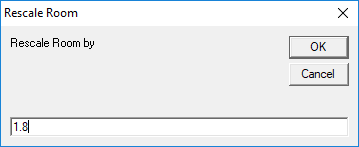
\includegraphics[width=0.5\textwidth]{archivos/capturas/ventanaescala.png}
    \caption{Ventana para modificar la escala del recinto en EASE.}
\end{figure}


Una vez escalado el recinto se simulará para obtener las curvas de los campos útil y perjudicial y ajustar a éstos las curvas de la teoría revisada corregida (sección \ref{teoriarevisadacorregida}) para obtener los coeficientes de ajuste (apartado \ref{metodocoeficientes}).

Los coeficientes obtenidos mediante el escalado y posterior ajuste se muestran en tablas relacionándolos con las dimensiones del recinto y el tiempo de reverberación en el capítulo de resultados y, en el anexo \ref{tablascompletas}, se encuentran todos los datos de cálculo.


\subsection{Método de obtención de coeficientes}
\label{metodocoeficientes}
En el programa EASEPostFile2Matlab (sección \ref{easepostfile2matlab}) se puede realizar todo el proceso de obtención de los coeficientes a partir de los datos obtenidos con EASE.

Los coeficientes se obtienen ajustando mediante regresión las ecuaciones de la teoría revisada corregida (sección \ref{teoriarevisadacorregida}) con las curvas de los campos acústicos obtenidos con EASE, en concreto se obtienen los 3 campos acústicos (directo, primeras reflexiones y cola reverberante). A continuación se muestran los códigos que realizan la regresión:

\begin{description}
\itemsep0em
  \item[Campo directo:]~
\vspace{-0.3cm}
\end{description}
\begin{lstlisting}[style=Matlab-color,numbers=none, caption={Líneas de código Matlab para obtener coeficientes de la teoría revisada corregida del campo directo.},label=coefdirect]
% Parámetros de la regresión
fD = fittype('Fac * W*Q./(4*pi*dist.^2)*Cd',... % Ecuación de campo directo
                'dependent',{'y'},...			% Curva de campo directo EASE
                'independent',{'dist'},...		% Vector de distancia
                'problem', {'Q','W','Fac'},...	% Constantes
                'coefficients',{'Cd'});			% Coeficiente
% Regresión
[fitiD,gofD,outputD] = fit(Distplot',10.^(Dplot'/10),fD,'problem',{Q,W,Fac})
\end{lstlisting}

\begin{description}
\itemsep0em
  \item[Campo tardío o cola reverberante:]~
  \vspace{-0.3cm}
\end{description}
\begin{lstlisting}[style=Matlab-color,numbers=none, caption={Líneas de código Matlab para obtener coeficientes de la teoría revisada corregida del campo tardío.},label=coefreverb]
% Parámetros de la regresión
fL = fittype('Fac * (4*W)/(S*(-log(1-alpha))) * exp(-(13.82*(dist/c+t)*el/T)) * Cl',... % Ecu. campo tardío
                'dependent',{'y'},... % Curva de campo tardío EASE
                'independent',{'dist'},... % Vector de distancia
                'problem', {'W','S','alpha','t','T','c','Fac'},... % Constantes
                'coefficients',{'el','Cl'}); % Coeficientes
% Regresión
[fitiL,gofL,outputL] = fit(Distplot',10.^(Pplot'/10),fL,'problem',{W,S,alpha,t,T,c,Fac});
\end{lstlisting}

\begin{description}
\itemsep0em
  \item[Primeras reflexiones:]~
  \vspace{-0.3cm}
\end{description}
\begin{lstlisting}[style=Matlab-color,numbers=none, caption={Líneas de código Matlab para obtener coeficientes de la teoría revisada corregida del campo temprano.},label=coeftemprano]
% Parámetros de la regresión
fE = fittype('Fac * ((4*W)./(S*(-log(1-alpha))*dist) .* (exp(-(13.82*(dist/c)*ee/T))*Ce - exp(-(13.82*(dist/c+t)*el/T)) * Cl))',... % Ecuación de primeras reflexiones
                'dependent',{'y'},... % Curva de primeras reflexiones EASE
                'independent',{'dist'},... % Vector de distancia
                'problem', {'W','S','alpha','T','t','c','Fac','el','Cl'},... % Constantes
                'coefficients',{'ee','Ce'}); % Coeficientes
% Regresión
[fitiE,gofE,outputE] = fit(Distplot',10.^(Eplot'/10),fE,'problem',{W,S,alpha,T,t,c,Fac,fitiL.el,fitiL.Cl});
\end{lstlisting}


Las variables vistas en los códigos anteriores corresponden a los siguientes parámetros:
\begin{itemize}
\itemsep0em
  \item \textbf{\textit{Distplot, Dist}}: Vector de distancia desde la distancia del receptor más cercano hasta el más lejano en incrementos de 0.01 metros.
  \item \textbf{\textit{Dplot, Pplot, Eplot}}: Son las curvas de los campos directo, tardío y temprano en decibelios obtenido con EASE.
  \item \textbf{\textit{y}}: Es el campo en lineal al que debe ajustarse la ecuación.
  \item \textbf{\textit{Fac}}: es el factor $Z/p_0^2$ que multiplica a la ecuación de la curva para obtenerla directamente en valores de presión acústica.
  \item \textbf{\textit{W, Q}}: Son la potencia y directividad de la fuente.
  \item \textbf{\textit{t}}: Es el periodo de integración temporal, 0.05 s.
  \item \textbf{\textit{alpha, T, c, S}}: El resto de parámetros que corresponden respectivamente a: coeficiente medio de absorción, tiempo de reverberación de Eyring, velocidad del sonido y superficie del recinto.
\end{itemize}


Los coeficientes y ecuaciones se encuentran en las variables \textit{fitiD}, \textit{fitiL} y \textit{fitiE} y la información de la regresión (valor de ajuste, etc) en \textit{gofD}, \textit{gofL} y \textit{gofE}.




\begin{figure}[ht]
    \centering%
    {\scalefont{0.8}%
    %%%%%%%%%%%%%%%%%%%%%%%%%%%%%%%%%%%%%%%%%%%%%%%%%%%%%%%%%%%%%%%%%%%%%%%%
% Escuela Politécnica Superior de la Universidad de Alicante
% Realizado por: Jose Manuel Requena Plens
% Contacto: info@jmrplens.com / Telegram:@jmrplens
%%%%%%%%%%%%%%%%%%%%%%%%%%%%%%%%%%%%%%%%%%%%%%%%%%%%%%%%%%%%%%%%%%%%%%%%

\definecolor{mycolor1}{rgb}{0.00000,0.00000,0.83333}%
\definecolor{mycolor2}{rgb}{0.00000,0.66667,1.00000}%
\definecolor{mycolor3}{rgb}{1.00000,0.83333,0.00000}%
\definecolor{mycolor4}{rgb}{0.00000,0.83333,1.00000}%
%
\begin{tikzpicture}

\begin{axis}[%
width=0.8\textwidth,
height=0.3\textwidth,
at={(0\textwidth,0\textwidth)},
scale only axis,
xmin=0,
xmax=20,
xlabel style={font=\color{white!15!black}},
xlabel={Distancia (m)},
ymin=55,
ymax=90,
minor x tick num= 1,
minor y tick num= 4,
ylabel style={font=\color{white!15!black}},
ylabel={SPL (dB)},
axis background/.style={fill=white},
xmajorgrids,
xminorgrids,
ymajorgrids,
%yminorgrids,
clip=false,
pin distance=0.1cm,
legend style={legend cell align=left, align=left, draw=white!15!black}
]


% DIRECTO
% errores
\addplot [color=mycolor1, draw=none]
 plot [error bars/.cd, y dir = both, y explicit]
 table[row sep=crcr, y error plus index=2, y error minus index=3]{%
1.17046999107196	81.0766819329314	2.11273863194452	2.11985110008034\\
2.78747197295327	74.5739935356949	2.63596035293671	2.68665772839481\\
4.04598566482878	71.9444086888792	2.82798882824397	2.89924555594612\\
4.77179211617606	70.80974979944	2.90722719572553	2.98786646759177\\
5.44357419348722	69.916830267974	2.96801913583234	3.05625623426916\\
6.68075594525051	68.5507871852776	3.05831719585986	3.15853967621463\\
7.02637886823647	68.2184523889925	3.07978487597832	3.18298885910806\\
7.46793144049944	67.8190441967531	3.10532387079679	3.21214487763349\\
7.66615940350838	67.6480791160366	3.11616817903356	3.22454867595874\\
8.58894638474359	66.911314351426	3.16229721149389	3.2774749798852\\
8.81093071133805	66.7470150098814	3.17244971819232	3.28916020866626\\
10.1498768465435	65.8434164779264	3.22740305679189	3.35265266585594\\
10.3329569823938	65.7301056372425	3.23418824452122	3.3605216845382\\
10.863701026814	65.4136625187782	3.25301145929897	3.38238701256432\\
12.2890194889584	64.6412993473262	3.29817249303285	3.43506728401826\\
12.6400158227749	64.4661465209575	3.30825868273846	3.44687713587695\\
13.2200605142337	64.1880675417193	3.32415334957864	3.46552231709151\\
14.4142290810157	63.65546351546	3.35418844660956	3.50087310726452\\
15.1334067545943	63.3575522053486	3.37075358380153	3.52043873365221\\
15.621139523095	63.1642155260982	3.3814133066721	3.5330560741706\\
16.6439178080162	62.7794378731708	3.40241512035242	3.55797813524529\\
17.1295067062657	62.6057338814364	3.41180290958454	3.56914619931278\\
17.5618905588208	62.4555466038525	3.41987282009681	3.57876062031445\\
18.4775539506721	62.1504554246786	3.43613168934562	3.59817197716738\\
};

% ease
\addplot [color=mycolor1, line width=1.2pt]
  table[row sep=crcr]{%
1.17046999107197	81.0766819329314\\
1.27046999107196	80.4388029844697\\
1.37046999107196	79.8537423556621\\
1.48046999107196	79.2619469593335\\
1.59046999107196	78.7165111298351\\
1.71046999107196	78.1667800695578\\
1.83046999107196	77.6577965123033\\
1.95046999107197	77.1841493569784\\
2.08046999107196	76.7058091797141\\
2.21046999107196	76.2591719284107\\
2.35046999107196	75.8093005457148\\
2.49046999107196	75.3878929286526\\
2.64046999107197	74.9642821734217\\
2.79046999107196	74.5662703668623\\
2.95046999107197	74.1667892604279\\
3.11046999107197	73.790383449802\\
3.28046999107197	73.4130338411823\\
3.45046999107197	73.0565396558131\\
3.63046999107196	72.699479727962\\
3.81046999107197	72.3613222123538\\
4.00046999107197	72.0228717164573\\
4.19046999107196	71.7016032538885\\
4.39046999107197	71.3802387523964\\
4.60046999107196	71.0596381273903\\
4.81046999107197	70.7546954791999\\
5.03046999107197	70.4505027746453\\
5.25046999107197	70.1605579598028\\
5.48046999107197	69.871341326205\\
5.72046999107197	69.5834051394313\\
5.97046999107197	69.2972258682055\\
6.22046999107197	69.0238929413401\\
6.48046999107197	68.7521166816444\\
6.75046999107197	68.4822582278681\\
7.03046999107197	68.2146266568921\\
7.32046999107196	67.949484246977\\
7.62046999107196	67.687051411099\\
7.93046999107196	67.4275112739734\\
8.25046999107197	67.1710138824845\\
8.58046999107196	66.9176800512227\\
8.92046999107197	66.6676048534302\\
9.27046999107196	66.4208607735723\\
9.63046999107196	66.1775005415453\\
10.000469991072	65.9375596707182\\
10.390469991072	65.6949638252811\\
10.790469991072	65.456304322344\\
11.200469991072	65.2215399421573\\
11.630469991072	64.9852368241312\\
12.070469991072	64.753152737053\\
12.530469991072	64.5202333035599\\
13.010469991072	64.2869758595955\\
13.500469991072	64.0583946732088\\
14.010469991072	63.8299477470499\\
14.540469991072	63.6020061699709\\
15.090469991072	63.3748985342493\\
15.660469991072	63.1489142002229\\
16.250469991072	62.9243065135456\\
16.860469991072	62.7012959241857\\
17.490469991072	62.4800729705186\\
18.150469991072	62.2574953134327\\
18.470469991072	62.1527516130678\\
}node [pos=1,pin=90:Directo] {};


% ajuste
\addplot [color=black, dotted, line width=1.5pt]
  table[row sep=crcr]{%
1.17046999107197	81.7695238494663\\
1.27046999107196	81.0574412945112\\
1.38046999107196	80.336190115049\\
1.49046999107196	79.6702647924639\\
1.61046999107197	78.9976767862028\\
1.73046999107196	78.3734480733897\\
1.86046999107197	77.7442761340348\\
1.99046999107196	77.1576168327421\\
2.13046999107196	76.5672210953246\\
2.27046999107196	76.014414197418\\
2.42046999107197	75.458735468273\\
2.57046999107196	74.9364787597153\\
2.72046999107197	74.4438507278716\\
2.88046999107196	73.9474624194843\\
3.04046999107196	73.4779150939051\\
3.21046999107196	73.0053572244104\\
3.38046999107196	72.557187821162\\
3.56046999107197	72.106582926423\\
3.74046999107196	71.6782060240527\\
3.93046999107196	71.2478398248451\\
4.13046999107196	70.8167400960577\\
4.33046999107196	70.4060288528439\\
4.54046999107196	69.9947133274803\\
4.75046999107197	69.6019979414524\\
4.97046999107197	69.2087803987638\\
5.20046999107197	68.8158776279289\\
5.43046999107196	68.4399811587338\\
5.67046999107197	68.0643483923082\\
5.91046999107196	67.7042891879621\\
6.16046999107196	67.344452593512\\
6.42046999107197	66.9853931121202\\
6.69046999107196	66.6275969792475\\
6.96046999107196	66.2839582126187\\
7.24046999107196	65.9413943630978\\
7.53046999107197	65.6002878770712\\
7.83046999107196	65.2609729301821\\
8.13046999107196	64.9344164968995\\
8.44046999107196	64.6093969182658\\
8.76046999107196	64.286181395263\\
9.09046999107197	63.965002771327\\
9.43046999107196	63.6460627724498\\
9.78046999107197	63.3295350231828\\
10.140469991072	63.0155678376543\\
10.510469991072	62.7042867894943\\
10.890469991072	62.3957970680184\\
11.280469991072	62.0901856304298\\
11.680469991072	61.7875231613546\\
12.090469991072	61.4878658519344\\
12.520469991072	61.184316888114\\
12.960469991072	60.8843145044931\\
13.410469991072	60.5878495479622\\
13.880469991072	60.2886460904787\\
14.360469991072	59.9933564454829\\
14.850469991072	59.7019255505932\\
15.360469991072	59.4086394370601\\
15.880469991072	59.1194624918176\\
16.420469991072	58.829017851954\\
16.970469991072	58.5428521187516\\
17.540469991072	58.2559050017818\\
18.130469991072	57.9685482743288\\
18.470469991072	57.8071705922665\\
};


% EARLY
% errores
\addplot [color=teal, draw=none]
 plot [error bars/.cd, y dir = both, y explicit]
 table[row sep=crcr, y error plus index=2, y error minus index=3]{%
1.17046999107196	86.1396879918656	1.0482559847345	1.04987798141723\\
2.78747197295327	82.6375552630342	1.36453966863168	1.37656930685714\\
4.04598566482878	81.1778300624663	1.49134507324204	1.50854737520064\\
4.77179211617606	80.5396742381478	1.54583356784666	1.56545086662283\\
5.44357419348722	80.0338486675846	1.58860958022049	1.61020735012616\\
6.68075594525051	79.2536686889753	1.6538646523947	1.67863175398938\\
7.02637886823647	79.0626833346098	1.66970462035881	1.69526873186653\\
7.46793144049944	78.8325314638438	1.68872251490744	1.71525813239739\\
7.66615940350838	78.7338073172529	1.69685662958186	1.72381267565044\\
8.58894638474359	78.3069166605818	1.73186522794373	1.76066478096885\\
8.81093071133805	78.2113973050061	1.73966207063803	1.76887979592169\\
10.1498768465435	77.6839394224651	1.78247464185017	1.81403884986626\\
10.3329569823938	77.6175399088373	1.78783507299656	1.81969914687546\\
10.863701026814	77.4318001752063	1.80279521036564	1.83550341277356\\
12.2890194889584	76.976544353002	1.83924677787729	1.87405704617703\\
12.6400158227749	76.8729232234626	1.84750048843679	1.88279576668819\\
13.2200605142337	76.7081189276564	1.86059462376767	1.89666629074796\\
14.4142290810157	76.3914628347635	1.88563985133524	1.92322051045194\\
15.1334067545943	76.2137597266754	1.89962907439408	1.93806648124581\\
15.621139523095	76.0982098314515	1.90869999619159	1.94769831973767\\
16.6439178080162	75.8677118936711	1.92673456667025	1.96686079692051\\
17.1295067062657	75.7634228998131	1.93486800225996	1.97550848977376\\
17.5618905588208	75.6731354418356	1.94189620027278	1.98298388110361\\
18.4775539506721	75.4893878146064	1.95616148721611	1.9981649375829\\
};

% ease
\addplot [color=teal, line width=1.2pt]
  table[row sep=crcr]{%
1.17046999107197	86.1396879918656\\
1.27046999107196	85.8025601117808\\
1.38046999107196	85.4624364432016\\
1.49046999107196	85.1496002520364\\
1.61046999107197	84.8347964568083\\
1.73046999107196	84.5436685850982\\
1.86046999107197	84.2512462447231\\
1.99046999107196	83.9794939513587\\
2.13046999107196	83.7068957886407\\
2.27046999107196	83.452455386067\\
2.42046999107197	83.1974726110279\\
2.58046999107196	82.9431302994181\\
2.74046999107196	82.7048024072411\\
2.91046999107196	82.4670518088709\\
3.09046999107196	82.2306790525461\\
3.27046999107196	82.0083123504341\\
3.46046999107196	81.7870939191339\\
3.66046999107196	81.5675786237214\\
3.87046999107196	81.3502196536683\\
4.09046999107197	81.1353821314339\\
4.31046999107197	80.9323256061089\\
4.54046999107196	80.7313353556087\\
4.78046999107197	80.5326749342877\\
5.03046999107197	80.3365545375321\\
5.30046999107196	80.1358996763959\\
5.58046999107196	79.9388223668422\\
5.87046999107196	79.7453415322106\\
6.17046999107197	79.5554546020688\\
6.49046999107196	79.3632879515291\\
6.82046999107196	79.1752457056077\\
7.17046999107197	78.9859511654149\\
7.53046999107197	78.8010915904308\\
7.91046999107196	78.6157490403454\\
8.31046999107197	78.4304701704895\\
8.72046999107197	78.2500145330986\\
9.15046999107196	78.0700669347323\\
9.60046999107196	77.8909999768856\\
10.070469991072	77.7131298886392\\
10.570469991072	77.5332124476798\\
11.090469991072	77.3553209659547\\
11.630469991072	77.1796086069738\\
12.200469991072	77.003176020993\\
12.800469991072	76.8265539468373\\
13.430469991072	76.650202419599\\
14.090469991072	76.474517029211\\
14.780469991072	76.299835205159\\
15.500469991072	76.1264423305375\\
16.260469991072	75.9523425667231\\
17.050469991072	75.7801847554573\\
17.880469991072	75.6080897735957\\
18.470469991072	75.4907724369276\\
}node [pos=0.15,pin=18:Temprano] {};

% ajuste
\addplot [color=black, dotted, line width=1.5pt]
  table[row sep=crcr]{%
1.17046999107197	86.2624183404492\\
1.27046999107196	85.91604716467\\
1.38046999107196	85.5660244420076\\
1.49046999107196	85.2436290612545\\
1.61046999107197	84.9188227608267\\
1.73046999107196	84.6181544861834\\
1.86046999107197	84.3159219048477\\
1.99046999107196	84.0348977063794\\
2.13046999107196	83.752898787596\\
2.27046999107196	83.489639807478\\
2.42046999107197	83.2258239886445\\
2.57046999107196	82.9786579761324\\
2.73046999107196	82.7312357468153\\
2.90046999107196	82.4846046350462\\
3.07046999107196	82.252842536919\\
3.25046999107197	82.0218683730331\\
3.44046999107196	81.7924144795613\\
3.63046999107196	81.5761348662079\\
3.83046999107196	81.3612206220439\\
4.04046999107196	81.1481936458785\\
4.26046999107196	80.9374882906805\\
4.49046999107196	80.7294620052275\\
4.73046999107196	80.5244051674098\\
4.98046999107196	80.3225500260486\\
5.24046999107196	80.1240787303107\\
5.51046999107196	79.929130467809\\
5.79046999107196	79.7378077591634\\
6.08046999107196	79.550181972232\\
6.38046999107196	79.3662981266579\\
6.69046999107196	79.1861790613249\\
7.02046999107196	79.0044651029292\\
7.36046999107197	78.8270602803765\\
7.72046999107197	78.6490730398285\\
8.09046999107197	78.4757326423053\\
8.48046999107197	78.3025811258486\\
8.89046999107197	78.13015915289\\
9.31046999107197	77.9628124640686\\
9.75046999107197	77.7966563750721\\
10.210469991072	77.6320651246229\\
10.690469991072	77.469358627971\\
11.200469991072	77.3056842368369\\
11.730469991072	77.1447254045417\\
12.280469991072	76.9866434427519\\
12.860469991072	76.8289211980065\\
13.470469991072	76.672087819123\\
14.100469991072	76.5189661338561\\
14.760469991072	76.3673296895826\\
15.460469991072	76.2154288999106\\
16.190469991072	76.0659167719822\\
16.950469991072	75.9190359265717\\
17.750469991072	75.7732179520838\\
18.470469991072	75.6490240539378\\
};


% LATE
% errores
\addplot [color=red, draw=none]
 plot [error bars/.cd, y dir = both, y explicit]
 table[row sep=crcr, y error plus index=2, y error minus index=3]{%
1.17046999107196	79.7499907626293	0.250293597968906	0.25029359796892\\
2.78747197295327	79.4463211373774	0.282335503570266	0.28233550357028\\
4.04598566482878	79.209974870973	0.30727373949388	0.30727373949388\\
4.77179211617606	79.0736699217178	0.321656048272416	0.321656048272416\\
5.44357419348722	78.9475106380843	0.33496783029068	0.334967830290665\\
6.68075594525051	78.7151704658791	0.359483360479203	0.359483360479203\\
7.02637886823647	78.6502631963287	0.366332094862997	0.366332094863012\\
7.46793144049944	78.5673405372036	0.375081735245033	0.375081735245033\\
7.66615940350838	78.5301137360519	0.379009746310857	0.379009746310842\\
8.58894638474359	78.3568162510031	0.397295347487727	0.397295347487727\\
8.81093071133805	78.3151280539421	0.401694105756064	0.401694105756079\\
10.1498768465435	78.0636767411631	0.428226160849562	0.428226160849562\\
10.3329569823938	78.0292946705981	0.431854008246248	0.431854008246233\\
10.863701026814	77.9296220376146	0.442371033432565	0.442371033432579\\
12.2890194889584	77.6619501806139	0.470614610204677	0.470614610204677\\
12.6400158227749	77.5960337956316	0.477569822084803	0.477569822084803\\
13.2200605142337	77.4871026031789	0.489063770426583	0.489063770426583\\
14.4142290810157	77.2628402180826	0.512726967452735	0.512726967452735\\
15.1334067545943	77.1277801395717	0.526977922853916	0.526977922853916\\
15.621139523095	77.0361849351791	0.53664265270713	0.53664265270713\\
16.6439178080162	76.8441092902646	0.55690964410465	0.556909644104664\\
17.1295067062657	76.7529167002677	0.566531891827978	0.566531891827992\\
17.5618905588208	76.671715907726	0.575099848294556	0.57509984829457\\
18.4775539506721	76.4997562180187	0.593244291092446	0.593244291092446\\
};

% ease
\addplot [color=red, line width=1.2pt]
  table[row sep=crcr]{%
1.17046999107197	79.7499907626293\\
18.470469991072	76.5010865709689\\
}node [pos=0.9,pin=90:Reverberante] {};


% ajuste
\addplot [color=black, dotted, line width=1.5pt]
  table[row sep=crcr]{%
1.17046999107197	79.7499907626293\\
18.470469991072	76.5010865709689\\
};


\end{axis}
\end{tikzpicture}%%
    }
    \caption{Ejemplo de ajuste de los tres campos acústicos por separado para el aula OP/S003 simulada en EASE y ajustada mediante regresión (líneas discontinuas).}%
    \label{graf:trescamposajuste}%
\end{figure}
\FloatBarrier


\section{Inteligibilidad}
\label{desarrollointeligibilidad}
Una vez se obtienen las ecuaciones ajustadas para determinar los campos acústicos a cualquier distancia, es posible utilizarlas para calcular parámetros que habitualmente se obtienen mediante medidas o simulaciones pesadas.

Teniendo en cuenta las definiciones de claridad (apartado \ref{claridad}), definición (apartado \ref{definicion}) y sonoridad (apartado \ref{sonoridad}) es posible obtener estos parámetros a través de las curvas de los campos tal que:

\begin{flalign}
	C_{50} =& L_{p,\text{útil}} - L_{p,\text{perjudicial}}
\end{flalign}
\begin{flalign}
	D_{50} =& \frac{ 10^{\nicefrac{L_{p,\text{útil}}}{10}} }{ 10^{\nicefrac{L_{p,\text{útil}}}{10}}+10^{\nicefrac{L_{p,\text{perjudicial}}}{10}} }
\end{flalign}
\begin{flalign}
	G =& 10\log_{10}\left(\frac{10^{\nicefrac{L_{p,\text{útil}}}{10}}+10^{\nicefrac{L_{p,\text{perjudicial}}}{10}}}{\left(\nicefrac{Z}{p_0^2}\right)I_{D,\text{10m}}}\right)
\end{flalign}
\begin{condiciones}[Donde:]
	\nicefrac{Z}{p_0^2} & \rightarrow & Es el factor necesario para obtener valores de presión normalizados por medio de valores de intensidad.\\
	I_{D,\text{10m}} & \rightarrow & Es la intensidad del campo directo corregido a 10 metros.
\end{condiciones}


En este caso se obtiene para todo el espectro de frecuencias y no para las recomendadas para claridad y definición, pero se puede tomar en consideración y equiparar. Esta solución permite calcular de forma teórica los parámetros de claridad, definición y sonoridad a través de la teoría revisada corregida.

En el caso de parámetros que necesiten ser procesados en bandas de frecuencia, como el índice de articulación (apartado \ref{indicearticulacion}), no es posible calcularlo, para ello sería preciso encontrar una relación entre las respuesta en frecuencia de la fuente y la teoría revisada corregida para obtener niveles por bandas de frecuencia. Por el momento no se ha profundizado en esta cuestión aunque en futuros estudios se planteará.
